% Options for packages loaded elsewhere
\PassOptionsToPackage{unicode}{hyperref}
\PassOptionsToPackage{hyphens}{url}
%
\documentclass[
]{article}
\usepackage{lmodern}
\usepackage{amssymb,amsmath}
\usepackage{ifxetex,ifluatex}
\ifnum 0\ifxetex 1\fi\ifluatex 1\fi=0 % if pdftex
  \usepackage[T1]{fontenc}
  \usepackage[utf8]{inputenc}
  \usepackage{textcomp} % provide euro and other symbols
\else % if luatex or xetex
  \usepackage{unicode-math}
  \defaultfontfeatures{Scale=MatchLowercase}
  \defaultfontfeatures[\rmfamily]{Ligatures=TeX,Scale=1}
\fi
% Use upquote if available, for straight quotes in verbatim environments
\IfFileExists{upquote.sty}{\usepackage{upquote}}{}
\IfFileExists{microtype.sty}{% use microtype if available
  \usepackage[]{microtype}
  \UseMicrotypeSet[protrusion]{basicmath} % disable protrusion for tt fonts
}{}
\makeatletter
\@ifundefined{KOMAClassName}{% if non-KOMA class
  \IfFileExists{parskip.sty}{%
    \usepackage{parskip}
  }{% else
    \setlength{\parindent}{0pt}
    \setlength{\parskip}{6pt plus 2pt minus 1pt}}
}{% if KOMA class
  \KOMAoptions{parskip=half}}
\makeatother
\usepackage{xcolor}
\IfFileExists{xurl.sty}{\usepackage{xurl}}{} % add URL line breaks if available
\IfFileExists{bookmark.sty}{\usepackage{bookmark}}{\usepackage{hyperref}}
\hypersetup{
  pdftitle={Análisis de expresión diferencial de RNA-seq de muestras de tiroides con distintos tipos de infiltración},
  pdfauthor={Marc Expòsit Goy},
  hidelinks,
  pdfcreator={LaTeX via pandoc}}
\urlstyle{same} % disable monospaced font for URLs
\usepackage[margin=1in]{geometry}
\usepackage{color}
\usepackage{fancyvrb}
\newcommand{\VerbBar}{|}
\newcommand{\VERB}{\Verb[commandchars=\\\{\}]}
\DefineVerbatimEnvironment{Highlighting}{Verbatim}{commandchars=\\\{\}}
% Add ',fontsize=\small' for more characters per line
\usepackage{framed}
\definecolor{shadecolor}{RGB}{248,248,248}
\newenvironment{Shaded}{\begin{snugshade}}{\end{snugshade}}
\newcommand{\AlertTok}[1]{\textcolor[rgb]{0.94,0.16,0.16}{#1}}
\newcommand{\AnnotationTok}[1]{\textcolor[rgb]{0.56,0.35,0.01}{\textbf{\textit{#1}}}}
\newcommand{\AttributeTok}[1]{\textcolor[rgb]{0.77,0.63,0.00}{#1}}
\newcommand{\BaseNTok}[1]{\textcolor[rgb]{0.00,0.00,0.81}{#1}}
\newcommand{\BuiltInTok}[1]{#1}
\newcommand{\CharTok}[1]{\textcolor[rgb]{0.31,0.60,0.02}{#1}}
\newcommand{\CommentTok}[1]{\textcolor[rgb]{0.56,0.35,0.01}{\textit{#1}}}
\newcommand{\CommentVarTok}[1]{\textcolor[rgb]{0.56,0.35,0.01}{\textbf{\textit{#1}}}}
\newcommand{\ConstantTok}[1]{\textcolor[rgb]{0.00,0.00,0.00}{#1}}
\newcommand{\ControlFlowTok}[1]{\textcolor[rgb]{0.13,0.29,0.53}{\textbf{#1}}}
\newcommand{\DataTypeTok}[1]{\textcolor[rgb]{0.13,0.29,0.53}{#1}}
\newcommand{\DecValTok}[1]{\textcolor[rgb]{0.00,0.00,0.81}{#1}}
\newcommand{\DocumentationTok}[1]{\textcolor[rgb]{0.56,0.35,0.01}{\textbf{\textit{#1}}}}
\newcommand{\ErrorTok}[1]{\textcolor[rgb]{0.64,0.00,0.00}{\textbf{#1}}}
\newcommand{\ExtensionTok}[1]{#1}
\newcommand{\FloatTok}[1]{\textcolor[rgb]{0.00,0.00,0.81}{#1}}
\newcommand{\FunctionTok}[1]{\textcolor[rgb]{0.00,0.00,0.00}{#1}}
\newcommand{\ImportTok}[1]{#1}
\newcommand{\InformationTok}[1]{\textcolor[rgb]{0.56,0.35,0.01}{\textbf{\textit{#1}}}}
\newcommand{\KeywordTok}[1]{\textcolor[rgb]{0.13,0.29,0.53}{\textbf{#1}}}
\newcommand{\NormalTok}[1]{#1}
\newcommand{\OperatorTok}[1]{\textcolor[rgb]{0.81,0.36,0.00}{\textbf{#1}}}
\newcommand{\OtherTok}[1]{\textcolor[rgb]{0.56,0.35,0.01}{#1}}
\newcommand{\PreprocessorTok}[1]{\textcolor[rgb]{0.56,0.35,0.01}{\textit{#1}}}
\newcommand{\RegionMarkerTok}[1]{#1}
\newcommand{\SpecialCharTok}[1]{\textcolor[rgb]{0.00,0.00,0.00}{#1}}
\newcommand{\SpecialStringTok}[1]{\textcolor[rgb]{0.31,0.60,0.02}{#1}}
\newcommand{\StringTok}[1]{\textcolor[rgb]{0.31,0.60,0.02}{#1}}
\newcommand{\VariableTok}[1]{\textcolor[rgb]{0.00,0.00,0.00}{#1}}
\newcommand{\VerbatimStringTok}[1]{\textcolor[rgb]{0.31,0.60,0.02}{#1}}
\newcommand{\WarningTok}[1]{\textcolor[rgb]{0.56,0.35,0.01}{\textbf{\textit{#1}}}}
\usepackage{graphicx,grffile}
\makeatletter
\def\maxwidth{\ifdim\Gin@nat@width>\linewidth\linewidth\else\Gin@nat@width\fi}
\def\maxheight{\ifdim\Gin@nat@height>\textheight\textheight\else\Gin@nat@height\fi}
\makeatother
% Scale images if necessary, so that they will not overflow the page
% margins by default, and it is still possible to overwrite the defaults
% using explicit options in \includegraphics[width, height, ...]{}
\setkeys{Gin}{width=\maxwidth,height=\maxheight,keepaspectratio}
% Set default figure placement to htbp
\makeatletter
\def\fps@figure{htbp}
\makeatother
\setlength{\emergencystretch}{3em} % prevent overfull lines
\providecommand{\tightlist}{%
  \setlength{\itemsep}{0pt}\setlength{\parskip}{0pt}}
\setcounter{secnumdepth}{-\maxdimen} % remove section numbering
\usepackage{flafter}
\usepackage{booktabs}
\usepackage{longtable}
\usepackage{array}
\usepackage{multirow}
\usepackage{wrapfig}
\usepackage{float}
\usepackage{colortbl}
\usepackage{pdflscape}
\usepackage{tabu}
\usepackage{threeparttable}
\usepackage{threeparttablex}
\usepackage[normalem]{ulem}
\usepackage{makecell}
\usepackage{xcolor}

\title{Análisis de expresión diferencial de \emph{RNA-seq} de muestras de
tiroides con distintos tipos de infiltración}
\author{Marc Expòsit Goy}
\date{Junio 2020}

\begin{document}
\maketitle

{
\setcounter{tocdepth}{3}
\tableofcontents
}
\newpage

\hypertarget{abstract}{%
\section{1. Abstract}\label{abstract}}

En este estudio se identifican las redes biológicas afectadas por el
tamaño de infiltración cancerígena en muestras de tiroides de pacientes
humanos. Los datos se obtienen de la base de datos GTEx y corresponden a
análisis de RNA-Seq. Tras el análisis de expresión diferencial
utilizando \texttt{DESeq} en \texttt{R} y la anotación de los
tránscripts de interés, se identifican varios términos GO y rutas
biológicas KEGG que podrían informar de los cambios biológicos según el
tipo de infiltración del tejido.

\textbf{Los datos y scripts utilizados para el análisis pueden
encontrarse en un repositorio \texttt{GitHub}, acesible aquí:
\url{https://github.com/marcexpositg/exposit_marc_ADO_PEC2_MBio}}

\hypertarget{objetivos}{%
\section{2. Objetivos}\label{objetivos}}

\textbf{El estudio:} el objetivo del estudio es estudiar cambios en la
expresión génica de tejido de tiroides humano según el tamaño de
infiltraciones cancerígenas. Para ello, se parte de 10 muestras de cada
uno de los 3 tamaños distintos de infiltraciones (sin infiltración, NIT;
focal, SFI; o extensa, ELI), selecionadas aleatoriamente de un conjunto
de 292 muestras.

\textbf{La pregunta a responder:} identificar los procesos biológicos
afectados según el tamaño de infiltraciones cancerígenas en tejido
humano de tiroides, a partir de la comparación del nivel de expresión de
los genes.

\textbf{El método:} la expresión génica de cada muestra se analiza por
RNA-Seq para poder realizar un análisis de expresión diferencial
utilizando \texttt{R}. La identificación de genes con cambio de
expresión se realiza a partir de tres comparaciones a pares distintas
entre los 3 niveles de tamaño de infilitración.

\hypertarget{materiales-y-muxe9todos}{%
\section{3. Materiales y métodos}\label{materiales-y-muxe9todos}}

\hypertarget{descripciuxf3n-de-los-datos}{%
\subsection{3.1. Descripción de los
datos}\label{descripciuxf3n-de-los-datos}}

Los datos utilizados para el estudio se obtienen a partir del
repositorio del proyecto \emph{Gentoype-Tissue Expression}
(GTEx)(Lonsdale et al. 2013), que contiene datos de RNA-Seq y
\emph{Whole Genome Sequencing} de distintos tipos de tejido de casi 1000
individuos humanos. En este caso, se parte de 292 muestras con datos de
expresión de \textbf{RNA-Seq} para 56202 tránscritos. Estos pertenecen a
tejido de \textbf{tiroides} humana y las muestras se clasifican según el
tamaño de infiltración cancerígena del tejido:

\begin{itemize}
\tightlist
\item
  Sin infiltración (\emph{Not infiltrated tissues}, NIT): 236 muestras
\item
  Infiltraciones pequeñas y focales (\emph{Small focal infiltrates},
  SFI): 42 muestras
\item
  Infiltraciones limfóides extensas (\emph{Extensive lymphoid
  infiltrates}, ELI): 14 muestras
\end{itemize}

Para realizar el análisis de expresión diferencial, se selecionan
aleatoriamente 10 muestras de cada tipo de infiltración para teber el
mismo número de muestras de cada tipo. El efecto biológico a estudiar se
asesora a partir de \textbf{tres comparaciones a pares}: SFI-NIT,
ELI-NIT, y ELI-SFI. Ya que el tamaño de infiltración ordena las tres
categorías (NIT\textless SFI\textless ELI), a través de estas
comparaciones se comparan los dos niveles de infiltración (pequeña, SFI;
o grande, ELI) con tejido sin infiltrar (NIT), y los dos niveles de
infiltración entre ellos (SFI-ELI). De este modo se puede caracterizar
la muestra correctamente.

Por lo tanto, el diseño experimental corresponde a un solo factor
(tamaño de la infiltración) estudiado a tres niveles distintos
utilizando 10 réplicas para cada nivel. Así pues, el total de muestras
utilizado es de 30.

\hypertarget{pipeline-de-anuxe1lisis}{%
\subsection{3.2. Pipeline de análisis}\label{pipeline-de-anuxe1lisis}}

Brevemente, el estudio parte de una matriz de contajes que indica, para
cada una de las 292 muestras disponibles, el número de \emph{reads} o
contajes que se ha realizado para cada uno de los 56202 tránscrits
analizados por RNA-Seq. Por lo tanto, no se empieza a partir de la
\emph{raw data} (que serían los ficheros \texttt{FASTQ}) y se supone que
los datos en bruto han sido analizados para filtrar por calidad (quizás
con \texttt{FastQC}) y mapeados a los tránscritos para obtener la matriz
de contajes inicial (quizás con \texttt{tximport} y \texttt{Salmon}).
Junto con la matriz de datos, se proporciona información de las muestras
para categorizarlas según el tipo de infiltración. Después de selecionar
10 muestras aleatoriamente de cada clase, se filtran los datos iniciales
reduciendo el número de genes a comparar para disminuir el error de tipo
1 de los contrastes.

Con los datos iniciales preparados, se ha realizado un análisis
exporatorio inicial de los datos. Para ello, se crean gráficos de la
distribución de contajes de cada muestra, matrices de similitud entre
las muestras, y se realiza el análisis de componentes principales (PCA)
para identificar el orígen de la varianza entre las muestras.

El análisis de expresión diferencial se realiza para las tres
comparaciones utilizando las funciones de la liberería \texttt{DeSeq2}
dentro de \texttt{Bioconductor} en \texttt{R}. Para la interpretación de
los resultados, se han anotado los tránscritos con las IDs de Entrez y
el nombre del gen al que pertenecen, utilizando la librería
\texttt{org.Hs.eg.db} de \texttt{AnnotationDbi}. Con los tránscripts
anotados, se crean tablas para mostrar los genes que se encuentran más
diferencialmente expresados en cada una de las tres comparaciones.
También se utilizan gráficos como los gráficos MA o \emph{Volcano Plots}
para mostrar la distribución de los tránscritos según las condiciones.

Para entender bien la cuestión del estudio, se han comparado los 3
contrastes entre ellos. Esto permite identificar aquellos genes cuya
expresión cambia en todas las muestras, solamente en una o en dos de
ellas, y crear grupos de interés para estudiar con más detalle. Para
esto, se han utilizado diagramas de Venn y \emph{heatmaps}.

Finalmente, a partir de los genes que se hallan diferencialmente
expresados en uno de los grupos anteriores, se ha utilizado
\texttt{clustrProfilr} para anotar los términos GO que se encuentran
diferencialmente expresados y las vías metabolicas en las que están
implicados, junto con una visualización de como cambia una de estas
redes. El análisis de \emph{Gene Enrichment} permite dotar de sentido
biológico al análisis realizado con RNA-Seq y entender las diferencias
entre los grupos para resolver las questiones planteadas.

\hypertarget{preparaciuxf3n-de-los-datos}{%
\subsection{3.3. Preparación de los
datos}\label{preparaciuxf3n-de-los-datos}}

\hypertarget{importaciuxf3n-de-datos}{%
\subsubsection{3.3.1. Importación de
datos}\label{importaciuxf3n-de-datos}}

Los datos iniciales constan de una matriz de contajes (\emph{counts}) y
una matriz de información de las muestras en formato \texttt{csv}. Para
selecionar 10 muestras de cada clase, se descarta selecionar
aleatoriamente las columnas y filas de estas matrices por separado y
luego juntarlas en un objeto \texttt{SummarizedExperiment}, ya que hay
mayor riesgo de equivocación que en la aproximación descrita a
continuación. Por esto, se construye primero el objeto
\texttt{SummarizedExperiment}(Morgan et al. 2017) a partir de las dos
matrices. Este objeto es estándard y puede ser utilizado por varias
librerías y por varios tipos de datos, y guarda información que
relaciona cada muestra con su información y los counts de los genes. De
este modo, se puede obtener un \texttt{subset} a partir de este objeto
sin riesgo a cruzar muestras involuntariamente.

La seleción de 10 muestras de cada clase se realiza aleatoriamente
utilizando la semilla 456, y utilizando la función \texttt{sample} para
elegir entre los índices de cada categoría. Estos índices se utilizan
para seleccionar 10 muestras de cada grupo del objeto
\texttt{SummarizedExperiment} y mantenerlas en un mismo objeto.

Una vez el conjunto de datos a analizar está definido se crea un objeto
\texttt{DESeqDataSet} a partir del \texttt{SummarizedExperiment}. Nótese
que en este paso se \textbf{reordenan los factores} de \texttt{Group}
que indica el tipo de infiltración, de modo que \texttt{NIT} sea el
grupo basal con el que realizar las comparaciones, \texttt{SFI} el nivel
medio y \texttt{ELI} el nivel alto. También se especifica \textbf{el
diseño del experimento} que tendrá en cuenta solamente una variable, que
es el tipo de infiltración (\texttt{Group}). Con \texttt{DESeq2} no es
necesario crear una matriz experimental como pasa con \texttt{limma},
solamente debe especificarse
\texttt{design\ =\ \textasciitilde{}\ Group} en este caso y asegurarse
que el orden de los factores es correcto.

\hypertarget{filtraje-inicial}{%
\subsubsection{3.3.2. Filtraje inicial}\label{filtraje-inicial}}

Previamente a realizar los contrastes para identificar los genes
expresados diferencialmente, se filtran los datos. El proceso de
filtraje tiene por objetivo reducir el número de genes contrastados
estadísticamente, ya que el error de tipo I incrementa al realizar un
número elevado de comparaciones. Elegir el punto límite de filtraje es
delicado, ya que si se eliminaran demasiados genes podrían perderse
efectos importantes en el análisis. Por este motivo, se prueba de
aplicar distintos filtros para ver como cambia el número de muestras
estudiadas.

Un filtrado básico es eliminar aquellos genes cuyos tránscritos no se
han identificado o se han identificado una sola vez en las 30 muestras
comparadas (aquellos genes con \texttt{counts=0} o \texttt{counts=1}).
Estos genes no aportan información y eliminandolos se disminuye el
número de comparaciones realizadas, reduciendo el error de tipo I. Para
probar, también se crea un filtrado más \emph{agresivo}, que descartaría
aquellos genes que no lleguen a 5 counts en almenos 10 muestras de las
comparadas. Del total de 56202 tránscripts estudiados, el filtrado
básico elimina 9950 tránscripts con \texttt{count=0} y 2890 con
\texttt{count=1}. El filtrado más estricto eliminaría 25229 tránscripts
del conjunto (cerca del \(50\%\) de los datos).

En este caso, se toma \textbf{la decisión de mantener el filtro básico y
descartar aplicar un filtro que eliminaría el} \(50\%\) \textbf{de los
datos}. Seguramente, la información sobre el experimento y las preguntas
a responder permitiría saber si es preferible el error introducido al
comparar un elevado número de muestras o bien es preferible estudiar el
mayor número de genes posibles porqué es posible que haya interacciones.
Como no se dispone de esta información, se decide \textbf{escoger la
opción más conservativa} y con menos riesgo de perder información. Aún
así, el filtraje realizado ya avanza que un gran número de los genes
estudiados (cerca del \(50\%\)) tiene un número de \texttt{counts} bajo
(no llega ni a 5 counts en 10 de las muestras). Otro motivo por el que
se ha optado por un filtro suave es porqué al realizar el análisis de
expresión diferencial con \texttt{DESeq} esta función ya realiza un
filtrado simple. Tras el filtrado básico, el conjunto de datos pasa de
\textbf{56202 tránscripts a 43362}, conservando el \(77\%\) de los
datos.

\hypertarget{normalizaciuxf3n-y-anuxe1lisis-descriptivo}{%
\subsubsection{3.3.1. Normalización y análisis
descriptivo}\label{normalizaciuxf3n-y-anuxe1lisis-descriptivo}}

Para la exploración de datos multivariantes es importante asegurar la
homocedasticidad de los datos, es decir, que la varianza sea constante
independentmente de la media de las muestras. En el caso de los datos de
RNA-seq, la varianza incrementa con la media de cada muestra. Así, para
realizar análisis multivariantes con datos de RNA-Seq se ha aplicado un
proceso de normalización entre muestras que permita las comparaciones.

Esta normalización se fundamenta en tomar el logaritmo de base 2
(\texttt{log2}) de los \emph{counts} al que se añade un pseudo-contaje
de 1 para evitar el caso \(log_2(0)=-\infty\). Aún así, esto incrementa
el peso que tienen los datos con bajos valores de \emph{counts} en estos
análisis multivariantes. Estos datos son precisamente aquellos con menos
separación entre señal y ruido y por lo tanto, podrían introduir ruido
en el análisis. Para solucionarlo, el paquete \texttt{DESeq} introduce
dos posibles transformaciones: la \emph{variance stabilizing
transformation} (VST) y la\emph{regularized-logarithm transformation}
(rlog).

Las dos transformaciones son prácticamente idénticas al \texttt{log2}
para valores altos, pero difieren en como tratan los valores pequeños.
Para muestras de tamaño medio y grande (n\textgreater=30) es más
adecuado utilizar \texttt{VST}(Zhu, Ibrahim, and Love 2019) ya que es
más eficiente que \texttt{rlog}, además es menos sensible a outliers de
valores altos. \textbf{Como en este caso hay 30 muestras, se utiliza la
transformación VST}, implementada con la función \texttt{vst}.

Con los datos normalizados se visualiza la distribución de los
\texttt{counts} con un diagrama de cajas y un gráfico de densidad
utilizando las funciones gráficas base de \texttt{R}. Las distancias
entre las muestras se representan utilizando \texttt{pheatmap}, que crea
un mapa de intensidades de color (\emph{heatmap}) y ajunta las muestras
por clústers para su comparación. Finalmente, se analiza la variabilidad
de los datos con un \emph{Principal Component Analysis} (PCA) con
\texttt{plotPCA} y se presentan los resultados con \texttt{ggplot},
representando las muestras en sus primeras dos dimensiones de mayor
varianza e identificándolas según el tipo de infiltración y sexo del
individuo.

\hypertarget{identificaciuxf3n-de-genes-expresados-diferencialmente}{%
\subsection{3.4. Identificación de genes expresados
diferencialmente}\label{identificaciuxf3n-de-genes-expresados-diferencialmente}}

\hypertarget{anuxe1lisis-de-expresiuxf3n-diferencial}{%
\subsubsection{3.4.1. Análisis de expresión
diferencial}\label{anuxe1lisis-de-expresiuxf3n-diferencial}}

Para el análisis de expresión diferencial se escoje utilizar la librería
\texttt{DESeq2}(Love et al. 2015) en \texttt{R} por su versatibilidad,
abundancia de funciones que permiten analizar los resultados, y buena
calidad de documentación en la red. El análisis se realiza con los
\emph{counts} sin normalizar por VST, ya que \texttt{DESeq} tiene en
cuenta el tamaño de cada muestra para normalizar los datos antes del
análisis de forma automática. Además, no es necesario volver a
especificar la fórmula de diseño, puesto que ya se ha indicado al crear
el objeto \texttt{DESeqDataSet} con los datos para el análisis.

Durante el análisis también se calculan las distancias de Cook, con las
que se representan los datos para identificar posibles outliers.
Finalmente, se extraen los resultados con la función \texttt{results}
indicando los tres contrastes a realizar (según \texttt{Group}: SFI-NIT,
ELI-NIT, ELI-SFI). Las tablas resultantes contienen información como el
log2FoldChange, que indica el sentido (sobre- o infra- expresado) y
magnitud del efecto de cada tránscript en la comparación, y también el
\emph{p-valor} sin ajustar y ajustado por Benjamini-Hochberg (BH). En
adelante, solamente se utiliza el \emph{p-valor} ajustado por BH, puesto
que la correción reducie el error de tipo I introducido al hacer un
número tan alto de contrastes, reduciendo así la proporción de falsos
positivos.

En este estudio, se considera un gen como interesante de estudio o
significante aceptando un \emph{False Discovery Rate} (FDR) del
\(10\%\), así que se consideran significativos aquellos que tienen un
\emph{p-valor} ajustado por Benjamini-Hochberg \textbf{inferior a 0.1}.
En análisis de expresión diferencial también se suele aplicar un mínimo
de magnitud de efecto necesaria para considerar un gen significante (por
ejemplo, \texttt{log2FC\textgreater{}1} indicando que la expresión es el
doble en una muestra que en la otra). En este estudio, en cambio, se
estudian todos aquellos los genes cuyo \texttt{FoldChange} es diferente
a cero para no perder genes que quizás son importantes aunque su
magnitud de cambio sea pequeña.

\hypertarget{anotaciuxf3n-de-los-resultados}{%
\subsubsection{3.4.2. Anotación de los
resultados}\label{anotaciuxf3n-de-los-resultados}}

Para indentificar los tránscripts estudiados se parte del
\texttt{Ensembl\ gene\ ID} que se muestra para cada uno de los
tránscripts. Este se formatea para eliminar la versión indicada para
cada ID con un \texttt{.\#} detrás del ID. Para las anotaciones se
utiliza el paquete \texttt{org.Hs.eg.db} de anotaciones Ensembl de
Bioconductor. Para relacionar el código de cada transcript con el resto
de los datos se utiliza la función \texttt{mapIds}. La información
obtenida de cada tránscript es el nombre corto del gen
(\texttt{symbol}), su \texttt{EntrezID} y el nombre completo del gen al
que pertenece el transcript. Un total de 20860 tránscripts (cerca de la
mitad del total) no pueden ser relacionados por esta base de datos
porqué no todos aparecen en la base de datos. Con los tránscripts
anotados, se crean tablas para mostrar los 6 tránscritos más sobre- y
infra- regulados de cada grupo con mayor cambio de regulación (mayor
log2FoldChange) y significancia al \(10\%\). Gracias a la anotación, se
puede añadir para cada tránscrito información como el log2FoldChange
(efecto del gen), el p-valor ajustado (padj), el nombre abreviado del
gen al que pertenece y su entrez ID.

\hypertarget{visualizaciuxf3n}{%
\subsubsection{3.4.3. Visualización}\label{visualizaciuxf3n}}

Los resultados del análisis de expresión diferencial se visualizan con
gráficos MA utilizando las funciones \texttt{lfcShrink} y
\texttt{plotMA} de la librería \texttt{apeglm} para cada
comparación(Love, Anders, and Huber 2019). Para los genes de interés, se
puede visualizar el número de counts en cada muestra según el nivel
utilizando \texttt{plotCounts}. Además, los resultados del análisis de
expresión diferencial permiten agrupar los tránscritos según su valor en
cada muestra en función del grupo, para visualizar relaciones
interesantes. De forma similar a como se hizo para agrupar las muestras
según sus varianzas, se pueden agrupar las muestras y sus genes
expresados diferencialmente. Para ello, se seleccionan los 20 genes con
más expresión diferencial entre las muestras estudiadas y se representan
por grupos utilizando \texttt{pheatmap}(Phipson et al. 2016). Nótese que
se trabaja con los datos normalizados por VST. Finalmente, pueden
representarse los datos en un \emph{Volcano Plot}. En este se muestra su
\texttt{log2FoldChange} que indica el nivel del efecto y si es sobre- o
infra- expresión y su \emph{p-valor} ajustado que indica la
significancia de este cambio. Como ejemplo se representan los
tránscripts de la comparación ELI-NIT, indicando aquellos con cambio
significativo (p-valor ajustado\textless0.1) en color azul y añadiendo
el nombre de los 5 tránscripts con un menor p-valor.

\hypertarget{comparaciones-muxfaltiples}{%
\subsection{3.5. Comparaciones
múltiples}\label{comparaciones-muxfaltiples}}

Para identificar los grupos de genes que se encuentren diferencialmente
expresados en más de una comparación y obtener una imagen completa de
los datos se utiliza un diagrama de Venn. Para ello, se construye
\emph{manualmente} una matriz que indica si un gen es significativo al
\(10\%\) y sobre-expresado (+1) o infra-expresado (-1) o bien si no es
significativo y/o expresado diferencialmente (0), para cada comparación.
Esta matriz se adapta al formato de entrada que espera la función
\texttt{vennDiagram} del paquete \texttt{limma}, así que esta se utiliza
para representar el diagrama de Venn. Además, a partir de la matriz con
los datos del diagrama pueden selecionarse los tránscripts que
pertenezcan a una clase concreta (por ejemplo, sobre-expresados tanto en
SFI-NIT como en ELI-NIT), y utilizar la función \texttt{plotCounts} para
visualizar el número de \emph{counts} en cada muestra según el nivel.

\hypertarget{anuxe1lisis-de-significaciuxf3n-bioluxf3gica}{%
\subsection{3.6. Análisis de significación
biológica}\label{anuxe1lisis-de-significaciuxf3n-bioluxf3gica}}

El análisis de significación biológica consta en relacionar los genes
expresados diferencialmente con los términos GO que aportan información
biológica sobre cada uno de ellos. Para ello, se utilizan varias
funciones del paquete \texttt{clusterProfiler}(Yu et al. 2012,
@yu2012statistical). Primero, se obtienen listas de los términos GO
associados a los genes expresados diferencialmente a partir de su
\texttt{EntrezID} utilizando \texttt{enrichGO}, y se muestran en tablas
y representan utilizando \texttt{dotplot}. Gracias a la versatilidad de
\texttt{clusterProfiler} esta misma información se puede representar de
varias formas, incluyendo una red que muestre las relaciones entre estos
términos GO con \texttt{emapplot}. La función \texttt{groupGO} se
utiliza para extraer los términos GO de una clase concreta (en este caso
la clase \texttt{Biological\ Process} (BP) al nivel 2).

Para el \emph{Gene Enrichment Analysis} se valoran los términos GO según
si aparecen más o menos en la comparación entre grupos. Para esta
sección solamente se muestran los resultados de la comparación ELI-SFI.
Para ello, se construyen vectores con la lista de genes significativos,
pero se incluye también como información el \texttt{log2FoldChange}.
Nótese que se eliminan los \texttt{NA} y los \texttt{ENTREZID}
duplicados (solamente hay 2). Se utiliza la función
\texttt{gseGO}(Hänzelmann, Castelo, and Guinney 2013) para realizar el
análisis de términos GO tiniendo en cuenta la expresión diferencial de
genes. La representación se realiza también con \texttt{dotplot} pero
esta vez tiniendo en cuenta si el término GO se encuentra sobre- o
infra- representado en la comparación. A partir de los mismos datos,
\texttt{gseNCG} permite obtener una representación de los tejidos
relacionados con los términos GO de los genes expresados
diferencialmente. Finalmente, la función \texttt{gseKEGG} aporta
información sobre las vias metabólicas afectadas por el cambio de nivel
de expresión de los genes expresados diferencialmente. Además, tiene en
cuenta si hay sobre- o infra- expresión de estos genes para predecir si
la via se encuentra activada o inhibida y en qué puntos. Para visualizar
una red metabólica afectada se utiliza la librería \texttt{pathway}
seleccionado como ejemplo la vía \emph{Natural killer cell mediated
cytotoxicity} con KEGG ID \texttt{hsa04650}.

\newpage

\hypertarget{resultados}{%
\section{4. Resultados}\label{resultados}}

\hypertarget{preparaciuxf3n-y-anuxe1lisis-descriptivo-de-los-datos}{%
\subsection{4.1. Preparación y análisis descriptivo de los
datos}\label{preparaciuxf3n-y-anuxe1lisis-descriptivo-de-los-datos}}

\hypertarget{selecciuxf3n-de-muestras}{%
\subsubsection{4.1.1. Selección de
muestras}\label{selecciuxf3n-de-muestras}}

Los datos constan del análisis del nivel de expresión de 56202
tránscripts de genes humanos en 292 muestras de tiroides mediante
\emph{RNA-seq}. Las muestras se dividen en 3 tipos de infiltración
cancerígena (NIT, SFI y ELI). Para el análisis se toman 10 muestras de
cada grupo aleatoriamente, que se muestran a continuación (Tabla 1). El
nombre resumido de cada muestra incluye el identificador del grupo al
que pertenece la muestra, con lo que se comprueba que cada uno de los
grupos contiene 10 muestras del grupo correspondiente. Por lo tanto, la
obtención del \emph{subset} de los datos ha sido efectiva.

\begin{table}[!h]

\caption{\label{tab:unnamed-chunk-1}Muestras utilizadas para el análisis según su infiltración.}
\centering
\resizebox{\linewidth}{!}{
\begin{tabular}[t]{ll}
\toprule
  & ID de las muestras\\
\midrule
NIT & ZY6K-\_NIT, T2IS-\_NIT, 12WSD\_NIT, ZPCL-\_NIT, 11TT1\_NIT,
 11P81\_NIT, ZAK1-\_NIT, S7SE-\_NIT, N7MS-\_NIT, YF7O-\_NIT\\
SFI & 131XG\_SFI, Q2AH-\_SFI, 13FH7\_SFI, 13O1R\_SFI, 1211K\_SFI,
 131XF\_SFI, 12ZZY\_SFI, 11GS4\_SFI, RM2N-\_SFI, P78B-\_SFI\\
ELI & 111VG\_ELI, 14ABY\_ELI, 14BMU\_ELI, 13QJC\_ELI, PLZ4-\_ELI,
 11NV4\_ELI, 13NZ9\_ELI, R55G-\_ELI, 11XUK\_ELI, YFC4-\_ELI\\
\bottomrule
\end{tabular}}
\end{table}

\hypertarget{filtraje}{%
\subsubsection{4.1.2. Filtraje}\label{filtraje}}

El número de falsos positivos (error de tipo I) en la identificación de
genes diferencialmente expresados incrementa con el número de contrastes
a realizar. Para reducir este error, se pueden eliminar del conjunto de
datos aquellos tránscripts que no aporten información valuosa para el
análisis. Elegir el punto de corte entre aquellos genes que deberían
mantenerse y aquellos que pueden eliminarse depende de las
consideraciones del estudio. Por esto, se ha probado de aplicar dos
filtros distintos, uno más básico o conservativo y otro más extenso o
agresivo.

El filtro básico se centra en eliminar todos aquellos tránscripts que
tienen un número de contajes entre todas las muestras de 0 o 1, ya que
no aportan ninguna información que los permita contrastar y por lo tanto
pueden ser eliminados sin perder la información. El filtro extenso
elimina aquellos tránscripts que no llegan a 5 \emph{counts} en un
mínimo de 10 muestras.

Para elegir el filtro a aplicar se representa la distribución del número
de \emph{counts} de cada tránscript en cada muestra mediante diagramas
de cajas (Figura \ref{fig:Fig1}) y curvas de densidad (Figura
\ref{fig:Fig2}). Nótese que en las curvas de densidad es imposible
observar una línea por cada muestra pese a que están representadas todas
individualmente, lo que indica que todas las muestras siguen una
distribución parecida (también se puede ver por su similitud en los
diagramas de caja). Al comparar los diagramas de barras entre distintos
filtros aplicados a la muestra se puede ver que el número de outliers
disminuye al aplicar filtrados más extensos, así como la media
incrementa. Con los gráficos de distribución puede verse claramente dos
picos en la distribución de \emph{counts}, uno entre 0 y 7 y otro pico
más ancho cerca de 13. Al aplicar filtros más agresivos disminuye el
pico para los tránscripts con bajo número de \emph{counts}. Esto
confirma que los filtros eliminan solamente aquellos tránscripts que no
aportarían mucha información en el contraste.

\begin{figure}

{\centering 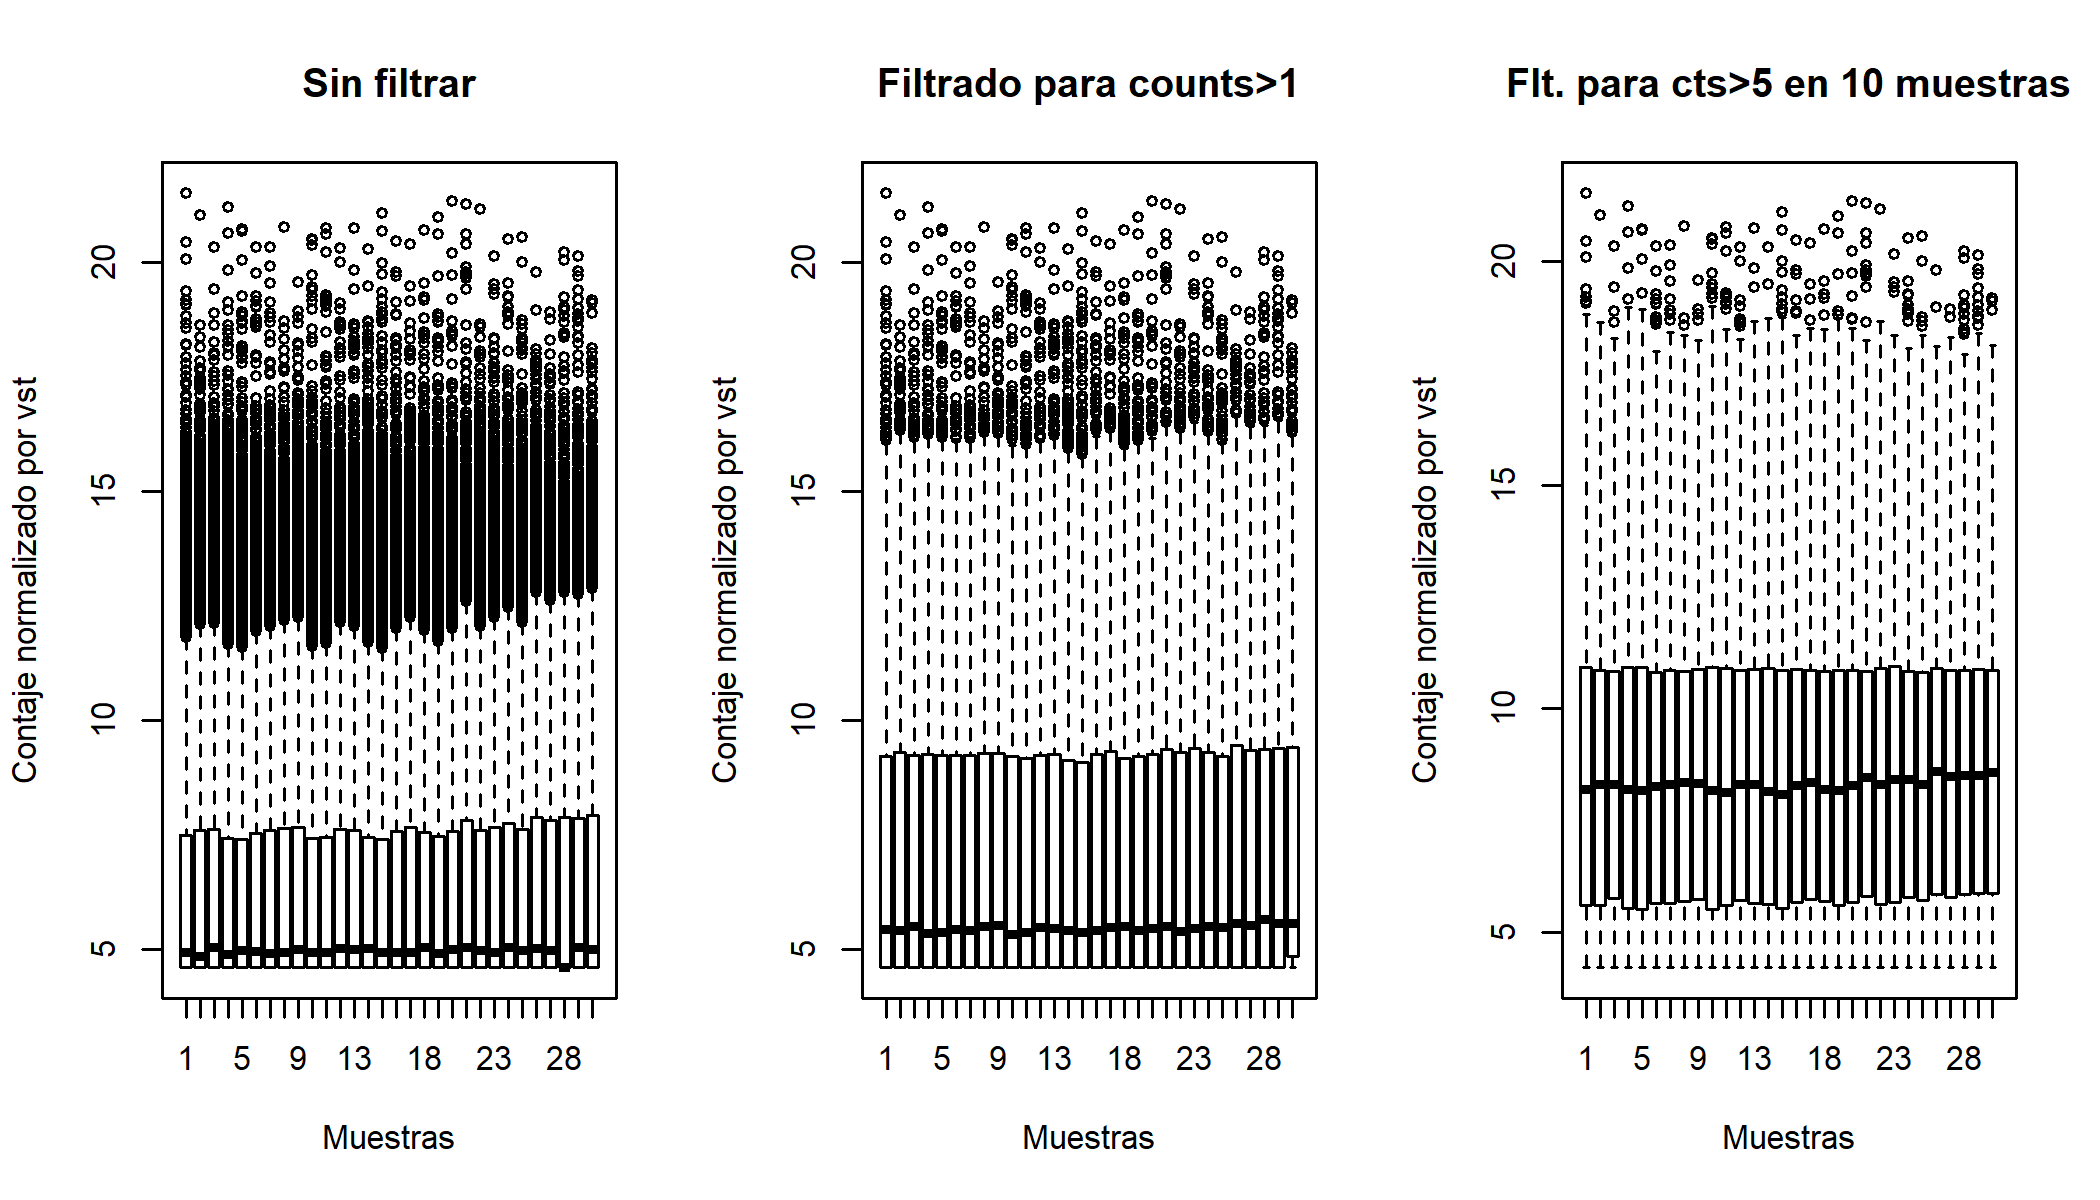
\includegraphics[width=0.8\linewidth]{results/1.Filtraje/1.FiltComp} 

}

\caption{Diagrama de cajas de los contajes de los tránscripts según el filtro aplicado a los datos.}\label{fig:Fig1}
\end{figure}

\begin{figure}

{\centering 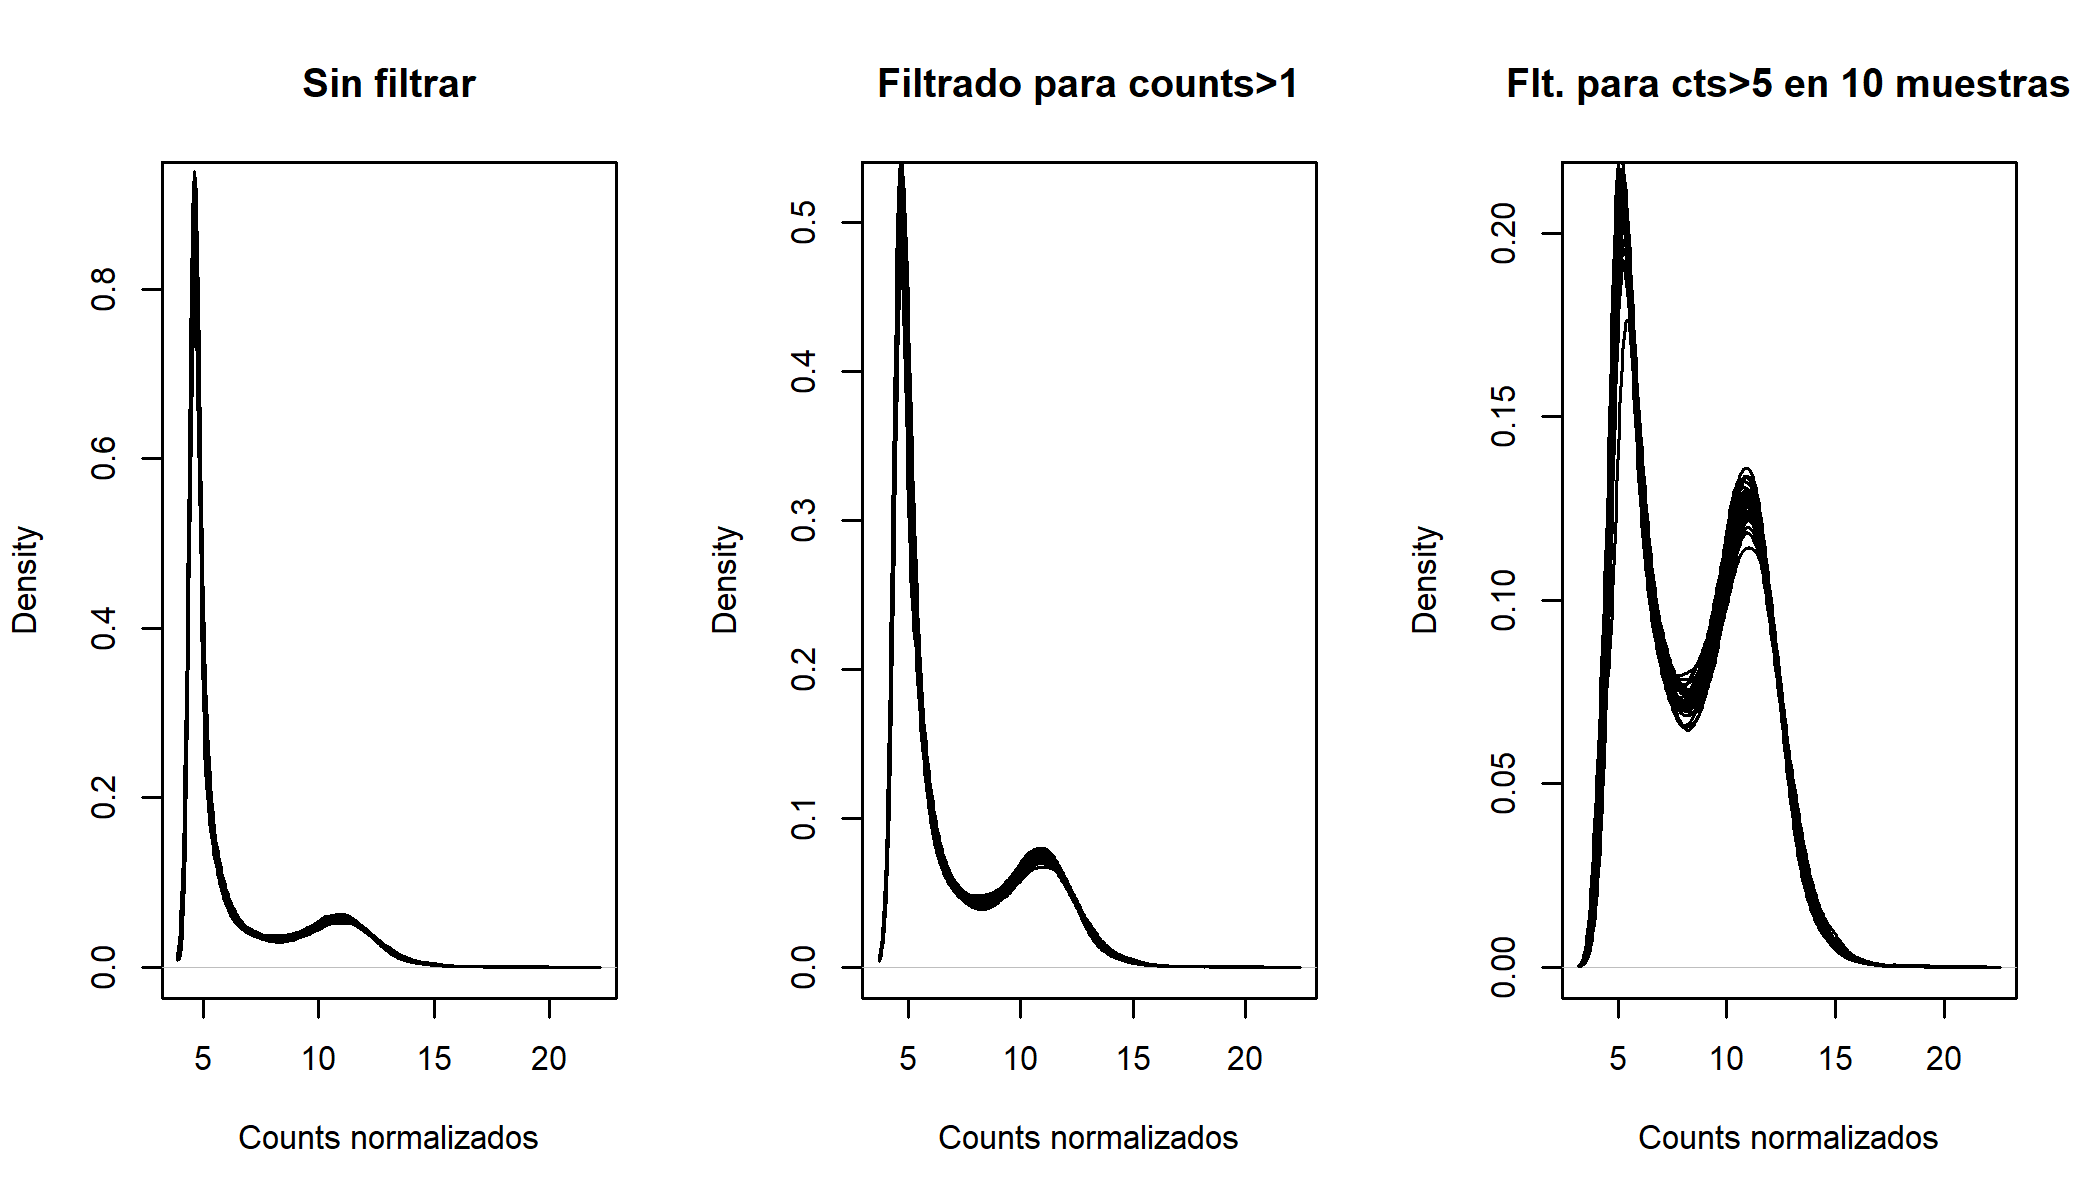
\includegraphics[width=0.8\linewidth]{results/1.Filtraje/2.FiltDens} 

}

\caption{Gráfico de densidad de los contajes de los tránscripts según el filtro aplicado a los datos.}\label{fig:Fig2}
\end{figure}

Aunque a priori el filtro agresivo conserva los datos que podrían ser
interesantes, sin disponer de más detalles biológicos sobre el estudio
(que podrían indicar que los cambios pequeños entre genes pueden, o no,
ser relevantes) se prefiere optar por la opción conservadora. Por esto,
se elige \textbf{un filtro que elimine aquellos tránscripts que no
tienen suficiente información para los contrastes}, es decir, aquellos
que no se han observado en los datos de las muestras o observado una
sola vez (insuficiente para hacer una comparación). Tras el filtrado
básico, el conjunto de datos pasa de \textbf{56202 tránscripts a 43362},
conservando el \(77\%\) de los datos.

\hypertarget{anuxe1lisis-exploratorio}{%
\subsubsection{4.1.3. Análisis
exploratorio}\label{anuxe1lisis-exploratorio}}

Antes de proceder con la identificación de los genes expresados
diferencialmente, puede estudiarse la naturaleza de los datos y las
muestras a través de un análisis descriptivo de estas. Para esto, se
normaliza el número de \emph{counts} por el método VST, que es más
eficiente que \texttt{rlog} cuando hay varias decenas de muestras (y en
este caso, \texttt{n=30}). Para empezar, se representa la distribución
de los \emph{counts} según la muestra con diagramas de cajas y gráfico
de densidad (Figura \ref{fig:Fig3}). Las medias y quantiles
representados en el diagrama de cajas son parecidas para todas las
muestras, y la distribución del gráfico de densidad es prácticamente
identica para todas las muestras, hasta el punto que es imposible
distinguir la línea para cada muestra. Por lo tanto, la composición de
las muestras es similar y se pueden comparar bien con el análisis de
expresión diferencial.

\begin{figure}

{\centering 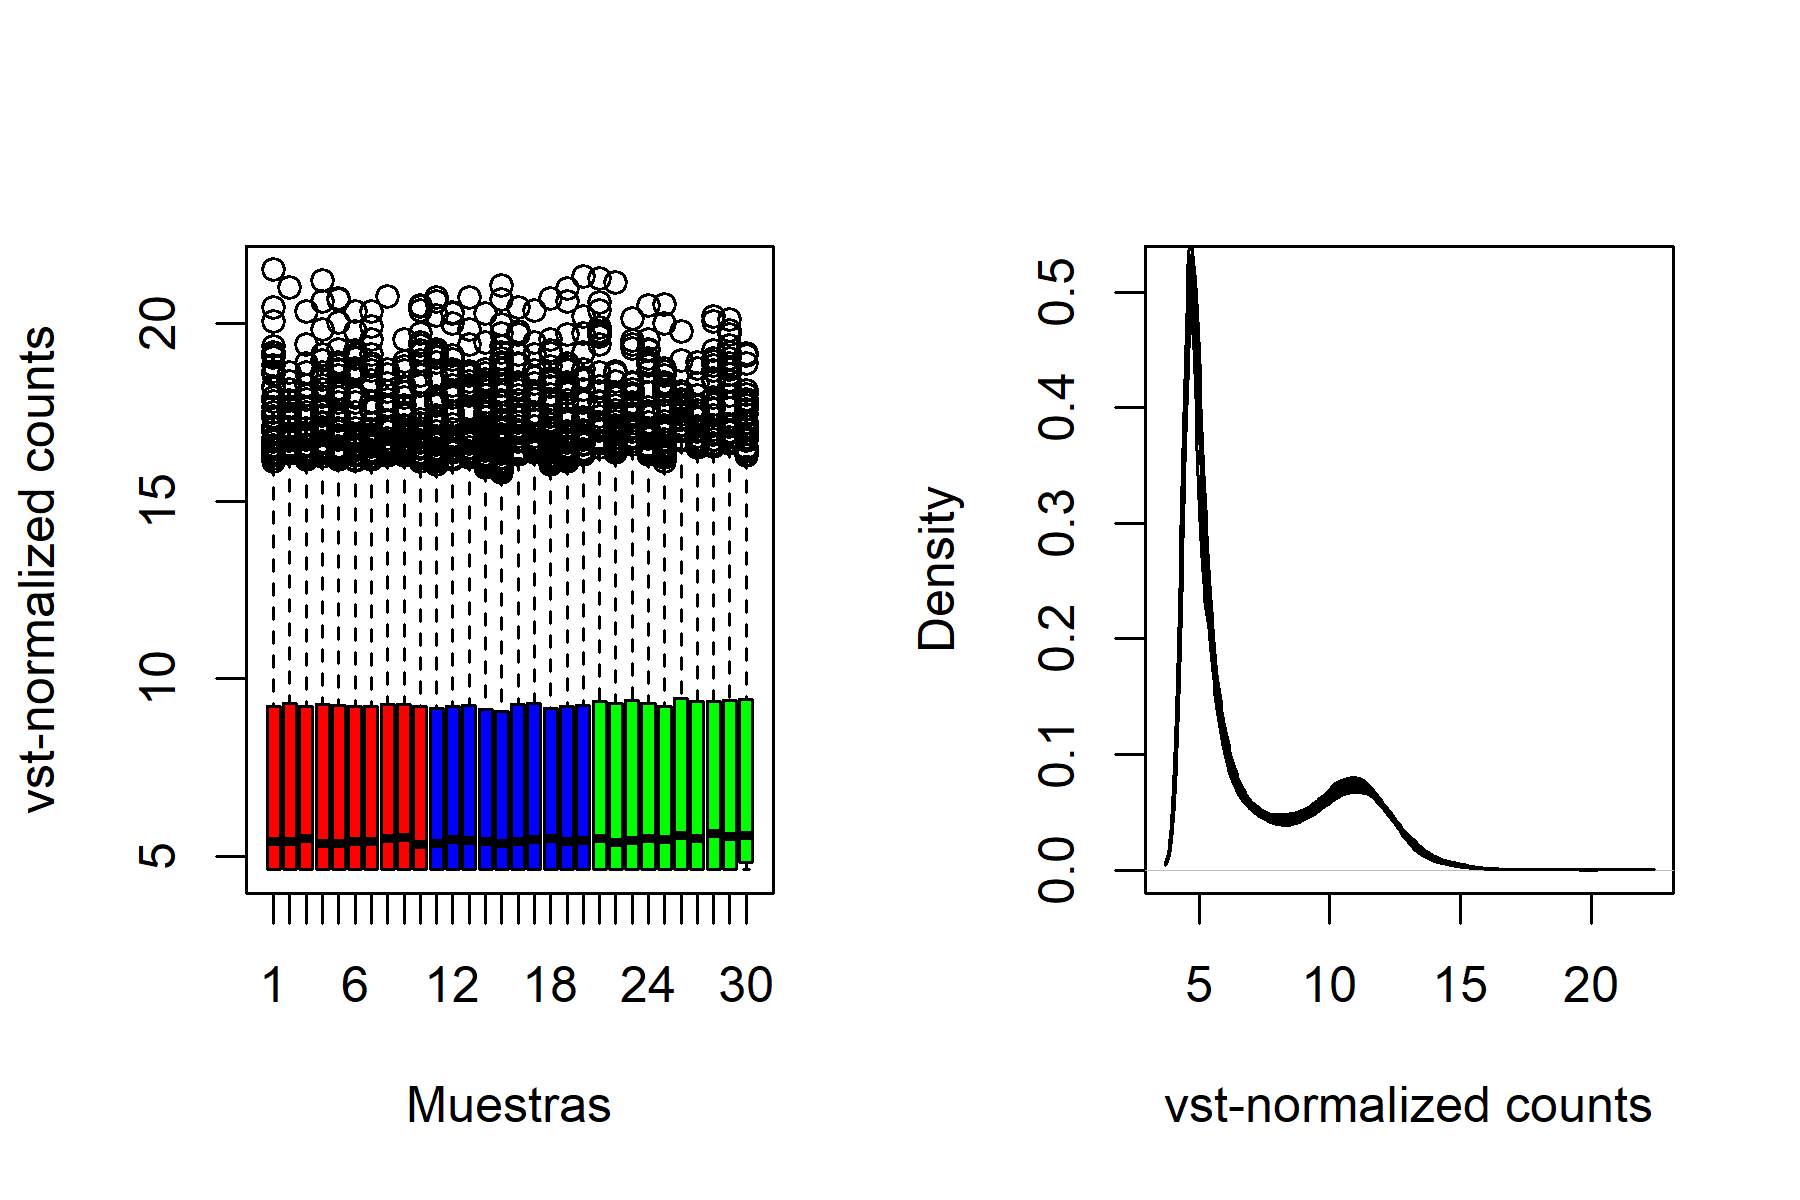
\includegraphics[width=0.8\linewidth]{results/2.AnaDescript/1.CountDist} 

}

\caption{Diagrama de cajas (izquierda) y gráfico de densidad (derecha) de los contajes de cada tránscript normalizados por VST según la muestra. En el diagrama de cajas, las muestras rojas son del grupo NIT, las azules de SFI y las verdes de ELI. }\label{fig:Fig3}
\end{figure}

A continuación, se calculan las distancias entre las muestras según el
número de \emph{counts} de los tránscripts y se representan con un
gráfico de intensidades (\emph{heatmap}). Las muestras más similares o
menos distantes (color más intenso) son aquellas cuyos mismo tránscripts
tienen un valor similar de \emph{counts}, mientras que aquellas más
distantes (color menos intenso) son aquellas cuyos tránscripts más
difieren en el número de \emph{counts}. Además, las muestras se ordenan
según similitud formando clústers (Figura \ref{fig:Fig4}). Si la única
variabilidad entre las muestras fuera dada por el tipo de infiltración o
grupo (NTI/SFI/ELI), entonces se observarían 3 grupos con las 10
muestras correspondientes al mismo tipo. Aún así, en el gráfico se puede
observar que todos los grupos se mezclan entre ellos, almenos en parte.
El grupo que menos se mezcla es el grupo \texttt{ELI}, mientras que las
muestras de \texttt{NIT} y \texttt{SFI} se encuentran mezcladas en gran
parte. Esto indica que hay muestras de grupos distintos que son más
parecidas entre ellas que con muestras de su mismo grupo. La causa
podría ser otro factor de variabilidad de los datos. Aún así, esto no
indica que no se pueda realizar el análisis de expresión diferencial
correctamente, ya que al disponer de 10 muestras de cada grupo es
posible que se puedan identificar patrones de expresión comunes y
característicos de grupo.

\begin{figure}

{\centering 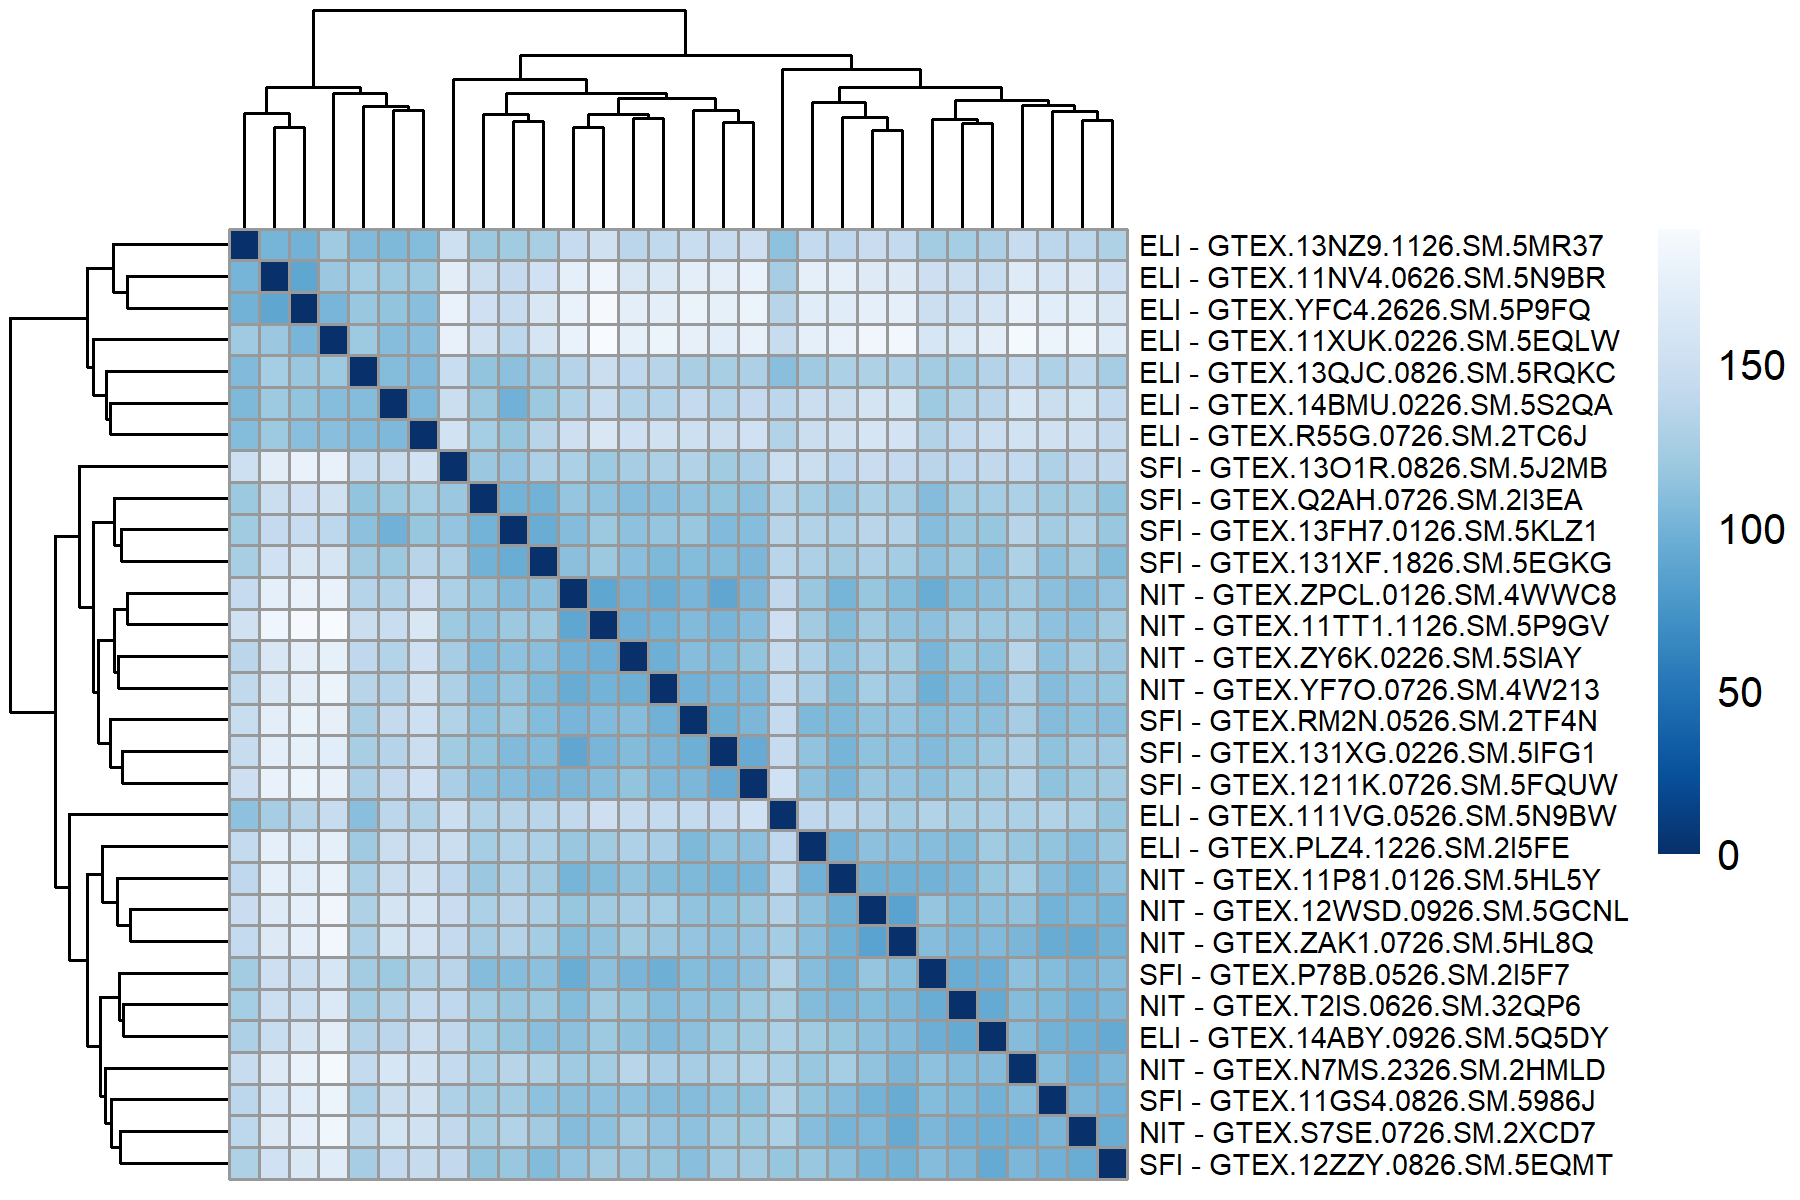
\includegraphics[width=0.8\linewidth]{results/2.AnaDescript/2.DistMuestras_2} 

}

\caption{Matriz de distancias entre las muestras, agrupadas por su similitud. Menor distancia se representa con un azul más oscuro.}\label{fig:Fig4}
\end{figure}

Para profundizar en los factores que podrían causar las diferencias
entre las muestras observadas en el gráfico de similitudes anteriores,
se realiza un análisis de componentes principales (PCA). Los resultados
se representan teniendo en cuenta el grupo (tipo de infiltración) y sexo
del individuo (Figura \ref{fig:Fig5}). Se puede ver que la componente
principal (el factor que explica mayor parte de la varianza) explica
hasta el \(60\%\) de varianza de los datos, mientras que la segunda
componente explica tan solo el \(10\%\) de la varianza.

Al observar la disposición de las muestras en el eje horizontal y según
su color que indica el tipo de infiltración, se puede ver un paralelismo
con los resultados de la matriz de similitudes. Los datos se distribuyen
según el grupo a lo largo del eje horizontal y siguiendo el órden
esperado por el tamaño de las infiltraciones (infiltraciones NIT en un
extremo, ELI en el otro y SFI en el medio). Pese a que esta distribución
presenta algunas excepciones, se podría decir que la primera componente
de la varianza se debe al factor del tipo de infilitración, con lo que
los contrastes planteados seguramente permitirán observar distintos
genes enriquidos según el grupo de infiltración.

En el eje vertical, los datos se distribuyen según el sexo del
individuo. Por lo tanto, la segunda componente se identifica con el
sexo. Como la segunda componente tan solo explica el \(10\%\) de la
varianza, el análisis de los datos se puede realizar teniendo en cuenta
solamente el factor tipo de infiltración, ya que el resto de factores
explicaría menos del \(10\%\) de la varianza. Así pues, el diseño
experimental tenido en cuenta para en análisis será de solo un factor
con tres niveles.

\begin{figure}

{\centering 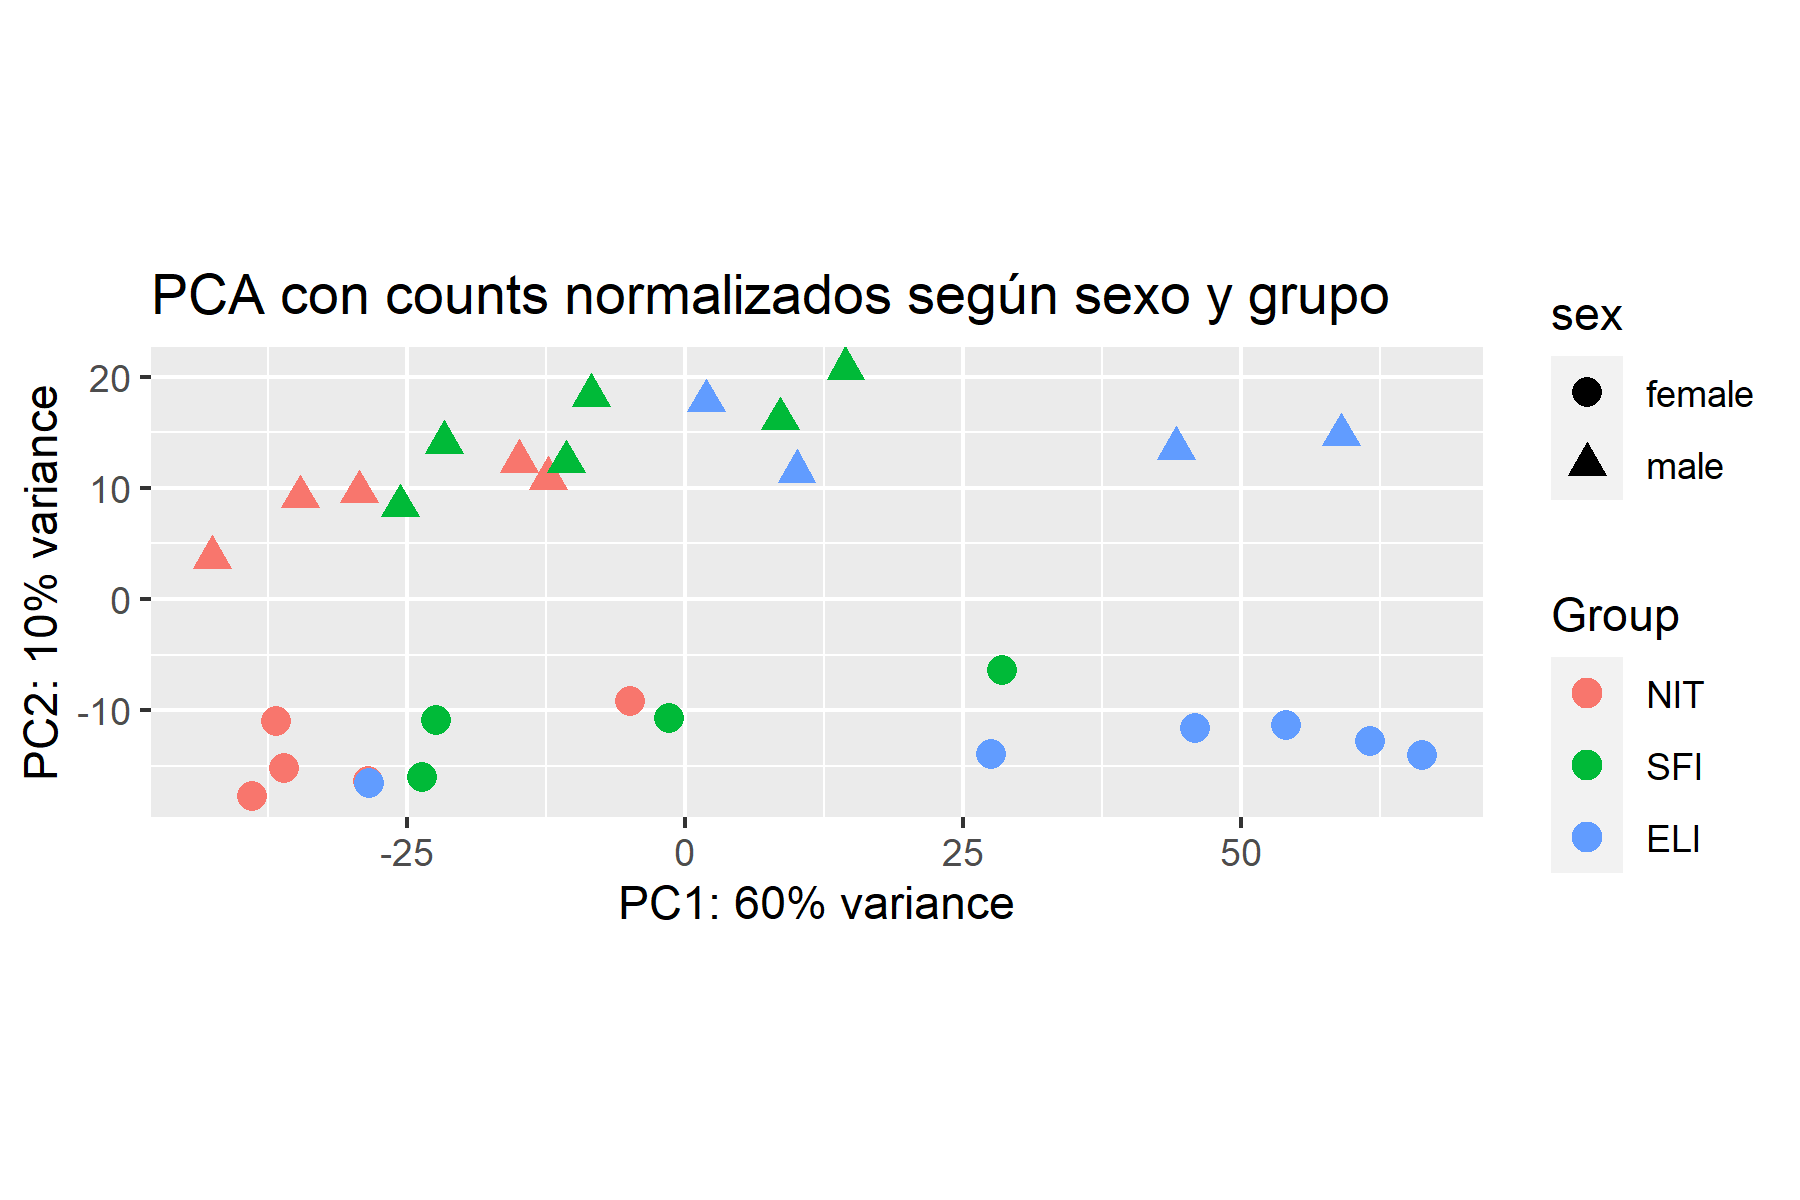
\includegraphics[width=0.8\linewidth]{results/2.AnaDescript/3.PCA} 

}

\caption{Muestras representadas según las dimensiones 1 y 2 de las componentes principales que explican su varianza. La forma de la muestra indica el sexo del individuo y el color el tipo de infiltración.}\label{fig:Fig5}
\end{figure}

\newpage

\hypertarget{identificaciuxf3n-de-genes-expresados-diferencialmente-1}{%
\subsection{4.2. Identificación de genes expresados
diferencialmente}\label{identificaciuxf3n-de-genes-expresados-diferencialmente-1}}

\hypertarget{anuxe1lisis-de-expresiuxf3n-diferencial-1}{%
\subsubsection{4.2.1. Análisis de expresión
diferencial}\label{anuxe1lisis-de-expresiuxf3n-diferencial-1}}

Para entender biológicamente los tipos de infilitración se deben
identificar aquellos genes que se expresan de forma diferencial entre
los tipos de infilitración. El estudio tiene un solo factor con tres
niveles, así que se pueden hacer 3 comparaciones a pares distintas. Para
las comparaciones se tiene en cuenta que los factores están ordenados
según el tamaño de la infiltración. Por lo tanto, el nivel bajo
corresponde a NIT (la clase sin infiltración), el nivel medio a SFI
(infiltración pequeña), y el nivel alto a ELI (infiltración extensa).
Así pues, se definen tres contrastes:

\begin{itemize}
\tightlist
\item
  SFI-NIT: Nivel medio vs.~nivel bajo.
\item
  ELI-NIT: Nivel alto vs.~nivel bajo.
\item
  ELI-SFI: Nivel alto vs.~nivel medio
\end{itemize}

En los tres contrastes, el nivel más alto siempre está como nivel
superior, así que los genes sobre-expresados serán aquellos cuya
expresión incrementa con el tamaño de la infiltración, y los
infra-expresados serán aquellos cuya expresión disminuye con el tamaño
de la infiltración. El órden de los factores se tiene en cuenta al
realizar el análisis de los datos de \emph{RNA-Seq} con \texttt{DESeq}
para asegurar que los resultados reflejan el objetivo a estudiar.

En el proceso de identificación de los genes expresados diferencialmente
se calculan las distancias de Cook entre los \emph{counts}, que se
utilizan para ver si hay alguna muestra que sea un \emph{outlier}. Una
representación con un diagrama de cajas de las distancias de Cook
muestra que ninguna de las muestras es diferente al resto, y por lo
tanto, todas 30 muestras se pueden utilizar para la expresión
diferencial (Figura \ref{fig:Fig6}).

\begin{figure}

{\centering 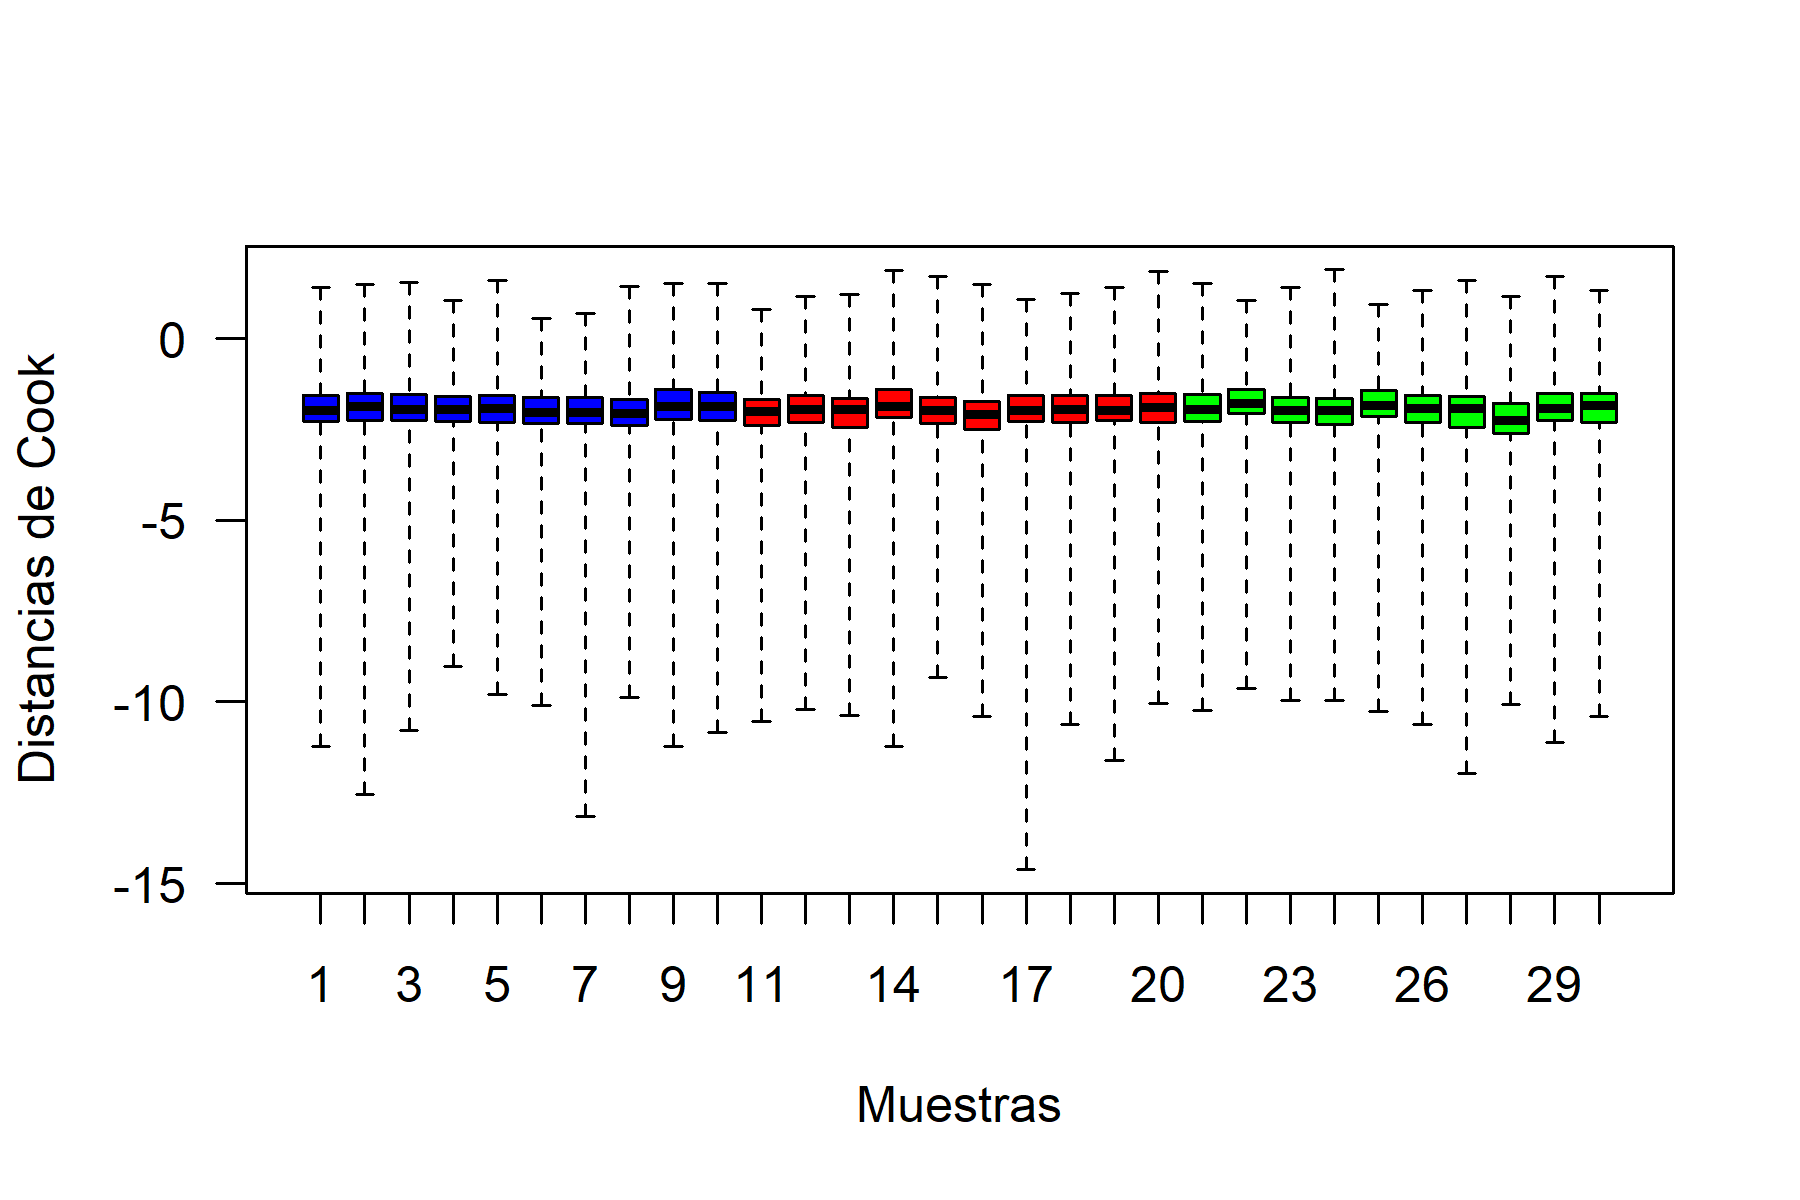
\includegraphics[width=0.8\linewidth]{results/3.ExpresionDiferencial/1.Outl} 

}

\caption{Diagrama de cajas de las distancias de Cook entre los contajes de los tránscripts de cada muestra según el tipo de infiltración (azul, NIT; rojo, SFI; verde, ELI).}\label{fig:Fig6}
\end{figure}

Las comparaciones entre ELI-NIT y ELI-SFI identifican un número mayor
(hasta 1 orden de magnitud mayor) de genes con expresión diferencial (al
\(90\%\) de nivel de confianza) que la comparación SFI-NIT (Tabla 2). En
general, se observan más genes sobre-expresados que infra-expresados en
todas las comparaciones. Nótese que para estas comparaciones no se
aplica un límite mínimo de efecto (Fold Change) para considerar los
genes diferencialmente expresados.

\begin{table}

\caption{\label{tab:unnamed-chunk-2}Resultados de la expresión diferencial de genes en cada comparación.}
\centering
\begin{tabular}[t]{llll}
\toprule
  & SFI.NIT & ELI.NIT & ELI.SFI\\
\midrule
Upregulated & 158 & 4597 & 4582\\
Upregulated (\%) & 0.36\% & 10.6\% & 10.57\%\\
Downregulated & 39 & 2611 & 2732\\
Downregulated (\%) & 0.09\% & 6.02\% & 6.3\%\\
\bottomrule
\end{tabular}
\end{table}

\hypertarget{anotaciuxf3n-de-los-resultados-1}{%
\subsubsection{4.2.2. Anotación de los
resultados}\label{anotaciuxf3n-de-los-resultados-1}}

La anotación de los tránscripts solamente identifica cerca de la mitad
de los tránscripts, habiendo 20860 tránscripts sin anotar. Por esto, al
mostrar los 6 genes con expresión significativa más sobre- e
infra-expresados de cada comparación hay múltiples transcripts sin
identificación y con \texttt{NA} (Tablas 3-8). Aún así, es posible
identificar similitudes entre los contrastes. Por ejemplo, las
comparaciones entre ELI-NIT y ELI-SFI tienen algunos genes sobre- e
infra-expresados en común, indicando que seguramente se tratan de genes
sobre-expresados exclusivamente cuando la infiltración es extensa y
limofóide.

Precisamente estos términos GO tienen que ver con el sistema immunitario
tal y como sugiere el nombre de ELI (extensive lymphoid infiltration),
así que gracias a la anotación se pueden sacar ideas sobre lo que pasa
biológicamente. Aún así, para comparar los tránscripts más comunes es
más apropiado utilizar un diagrama de Venn como se muestra más adelante.

\begin{table}

\caption{\label{tab:unnamed-chunk-3}Genes significativos con mayor infra-expresión del contraste SFI-NIT.}
\centering
\resizebox{\linewidth}{!}{
\begin{tabular}[t]{lrrlll}
\toprule
  & log2FoldChange & padj & symbol & entrez & gname\\
\midrule
ENSG00000254744.3 & -3.004383 & 0.0304654 & NA & NA & NA\\
ENSG00000204603.2 & -2.744411 & 0.0293072 & LINC01257 & 116437 & long intergenic non-protein coding RNA 1257\\
ENSG00000138669.5 & -2.286877 & 0.0390076 & PRKG2 & 5593 & protein kinase cGMP-dependent 2\\
ENSG00000125869.5 & -2.270690 & 0.0720203 & LAMP5 & 24141 & lysosomal associated membrane protein family member 5\\
ENSG00000164488.7 & -2.246964 & 0.0394174 & DACT2 & 168002 & dishevelled binding antagonist of beta catenin 2\\
\addlinespace
ENSG00000075461.5 & -2.202229 & 0.0969815 & CACNG4 & 27092 & calcium voltage-gated channel auxiliary subunit gamma 4\\
\bottomrule
\end{tabular}}
\end{table}

\begin{table}

\caption{\label{tab:unnamed-chunk-3}Genes significativos con mayor sobre-expresión del contraste SFI-NIT.}
\centering
\resizebox{\linewidth}{!}{
\begin{tabular}[t]{lrrlll}
\toprule
  & log2FoldChange & padj & symbol & entrez & gname\\
\midrule
ENSG00000184385.2 & 8.166863 & 0.0051298 & UMODL1-AS1 & 150147 & UMODL1 antisense RNA 1\\
ENSG00000211654.2 & 7.181845 & 0.0644022 & NA & NA & NA\\
ENSG00000211979.2 & 6.484965 & 0.0093955 & NA & NA & NA\\
ENSG00000225972.1 & 6.276841 & 0.0000039 & NA & NA & NA\\
ENSG00000235896.2 & 5.982389 & 0.0093955 & NA & NA & NA\\
\addlinespace
ENSG00000253128.1 & 5.980278 & 0.0047360 & NA & NA & NA\\
\bottomrule
\end{tabular}}
\end{table}

\begin{table}

\caption{\label{tab:unnamed-chunk-3}Genes significativos con mayor infra-expresión del contraste ELI-NIT.}
\centering
\resizebox{\linewidth}{!}{
\begin{tabular}[t]{lrrlll}
\toprule
  & log2FoldChange & padj & symbol & entrez & gname\\
\midrule
ENSG00000110680.8 & -7.262318 & 0.0000011 & CALCA & 796 & calcitonin related polypeptide alpha\\
ENSG00000134443.5 & -5.395689 & 0.0583245 & GRP & 2922 & gastrin releasing peptide\\
ENSG00000250606.4 & -3.774926 & 0.0162834 & NA & NA & NA\\
ENSG00000233491.2 & -3.763374 & 0.0070935 & LOC100128317 & 100128317 & uncharacterized LOC100128317\\
ENSG00000170890.9 & -3.730828 & 0.0092982 & PLA2G1B & 5319 & phospholipase A2 group IB\\
\addlinespace
ENSG00000100604.8 & -3.703757 & 0.0017151 & CHGA & 1113 & chromogranin A\\
\bottomrule
\end{tabular}}
\end{table}

\begin{table}

\caption{\label{tab:unnamed-chunk-3}Genes significativos con mayor sobre-expresión del contraste ELI-NIT.}
\centering
\resizebox{\linewidth}{!}{
\begin{tabular}[t]{lrrlll}
\toprule
  & log2FoldChange & padj & symbol & entrez & gname\\
\midrule
ENSG00000170054.10 & 9.595871 & 0.0000002 & SERPINA9 & 327657 & serpin family A member 9\\
ENSG00000100721.6 & 8.472822 & 0.0000000 & TCL1A & 8115 & T cell leukemia/lymphoma 1A\\
ENSG00000242580.1 & 8.431927 & 0.0000000 & NA & NA & NA\\
ENSG00000211654.2 & 8.325356 & 0.0006198 & NA & NA & NA\\
ENSG00000196092.8 & 8.291902 & 0.0000000 & PAX5 & 5079 & paired box 5\\
\addlinespace
ENSG00000254029.1 & 8.077225 & 0.0076651 & NA & NA & NA\\
\bottomrule
\end{tabular}}
\end{table}

\begin{table}

\caption{\label{tab:unnamed-chunk-3}Genes significativos con mayor infra-expresión del contraste ELI-SFI.}
\centering
\resizebox{\linewidth}{!}{
\begin{tabular}[t]{lrrlll}
\toprule
  & log2FoldChange & padj & symbol & entrez & gname\\
\midrule
ENSG00000110680.8 & -9.533706 & 0.0000000 & CALCA & 796 & calcitonin related polypeptide alpha\\
ENSG00000134443.5 & -7.784920 & 0.0030604 & GRP & 2922 & gastrin releasing peptide\\
ENSG00000100604.8 & -5.820203 & 0.0000001 & CHGA & 1113 & chromogranin A\\
ENSG00000232111.1 & -5.130430 & 0.0007519 & NA & NA & NA\\
ENSG00000157005.3 & -4.939395 & 0.0000590 & SST & 6750 & somatostatin\\
\addlinespace
ENSG00000105388.10 & -3.945724 & 0.0011874 & CEACAM5 & 1048 & CEA cell adhesion molecule 5\\
\bottomrule
\end{tabular}}
\end{table}

\begin{table}

\caption{\label{tab:unnamed-chunk-3}Genes significativos con mayor sobre-expresión del contraste ELI-SFI.}
\centering
\resizebox{\linewidth}{!}{
\begin{tabular}[t]{lrrlll}
\toprule
  & log2FoldChange & padj & symbol & entrez & gname\\
\midrule
ENSG00000162897.10 & 7.601415 & 0.0000055 & FCAMR & 83953 & Fc fragment of IgA and IgM receptor\\
ENSG00000213231.8 & 6.728051 & 0.0000021 & TCL1B & 9623 & T cell leukemia/lymphoma 1B\\
ENSG00000257275.2 & 5.994352 & 0.0008257 & NA & NA & NA\\
ENSG00000258878.1 & 5.877264 & 0.0000193 & NA & NA & NA\\
ENSG00000250850.2 & 5.819245 & 0.0000000 & NA & NA & NA\\
\addlinespace
ENSG00000100721.6 & 5.683927 & 0.0000002 & TCL1A & 8115 & T cell leukemia/lymphoma 1A\\
\bottomrule
\end{tabular}}
\end{table}

\hypertarget{representaciuxf3n-gruxe1fica}{%
\subsubsection{4.2.3. Representación
gráfica}\label{representaciuxf3n-gruxe1fica}}

Los \emph{counts} de un tránscript de interés pueden visualizarse en
cada muestra clasificada según el tipo de infiltración. Nótese que los
\emph{counts} se muestran normalizados con la normalización aplicada
automáticamente por \texttt{DESeq2} para el contraste. Como ejemplo se
han selecionado dos tránscripts de interés, identificados como
ENSG00000100721.6 (del gen \emph{T cell leukemia/lymphoma}, TCL1A) y
ENSG00000100604.8 (del gen \emph{chromogranin A}, CHGA) y representado
el número de \emph{counts} de cada uno según la muestra (Figura
\ref{fig:Fig7}). El primero de estos se encuentra entre los genes más
infra-expresados de las comparaciones ELI-NIT y ELI-SFI pero no en la
comparación SFI-NIT. El gráfico concuerda con esta información, ya que
se vé que los \emph{counts} de este tránscript en las muestras de ELI
son más elevadas que en el resto de muestras. Aún así, hay algunas
muestras de ELI cuyo valor no es tan alto y los gráficos no permiten
saber si esta expresión es significativa, por lo que solamente sirven de
soporte para el análisis de expresión diferencial.

En el caso del otro tránscript estudiado, ENSG00000100604.8, se
encuentra infra-expresado en los contrastes ELI-NIT y ELI-SFI, pero no
entre SFI-NIT. La misma información se puede ver en el gráfico, ya que
los counts de NIT y SFI son más elevados que en ELI, por lo que se
encuentra infra-expresado en ELI. De nuevo, la dispersión de las
muestras es grande entre NIT y SFI y es el contraste estadístico el que
indica que este gen es significativamente infra-expresado en ELI.

\begin{figure}

{\centering 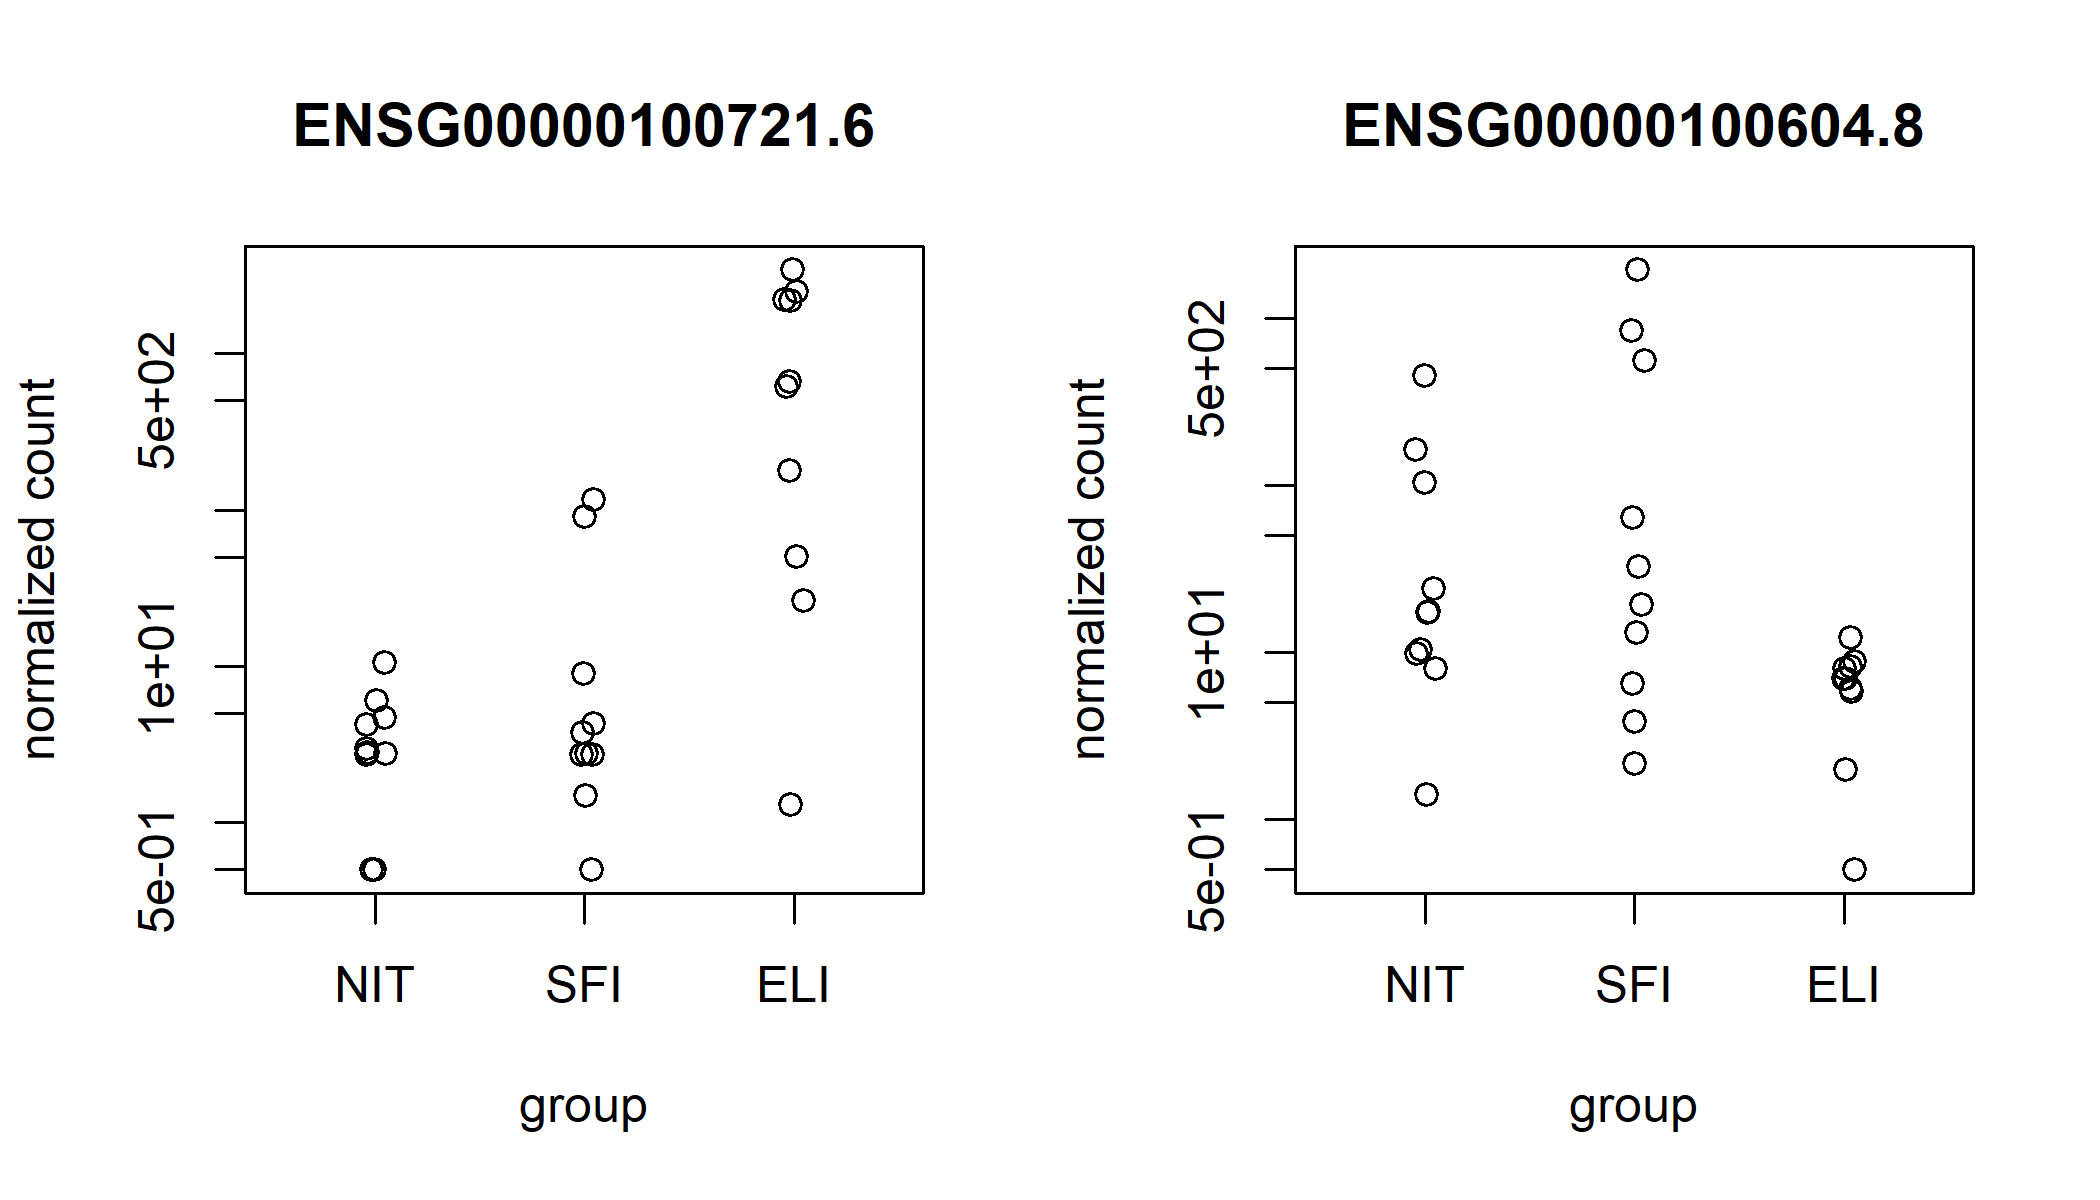
\includegraphics[width=0.8\linewidth]{results/4.DEAnl/1.CntsTOP} 

}

\caption{Contaje de un tránscript sobre-expresado (izquierda) y otro infra-expresado (derecha) en ELI de cada muestra según el tipo de infiltración.}\label{fig:Fig7}
\end{figure}

Estos gráficos también pueden crearse para visualizar un conjunto
determinado de tránscripts individualmente. A continuación se muestran
los 6 tránscripts con mayor sobre-expresión y significativos al \(90\%\)
de confianza del contraste ELI-NIT (también mostrados en la Tabla 6). En
todos los casos se puede ver que los niveles de algunas muestras de ELI
son muy elevados mientras que el nivel en NIT es bajo (Figura
\ref{fig:Fig8}). Como en este contraste no se tiene en cuenta la muestra
SFI, hay algunos tránscripts cuyo nivel en SFI es alto y otros cuyo
nivel es bajo.

\begin{figure}

{\centering 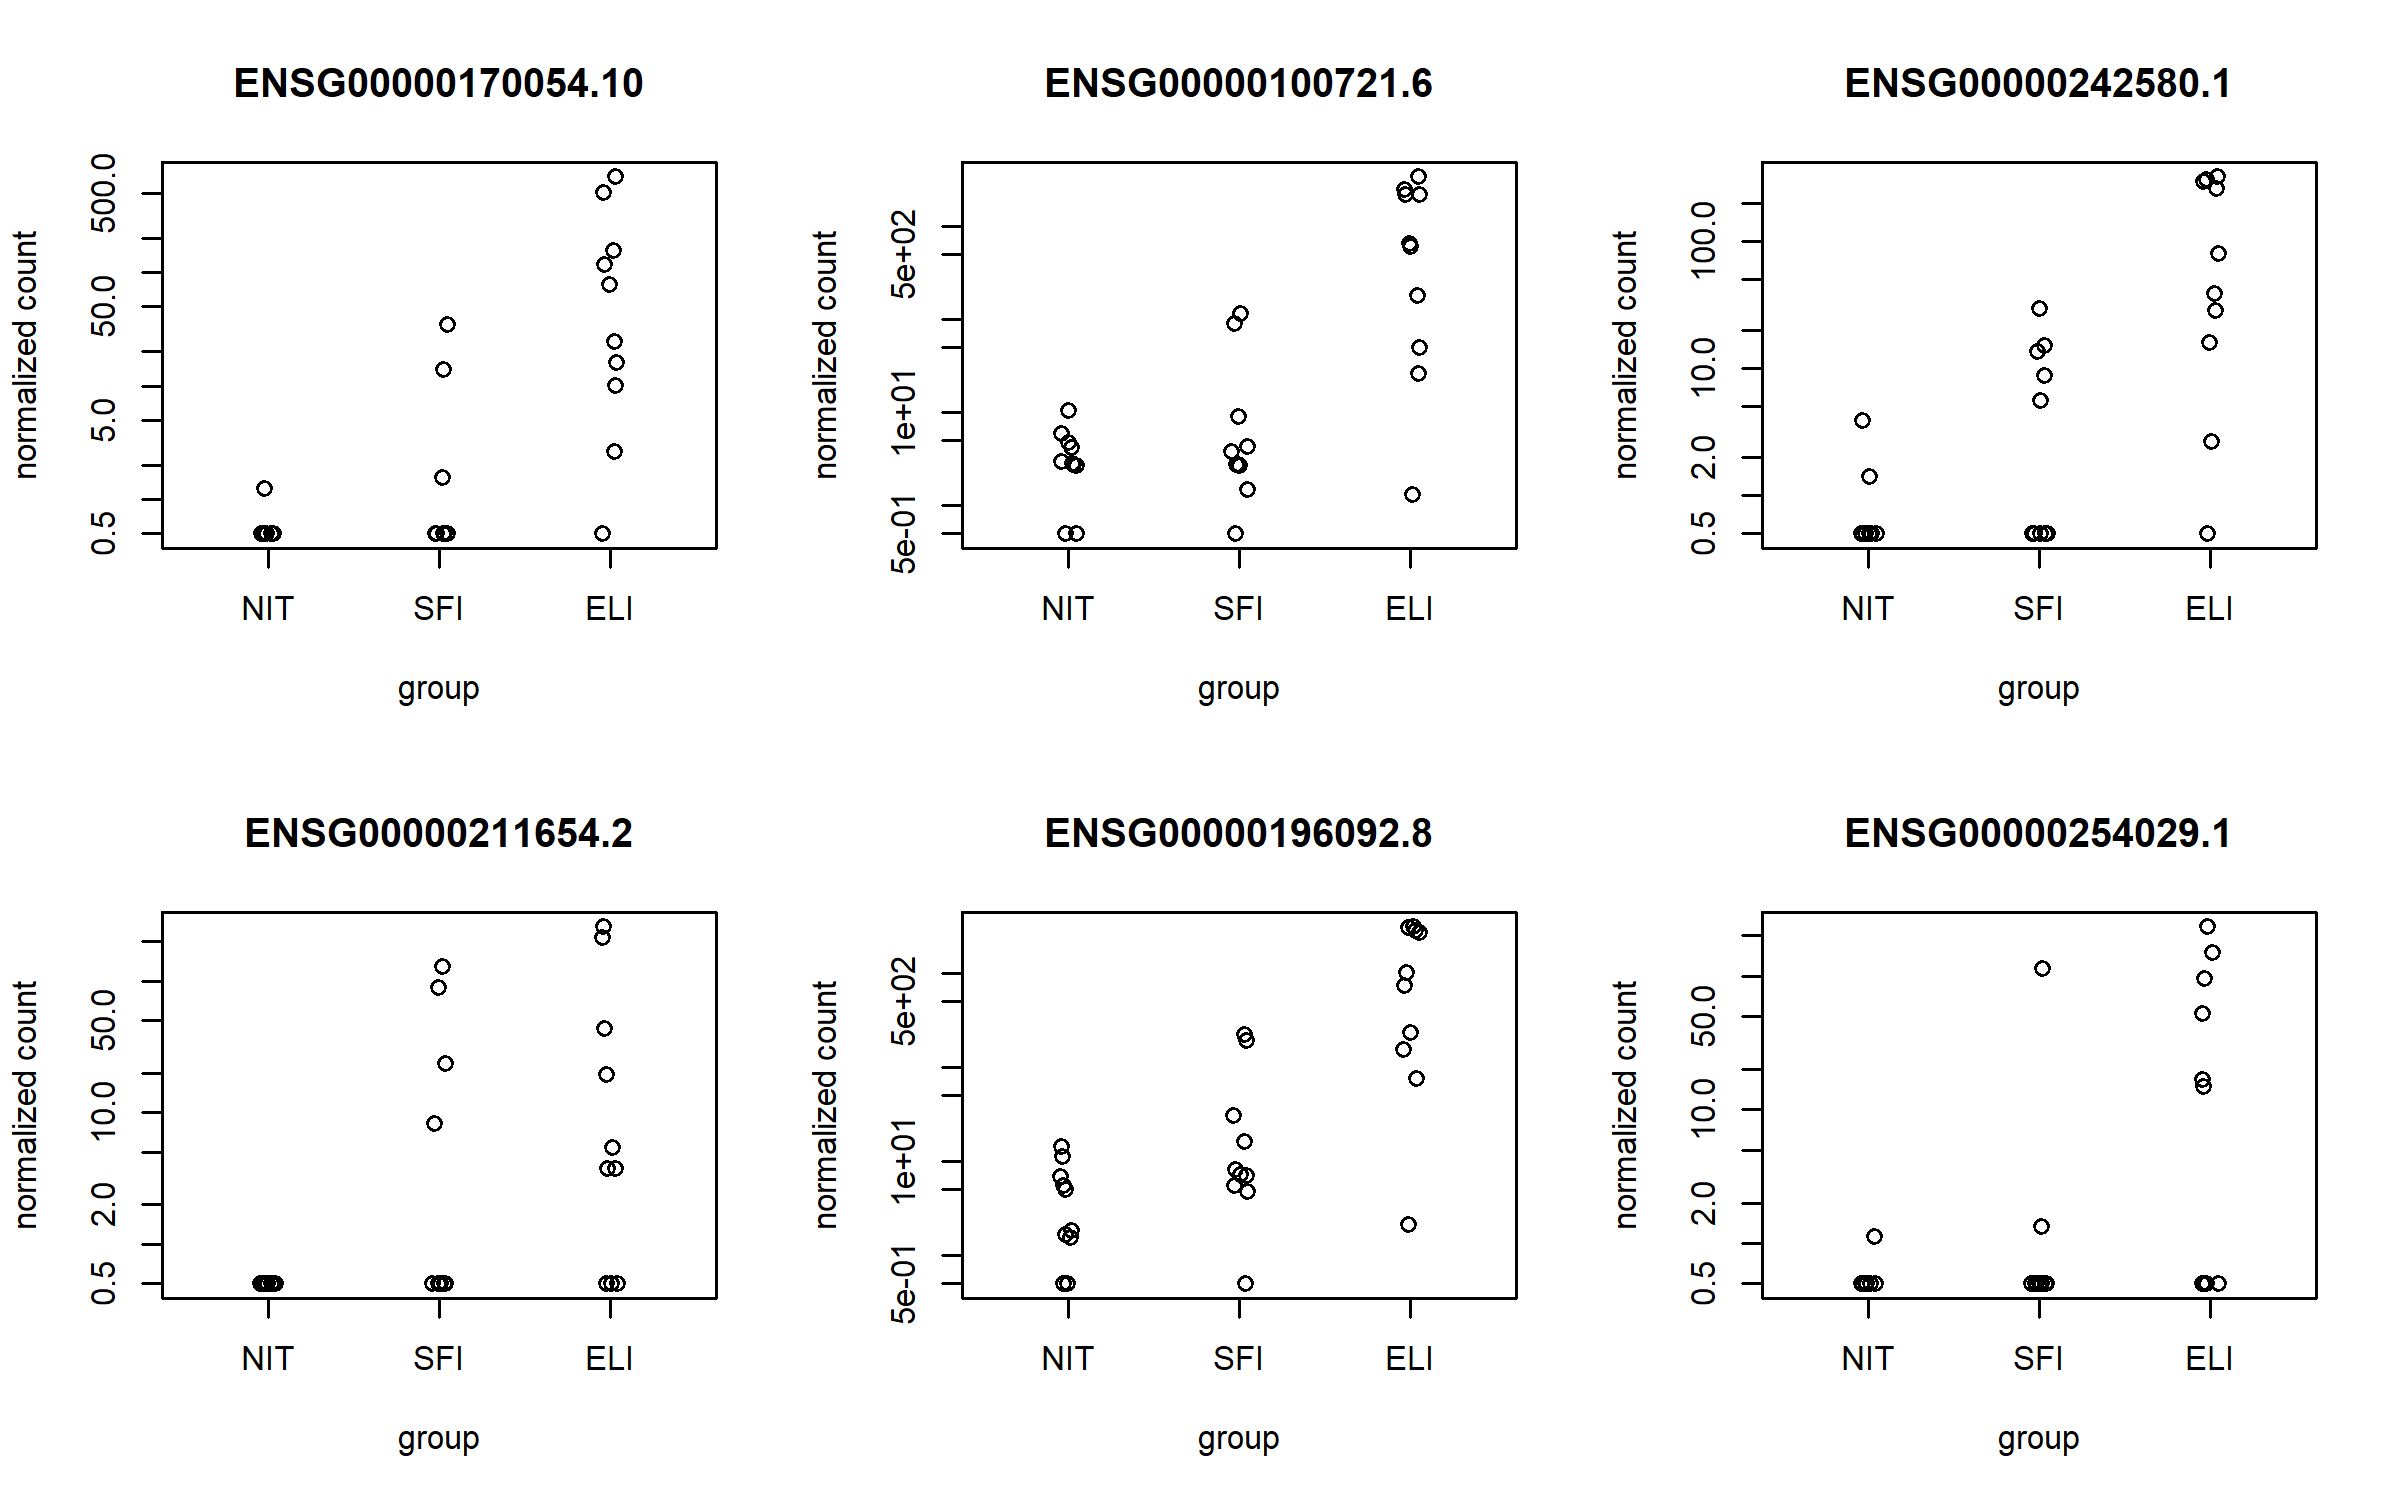
\includegraphics[width=0.8\linewidth]{results/4.DEAnl/2.CntsEvN} 

}

\caption{Contaje de los 6 tránscripts con mayor sobre-expresión en el contraste ELI-NIT de cada muestra según el tipo de infiltración.}\label{fig:Fig8}
\end{figure}

Para visualizar las diferencias entre las muestras contrastadas para
cada uno de los tránscripts analizados se utilizan gráficos MA. Los
tránscripts se distribuyen en el eje horizontal (A) según el valor medio
de \emph{counts} del tránscript en el conjunto de las muestras, y en el
eje vertical (M) según el efecto (\emph{log fold change}) de este
tránscript en el contraste. Como ejemplo, se muestran los gráficos MA de
los contrastes SFI-NIT y ELI-NIT para ver como se pueden utilizar para
comparar la distribución de las comparaciones (Figuras \ref{fig:Fig9} y
\ref{fig:Fig10}).

De entrada, se puede ver que los datos están bien normalizados en las
dos muestras porque la mayoría de tránscripts tienen el valor cero en el
eje vertical. Esto es así porqué la mayoría de tránscripts no tiene un
nivel de expresión diferente entre las muestras y por lo tanto su efecto
(\emph{log fold change}) debe ser cero, tal y como se vé en el eje
vertical. En los dos gráficos MA se muestra la posición del gen con
menor \emph{p-valor} ajustado. En ambos casos, corresponde a un gen
sobre-expresado ya que el valor del eje vertical es mayor que cero
porqué su efecto (\emph{log fold change}) es positivo. También en ambos
casos el gen con mayor \emph{p-valor} ajustado no corresponde al que
tiene mayor efecto entre los genes.

Al comparar los gráficos entre los contrastes SFI-NIT y ELI-NIT se puede
ver que hay más tránscripts con efecto (que se desvian de \emph{log fold
change}=0) entre ELI-NIT que entre SFI-NIT, tal y como se ha podido ver
al realizar los contrastes y encontrar un porcentaje mayor de
tránscripts expresados con significancia en la comparación ELI-NIT
(Tabla 2).

\begin{figure}

{\centering 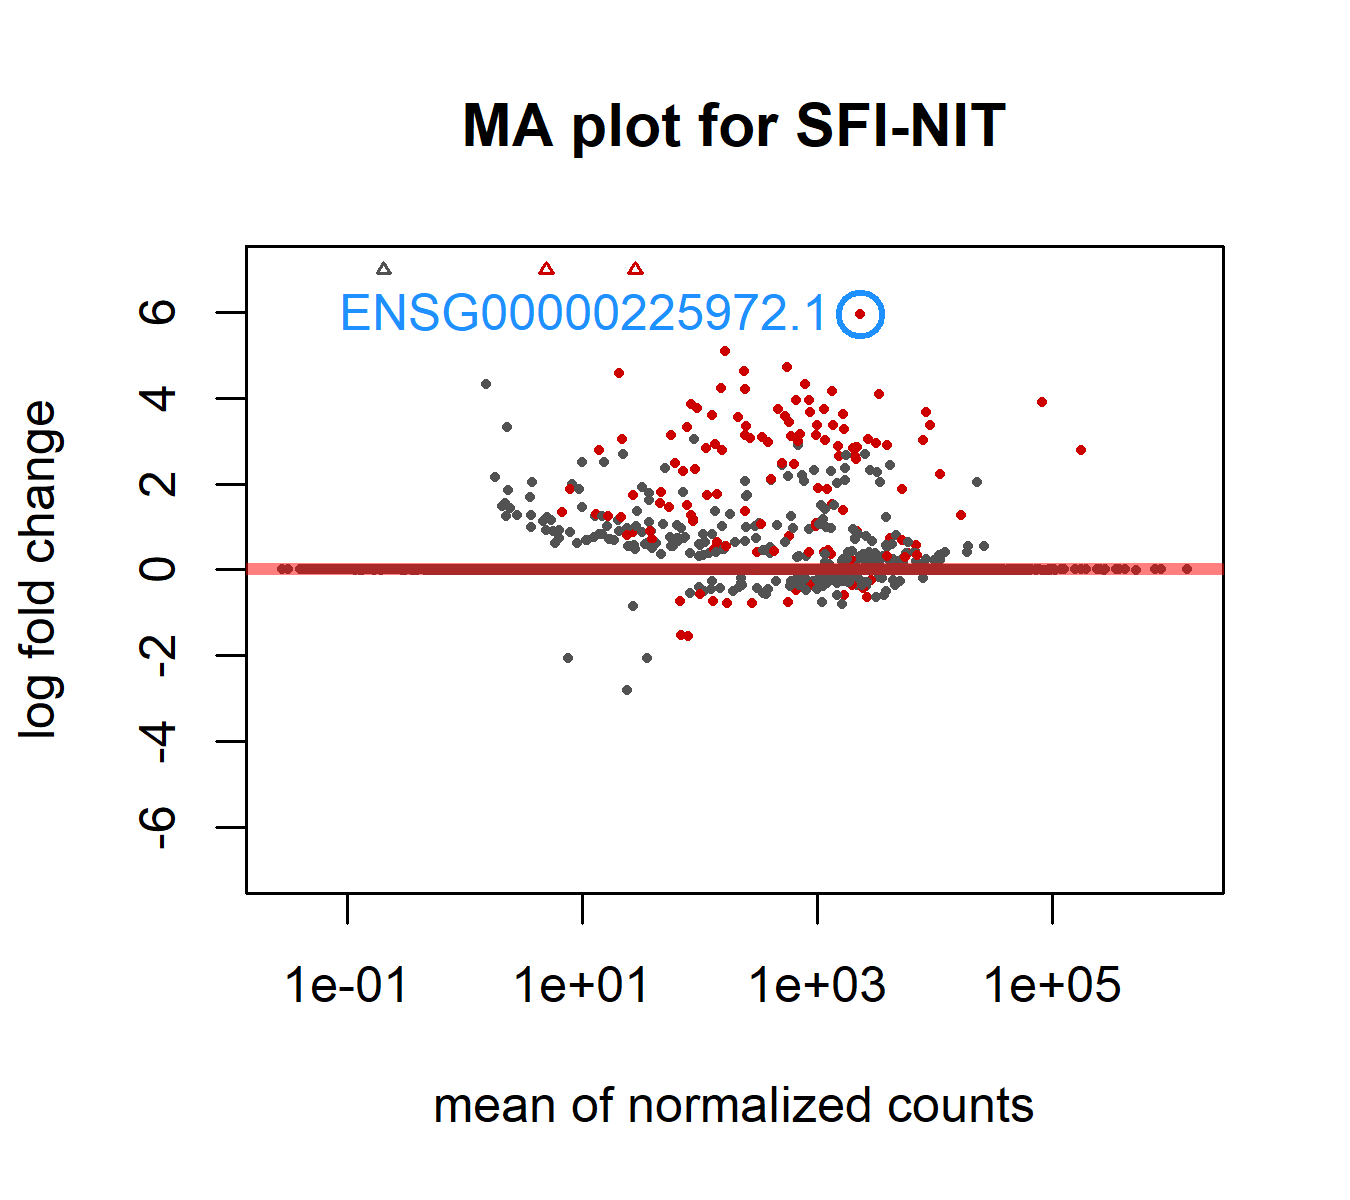
\includegraphics[width=0.8\linewidth]{results/4.DEAnl/3.MASvN_2} 

}

\caption{Gráfico MA de la comparación SFI-NIT, mostrando los tránscripts según su efecto (log fold change) y los counts medios (eje horizontal). Los triangulos corresponden a tránscripts fuera del rango del eje vertical. Se muestra la identidad del tránscript con menor p-valor ajustado.}\label{fig:Fig9}
\end{figure}

\begin{figure}

{\centering 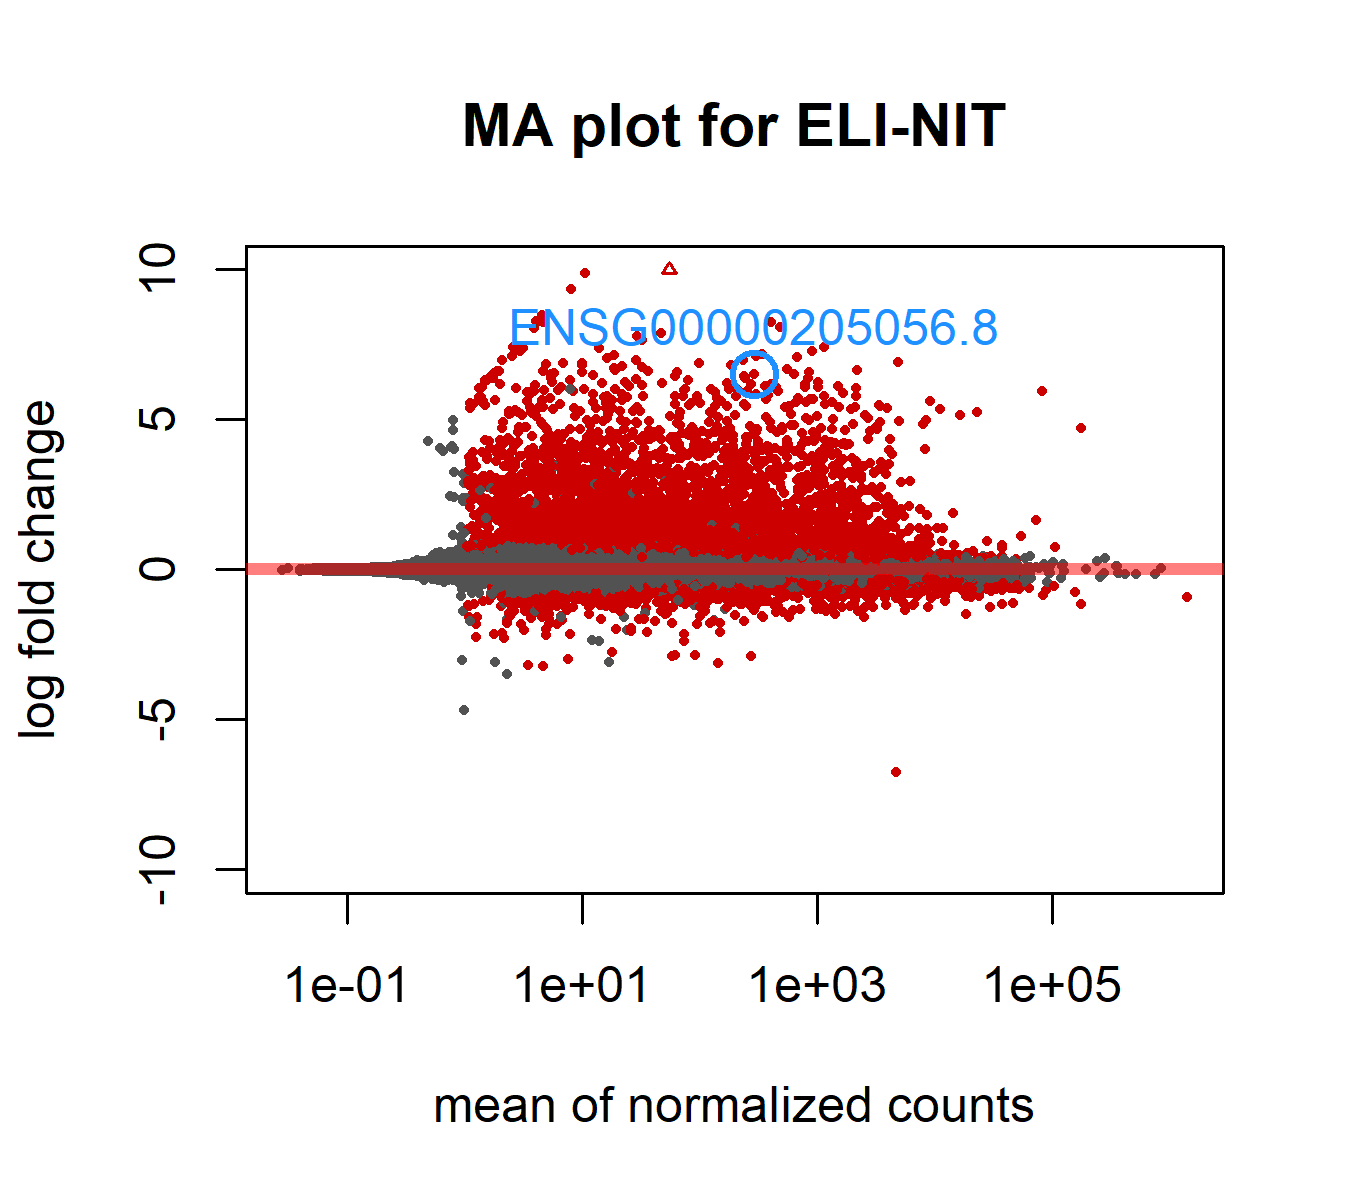
\includegraphics[width=0.8\linewidth]{results/4.DEAnl/4.MAEvN_2} 

}

\caption{Gráfico MA de la comparación ELI-NIT, mostrando los tránscripts según su efecto (log fold change) y los counts medios (eje horizontal). Los triangulos corresponden a tránscripts fuera del rango del eje vertical. Se muestra la identidad del tránscript con menor p-valor ajustado.}\label{fig:Fig10}
\end{figure}

Los resultados del análisis de expresión diferencial pueden utilizarse
para crear grupos entre los tránscripts con patrones de expresión
similar y entre muestras. Para ello, se seleccionan los 20 genes con más
expresión diferencial entre las muestras estudiadas y se representan por
grupos. Nótese que se utilizan los \emph{counts} normalizados por VST.
En el \emph{heatmap} resultante puede verse como se forman grupos entre
los tránscripts que siguen un patrón común en varias de las muestras
(Figura \ref{fig:Fig11}). En la parte superior se identificada cada
muestra según el sexo y el tipo de infiltración. Los grupos creados
según el tipo de infiltración contienen desviaciones respeto las
identidades de las muestras, seguramente causadas por mirar solamente un
conjunto pequeño de genes. Sorprendentemente, hay algunos patrones
génicos que parecerían correlacionarse mejor con el sexo que con el tipo
de infiltración.

\begin{figure}

{\centering 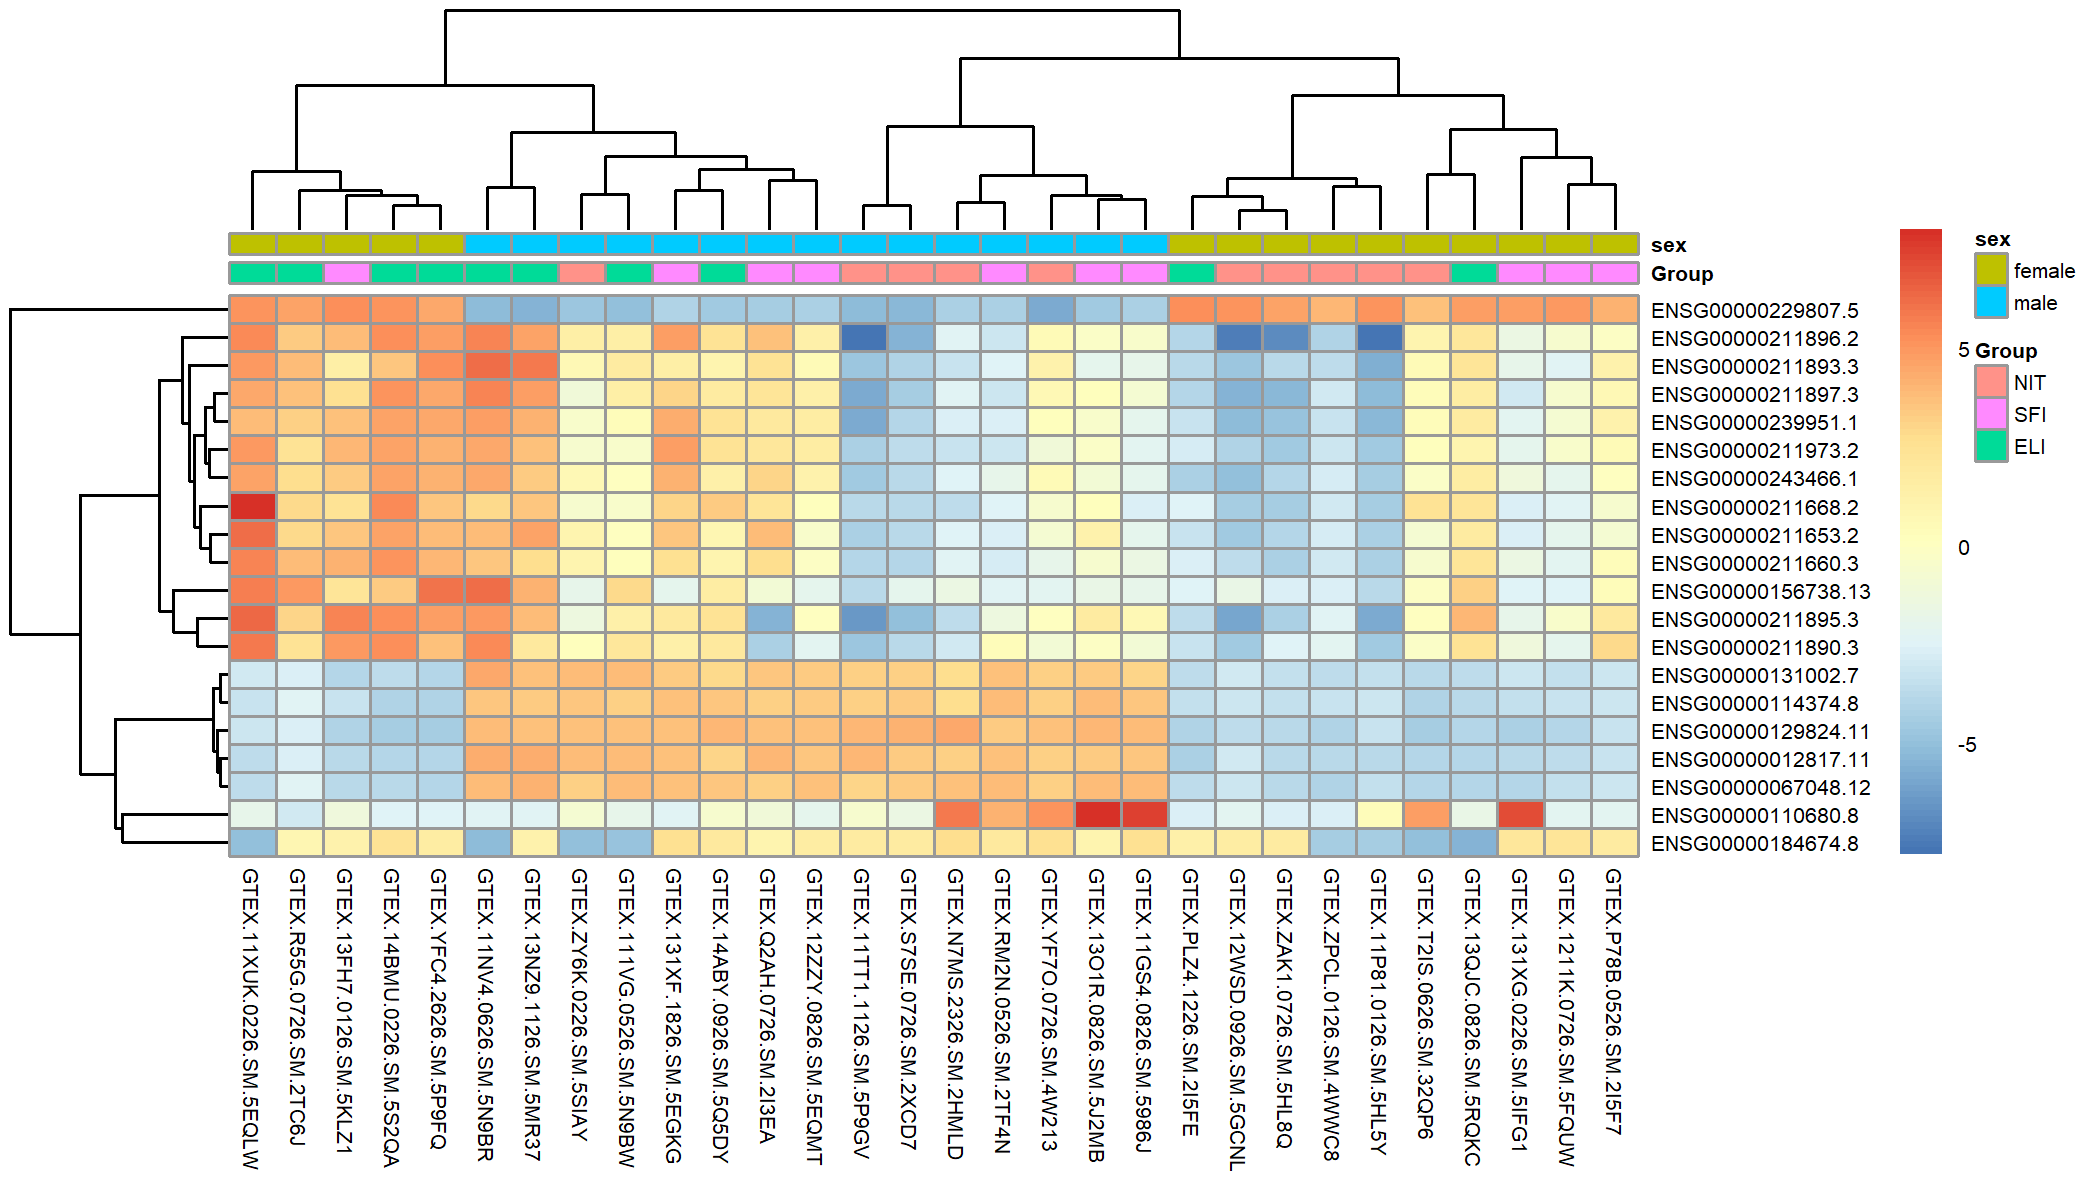
\includegraphics[width=0.8\linewidth]{results/4.DEAnl/5.Heatmap_2} 

}

\caption{Matriz de intensidades (heatmap) que indica las correlaciones entre la expresión de los 20 tránscripts (eje vertical) con mayor variabilidad entre las muestras (eje horizontal). Se agrupan los tránscripts, y también las muestras según sexo y tipo de infiltración. Cuando mayor sobre-expresión hay entre la comparación mayor es la intensidad del color rojo, mientras que para infra-expresión se utiliza el color azul.}\label{fig:Fig11}
\end{figure}

Finalmente, pueden representarse los resultados de expresión diferencial
pueden representarse en un \emph{Volcano Plot} para comparación. El
\emph{volcano plot} representa los tránscripts según su
\texttt{log2FoldChange} que indica el nivel y tipo del efecto y según su
\emph{p-valor} ajustado que indica la significancia de este cambio. El
\emph{volcano plot} de la comparación ELI-NIT muestra una mayor
variabilidad en los valores de efecto de los genes sobre-expresados que
los infra-expresados (Figura \ref{fig:Fig12}).

\begin{figure}

{\centering 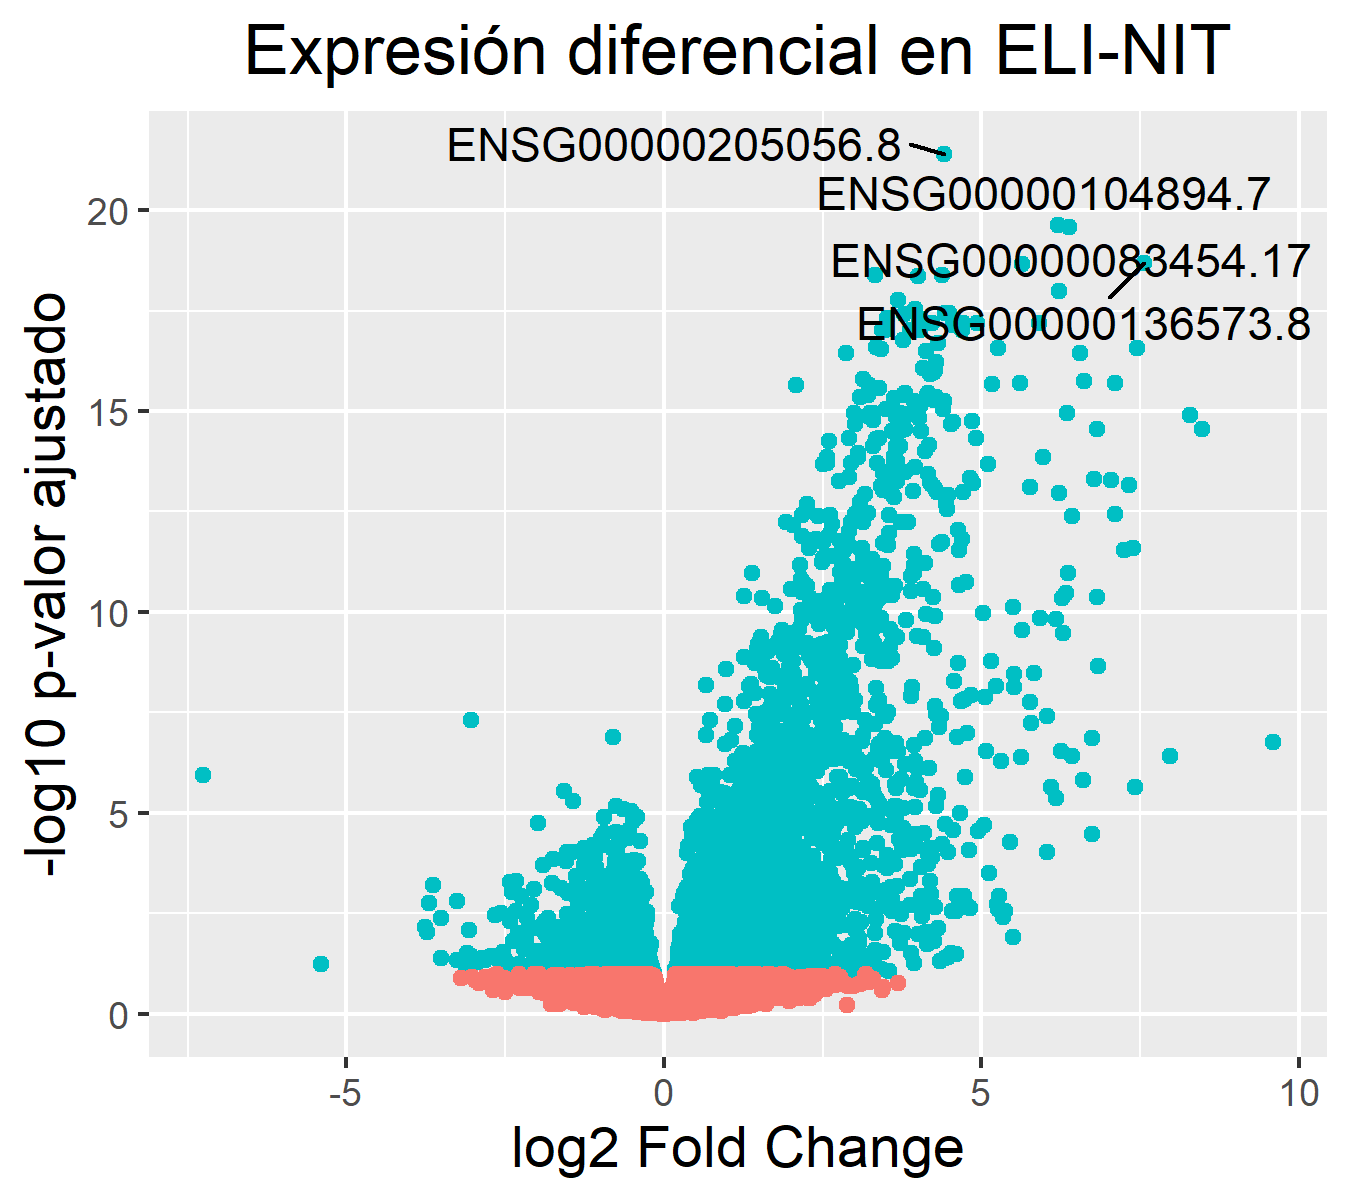
\includegraphics[width=0.8\linewidth]{results/4.DEAnl/6.VolcPl} 

}

\caption{Volcano plot de los tránscripts de la comparación ELI-NIT. Se muestra el Ensembl ID de los 4 tránscripts con menor p-valor ajustado. Los tránscripts cuyo p-valor es inferior a 0.1 se muestran de color rojo, así que los tránscripts azules son los tránscripts significantes.}\label{fig:Fig12}
\end{figure}

\hypertarget{comparaciones-muxfaltiples-1}{%
\subsection{4.3. Comparaciones
múltiples}\label{comparaciones-muxfaltiples-1}}

Para profundizar en los detalles de los tránscripts de interés es
necesario comparar las distintas comparaciones a pares entre ellas. Para
ello, se utilizan diagramas de Venn, que muestra el número de genes en
común entre los contrastes y según si son sobre- o infra-expresados
(Figura \ref{fig:Fig13}). Nótese que se consideran los tránscripts
significativos al \(90\%\) de nivel de confianza y no hay un límite
mínimo de efecto (si \texttt{log2FoldChange\textgreater{}0} es
sobre-expresado, y si \texttt{log2FoldChange\textless{}0} es
infra-expresado).

El diagrama de Venn muestra patrones interesantes, como que un número
elevado de tránscripts (\(3247+1296\)) presentan una regulación parecida
entre las comparaciones ELI-NIT y ELI-SFI. Estos genes en común son
aquellos cuya expresión es más elevada o baja en ELI que en el resto de
grupos. Hay un número menor de tránscripts (\(97\)) con el mismo
comportamiento entre ELI-NIT y SFI-NIT, que corresponden a aquellos
genes que presentan una expresión más elevada o baja tanto en ELI como
SFI pero no en NIT. Es logico observar que no hay genes con el mismo
patrón de expresión diferencial entre SFI-NIT y ELI-SFI, ya que una de
las comparaciones utiliza SFI como nivel alto y la otra como nivel bajo.

\begin{figure}

{\centering 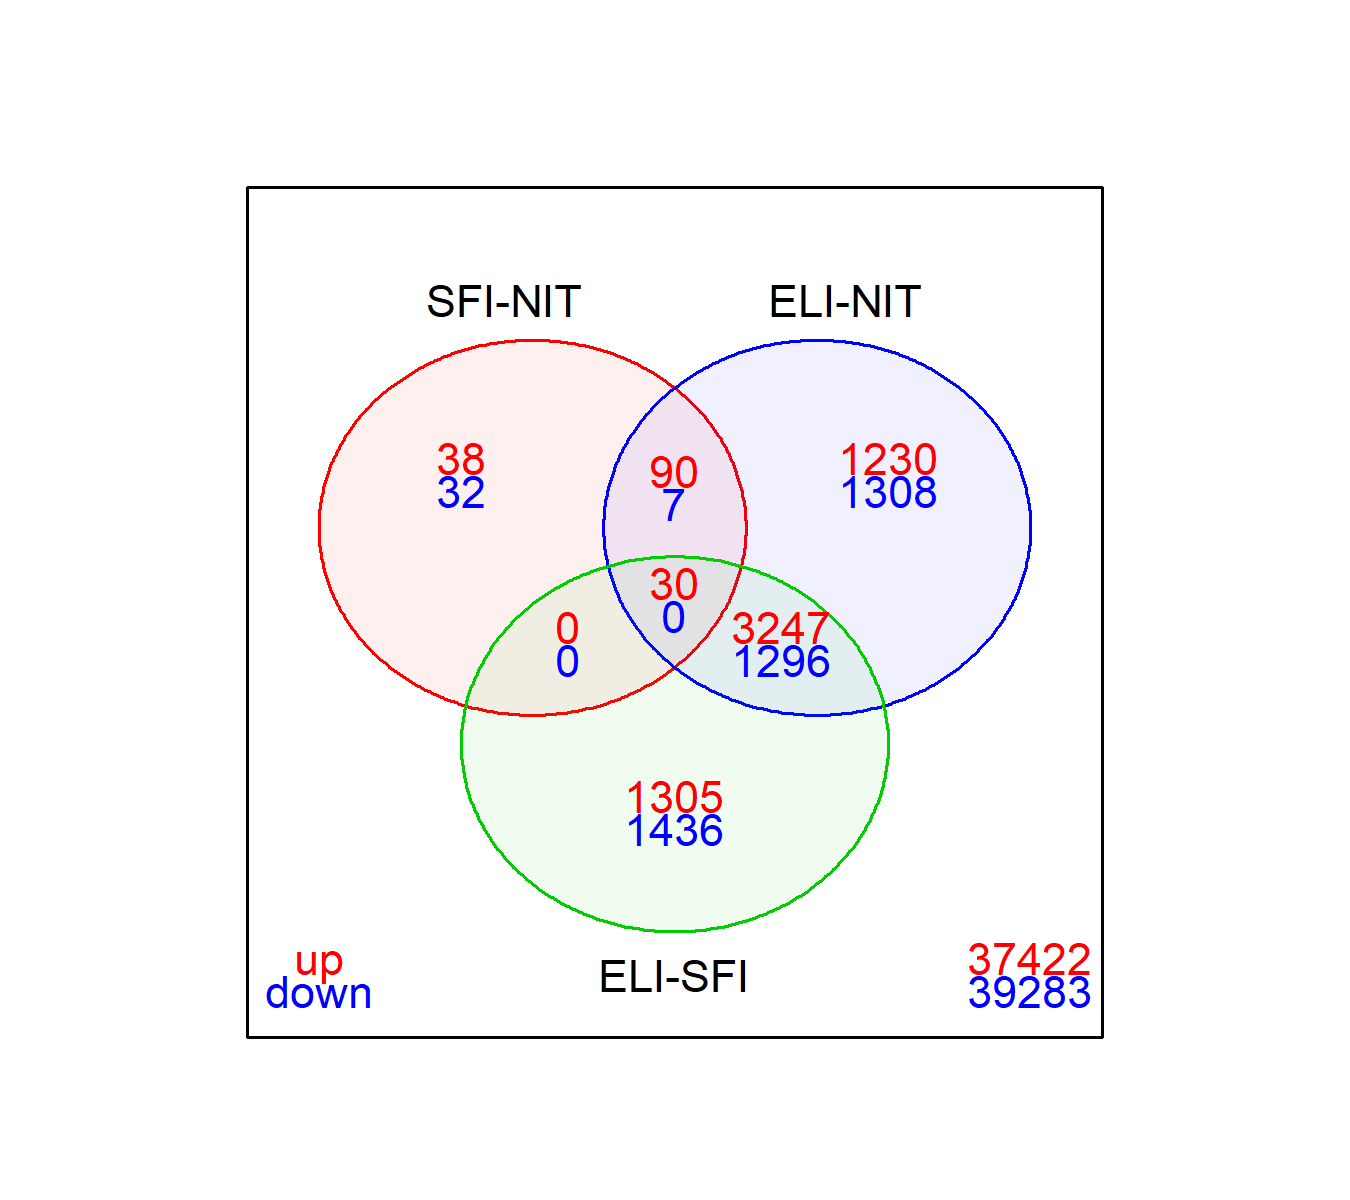
\includegraphics[width=0.8\linewidth]{results/5.CompComp/1.Venn} 

}

\caption{Diagrama de Venn que indica el número de tránscripts sobre-expresados (rojo) o infra-expresados (azul) en común entre los contrastes realizados. También se muestra aquellos tránscripts sin cambio de expresión significativa fuera de los círculos.}\label{fig:Fig13}
\end{figure}

Finalmente, hay 30 genes que se encuentran sobre-expresados en todas las
comparaciones, es decir, cuyo nivel de expresión es significativamente
mayor en ELI que en SFI y este es superior que en NIT. Este conjunto de
genes son aquellos cuya expresión incrementa significativamente con las
categorías y tamaño de infiltración. A partir de la comparación entre
las comparaciones se pueden definir conjuntos de tránscripts de interés.
Así pues, se puede estudiar con más detalle un grupo concreto, como
estos 30 genes sobre-expresados en cada nivel. Un gráfico de
\emph{counts} de 6 de los 30 tránscripts de este grupo confirma lo que
indica el diagrama de Venn, ya que se puede ver claramente que el nivel
de expresión de estos tránscripts incrementa con el tamaño de
infiltración (ELI\textgreater SFI\textgreater NIT) (Figura
\ref{fig:Fig14}). Identificar estos genes no hubiera sido posible sin
comparar las comparaciones entre ellas.

\begin{figure}

{\centering 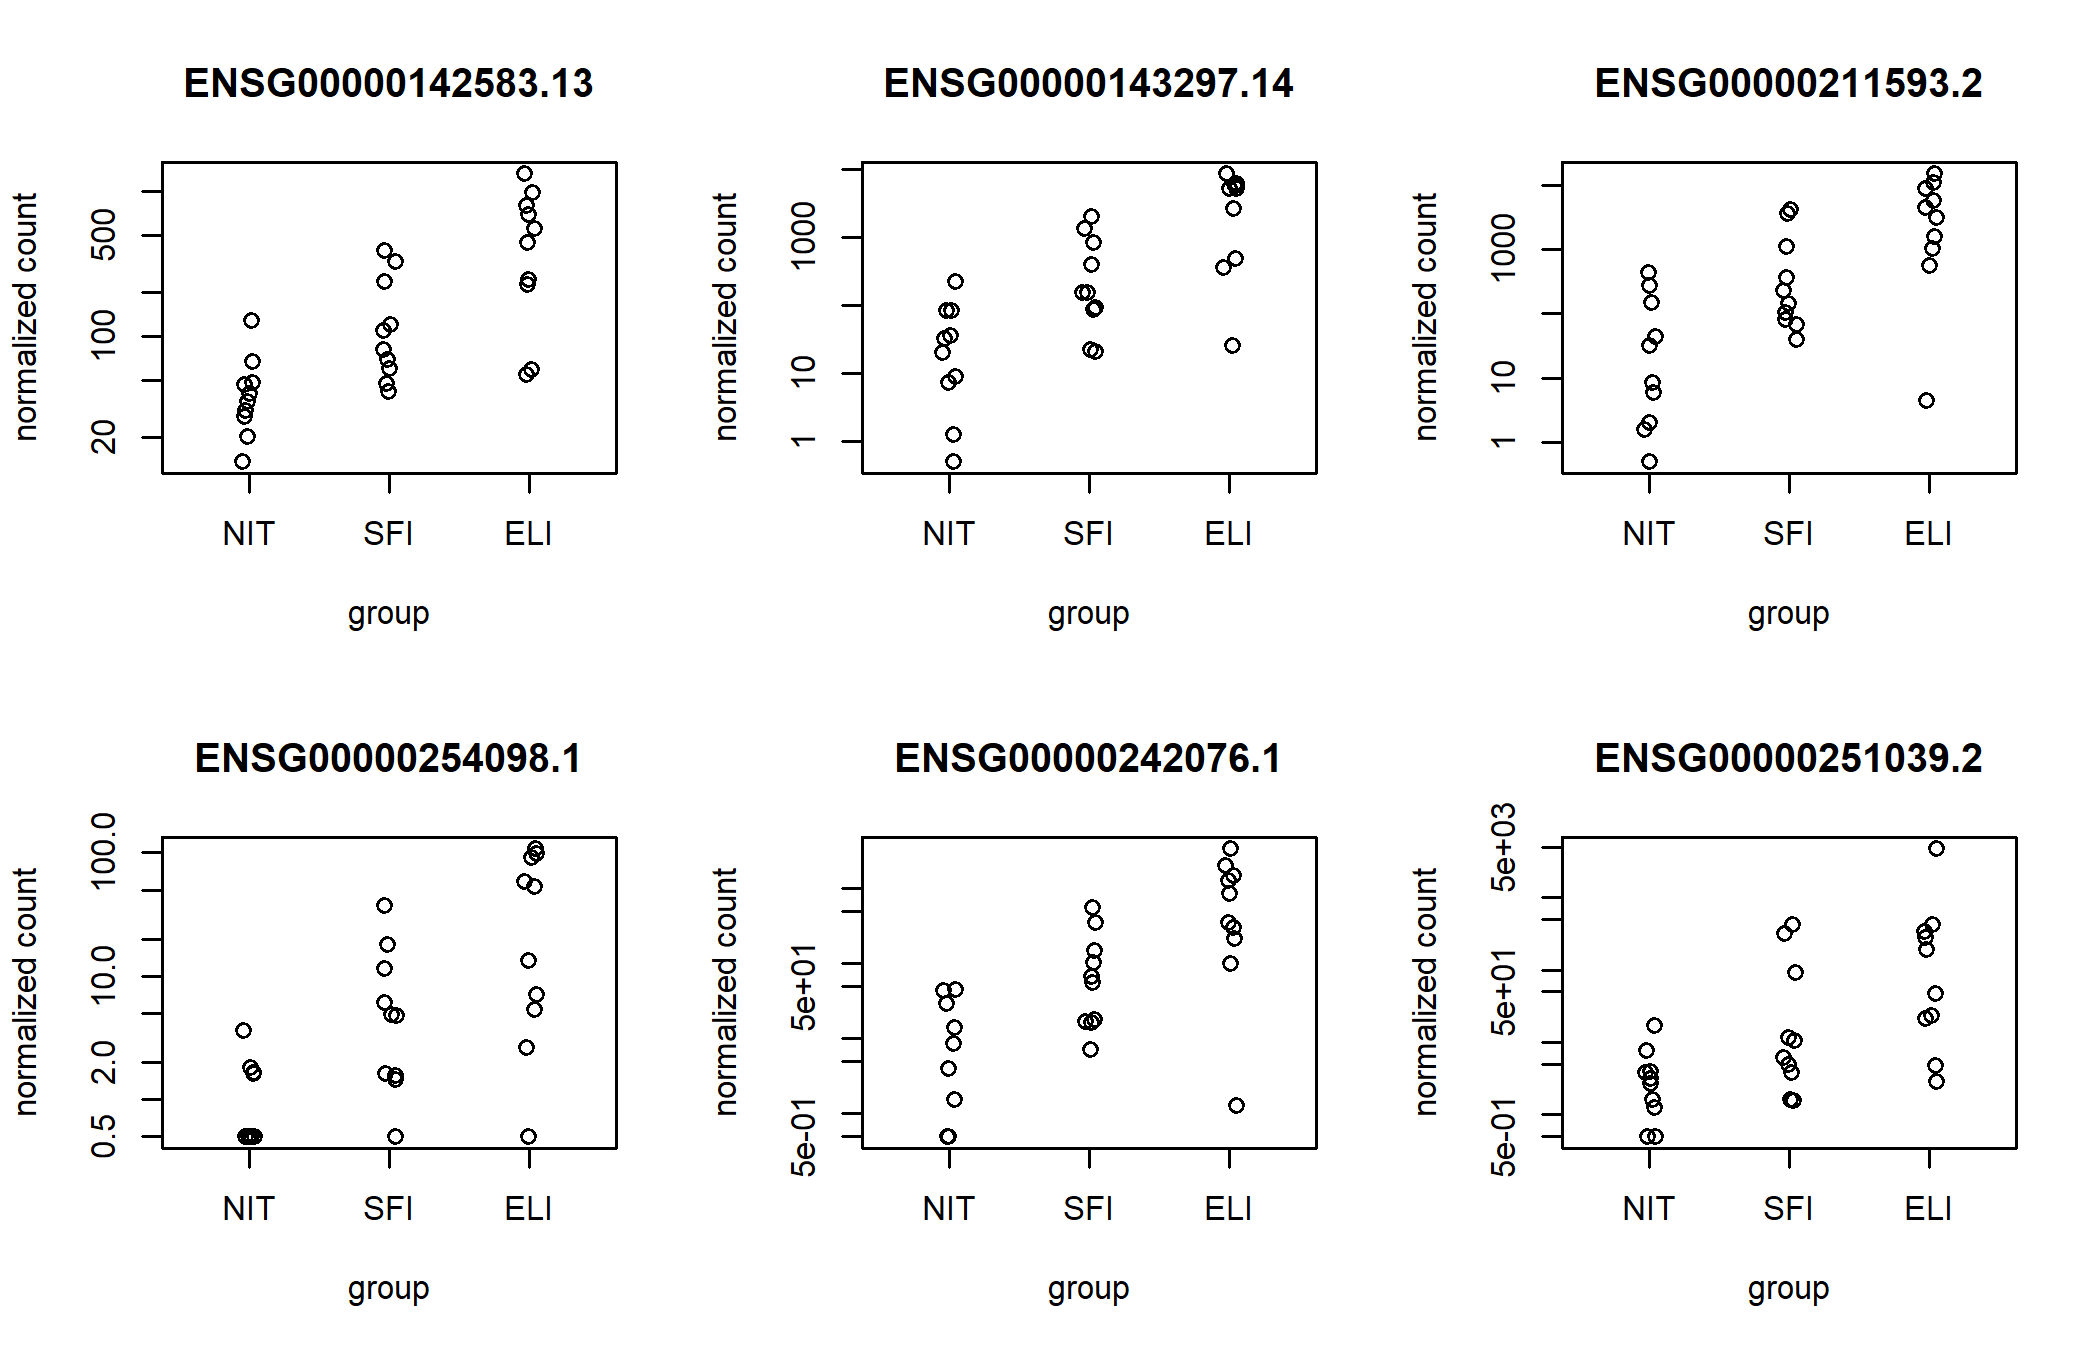
\includegraphics[width=0.8\linewidth]{results/5.CompComp/3.VennCts2} 

}

\caption{Cambio del número de counts de 6 de los 30 tránscripts cuya expresión cambia significativamente con cada tipo de infiltración, representados por cada muestra según el tipo de infiltración.}\label{fig:Fig14}
\end{figure}

Del mismo modo, puede estudiarse otro conjunto de tránscripts de
interés, como los 7 tránscripts infra-expresados en las comparaciones
SFI-NIT y ELI-NIT pero no en ELI-SFI. Estos tránscripts son los
tránscripts cuya expresión disminuye con la presencia de infiltraciones
cancerígenas, ya que su expresión cambia en los dos tipos de
infiltraciones al compararlos con las muestras no infiltradas (NIT). Los
gráficos de \emph{counts} para estos 7 tránscripts confirman que su
nivel de expresión es mayor en la muestra \texttt{NIT} que en las otras
dos muestras, y efectivamente el nivel de expresión es similar entre ELI
y SFI y no aparecen expresados diferencialmente en el contraste ELI-SFI
(Figura \ref{fig:Fig15}).

\begin{figure}

{\centering 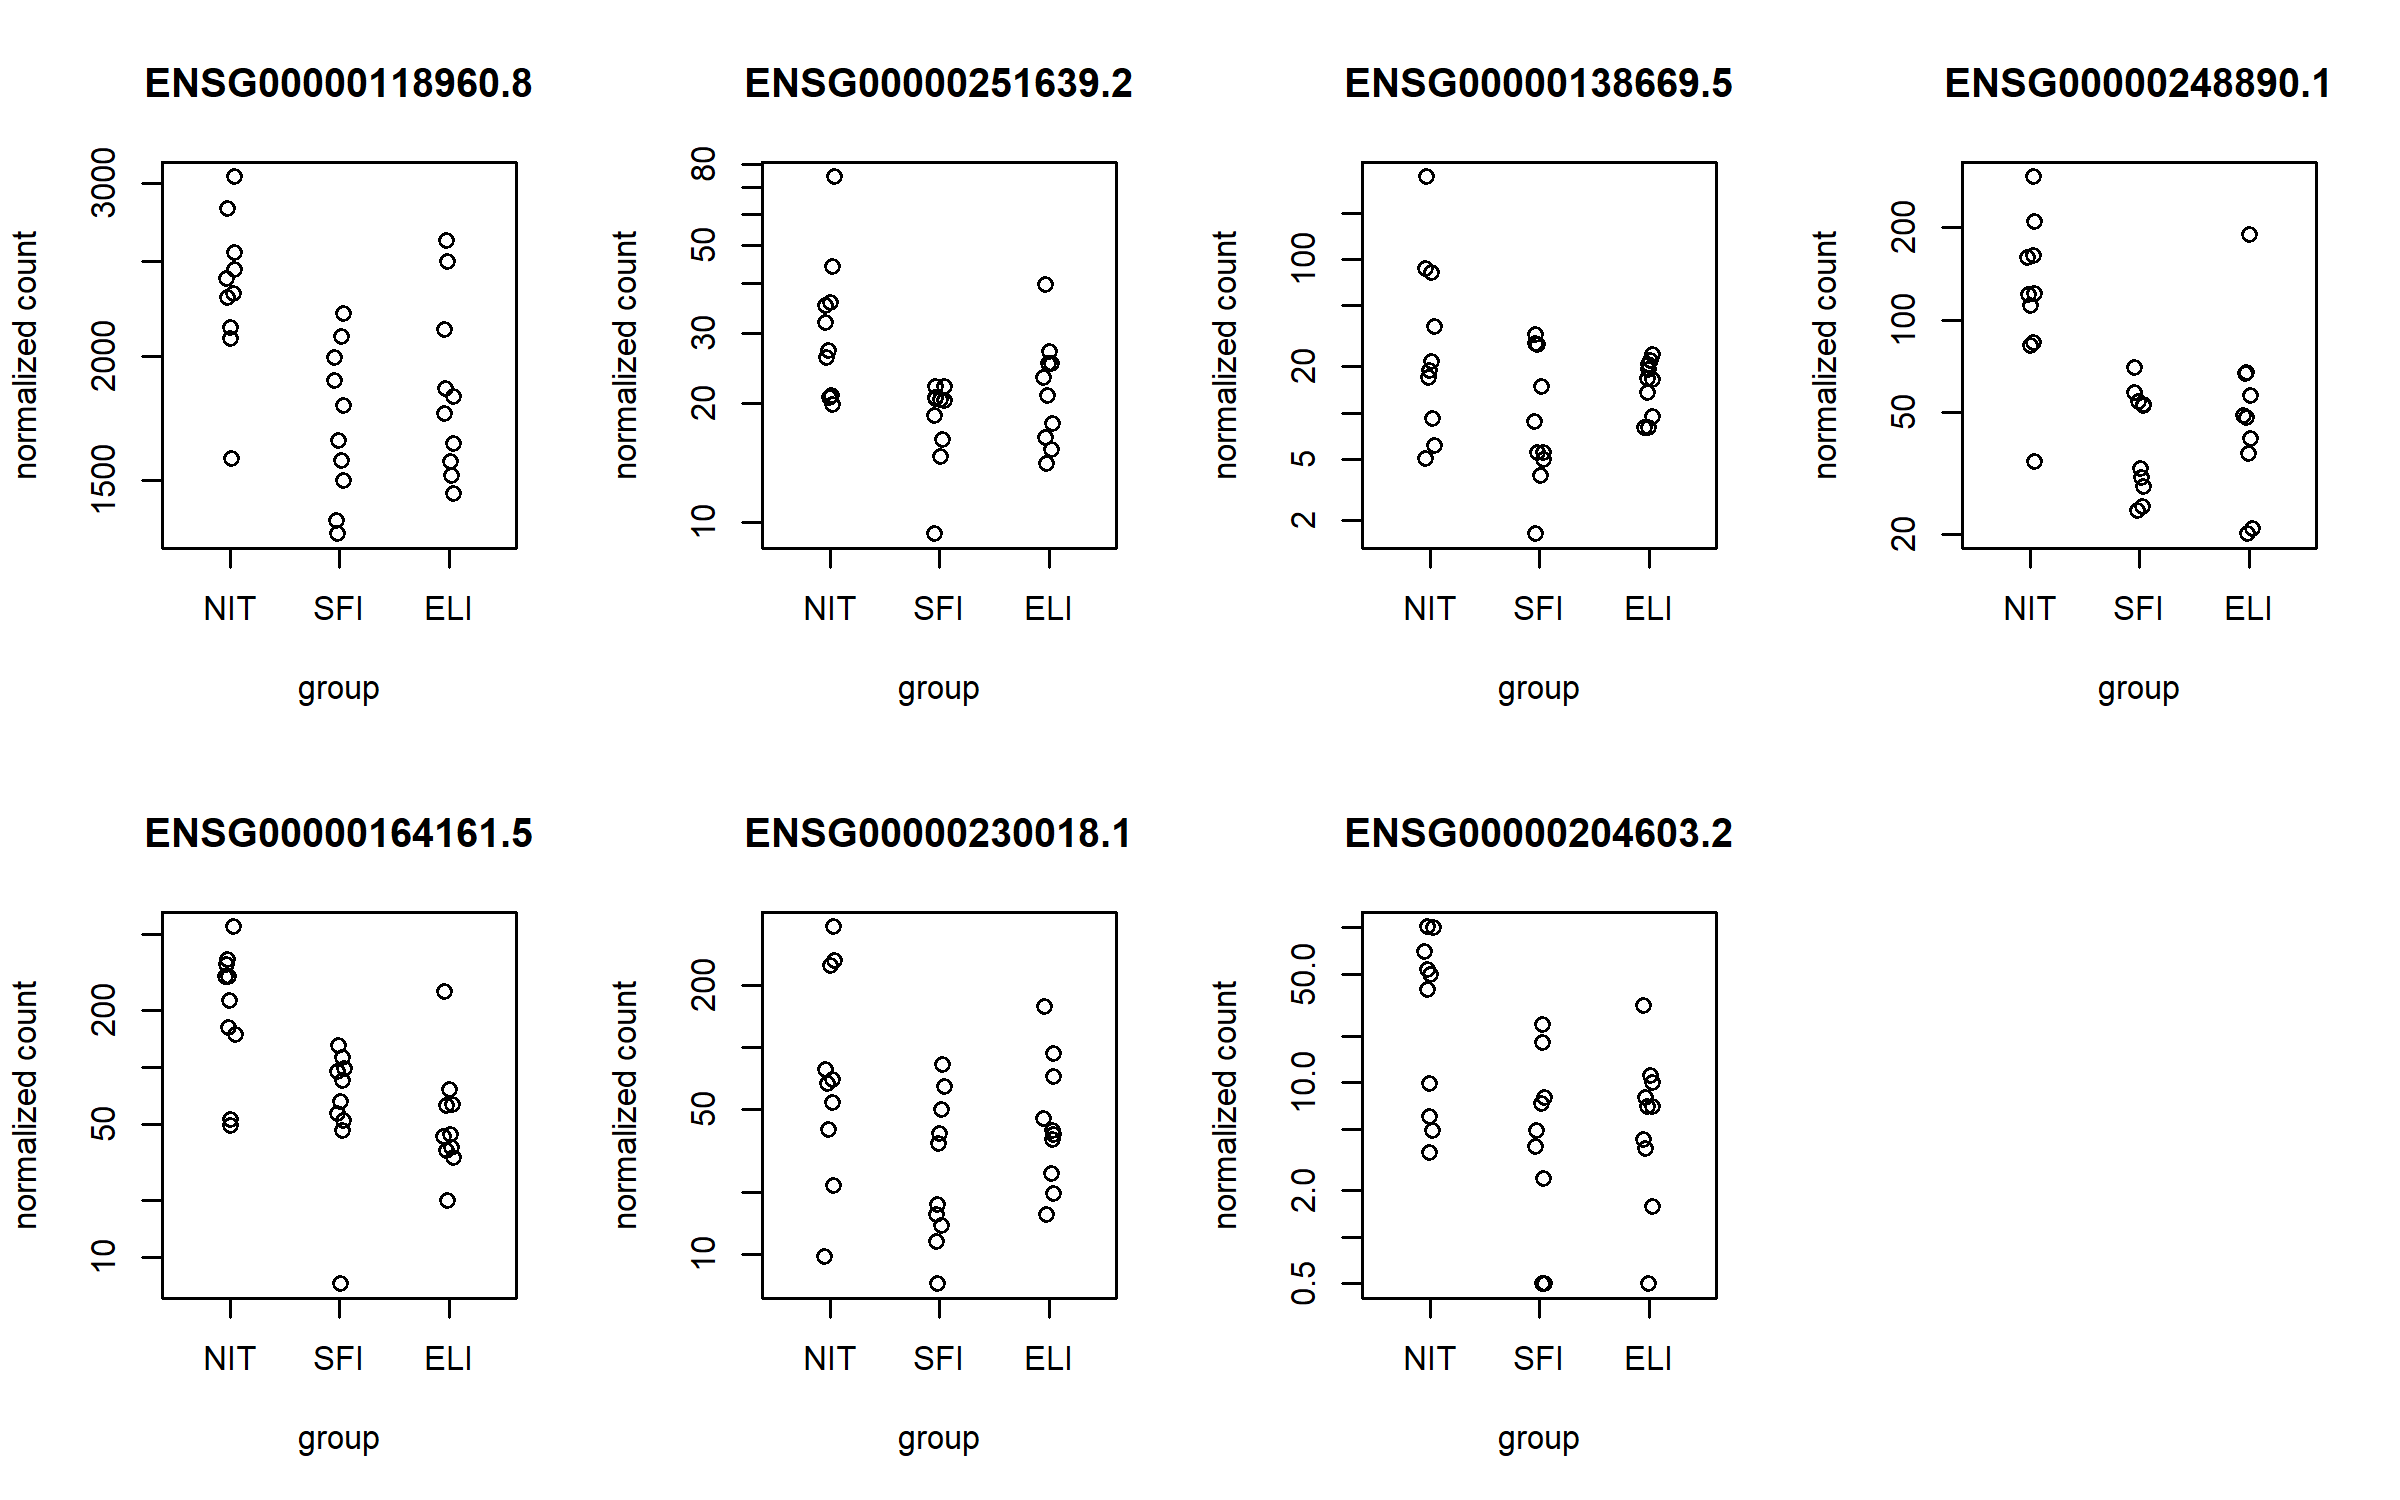
\includegraphics[width=0.8\linewidth]{results/5.CompComp/2.VennCts} 

}

\caption{Cambio del número de counts de los 7 tránscripts cuya expresión disminuye significativamente en la presencia de infiltraciones, representados por cada muestra según el tipo de infiltración.}\label{fig:Fig15}
\end{figure}

\hypertarget{anuxe1lisis-de-significaciuxf3n-bioluxf3gica-1}{%
\subsection{4.4. Análisis de significación
biológica}\label{anuxe1lisis-de-significaciuxf3n-bioluxf3gica-1}}

El objetivo inicial del estudio es identificar los mecanismos biologicos
afectados por el tamaño de la infiltración. Para conseguirlo resulta más
útil estudiar como cambian las funciones biológicas que el nivel de
tránscripts individuales. Así pues, a partir de las anotaciones de estos
tránscripts se puede estudiar el cambio de la representación de los
términos GO.

Previamente se ha mostrado los términos GO de los tránscripts con mayor
cambio de expresión (Tablas 3-8), pero esto no indica que la función
biológica que representan sea la función biológica que más ha variado.
Para obtener información de los cambios de funciones biológicas, además
de tener en cuenta el nivel del cambio de los tránscripts, se tiene en
cuenta el número de tránscripts con una función biologica similar cuya
expresión se ve afectada. Por ejemplo, el tránscript con mayor
\emph{Fold Change} podría estar relacionado con cierta función
\texttt{X} pero ser el único, mientras que muchos tránscripts de menor
efecto podrían estar relacionados con la función \texttt{Y}. En un caso
así, es probable que sea la función \texttt{Y} la más afectada por el
tipo de infiltración. Así pues, en esta sección se considera todo el
conjunto de genes significativos (\emph{p-valor} ajustado menor de 0.1,
log2FoldChange distinto de cero) para obtener información de las
funciones biológicas más afectadas por el tipo de infilitración, y no
solamente aquellos con mayor efecto.

Así pues, se obtiene una lista de los 6 términos GO (equivalentes a
funciones biologicas) más abundantes en el conjunto de genes
significativos de cada comparación (Tablas 9-11). De este modo, se
pueden deducir algunas de las funciones biologicas más afectadas por el
tipo de infiltración. Nótese que estas funciones se encuentran presentes
en cerca de un \(10\%\) de los genes con expresión significativa. El
nivel de los términos GO en este caso es muy detallado y se puede ver
que afectan a funciones biológicas básicas involucradas en la regulación
génica y mecanismos celulares.

\begin{table}

\caption{\label{tab:unnamed-chunk-4}Términos GO más abundantes entre los genes expresados diferencialmente entre SFI y NIT.}
\centering
\begin{tabular}[t]{lllr}
\toprule
  & Description & GeneRatio & p.adjust\\
\midrule
GO:0003713 & transcription coactivator activity & 4/60 & 0.0229320\\
GO:0008509 & anion transmembrane transporter activity & 4/60 & 0.0248351\\
GO:0140098 & catalytic activity, acting on RNA & 4/60 & 0.0417993\\
GO:0015179 & L-amino acid transmembrane transporter activity & 3/60 & 0.0008127\\
GO:0015171 & amino acid transmembrane transporter activity & 3/60 & 0.0020242\\
\addlinespace
GO:0015238 & drug transmembrane transporter activity & 3/60 & 0.0037560\\
\bottomrule
\end{tabular}
\end{table}

\begin{table}

\caption{\label{tab:unnamed-chunk-5}Términos GO más abundantes entre los genes expresados diferencialmente entre ELI y NIT.}
\centering
\begin{tabular}[t]{lllr}
\toprule
  & Description & GeneRatio & p.adjust\\
\midrule
GO:0050839 & cell adhesion molecule binding & 156/4391 & 0.0005615\\
GO:0005543 & phospholipid binding & 151/4391 & 0.0000006\\
GO:0031267 & small GTPase binding & 139/4391 & 0.0009256\\
GO:0017016 & Ras GTPase binding & 136/4391 & 0.0006617\\
GO:0016887 & ATPase activity & 125/4391 & 0.0003386\\
\addlinespace
GO:0003779 & actin binding & 123/4391 & 0.0409742\\
\bottomrule
\end{tabular}
\end{table}

\begin{table}

\caption{\label{tab:unnamed-chunk-6}Términos GO más abundantes entre los genes expresados diferencialmente entre ELI y SFI.}
\centering
\begin{tabular}[t]{lllr}
\toprule
  & Description & GeneRatio & p.adjust\\
\midrule
GO:0050839 & cell adhesion molecule binding & 165/4543 & 0.0001109\\
GO:0031267 & small GTPase binding & 154/4543 & 0.0000106\\
GO:0017016 & Ras GTPase binding & 149/4543 & 0.0000154\\
GO:0005543 & phospholipid binding & 148/4543 & 0.0000185\\
GO:0004674 & protein serine/threonine kinase activity & 136/4543 & 0.0065302\\
\addlinespace
GO:0004175 & endopeptidase activity & 130/4543 & 0.0139414\\
\bottomrule
\end{tabular}
\end{table}

Los mismos resultados se pueden representar visualmente utilizando las
funciones de la liberería \texttt{clusterProfiler}. En la representación
con puntos de los 30 términos GO más enriquecidos en la comparación
ELI-SFI (Figura \ref{fig:Fig16}) puede verse que los primeros
corresponden a los mostrados en la tabla (Tabla 11). En la
representación gráfica se puede ver la abundancia relativa de las
actividades en el eje vertical, con lo que se puede ver que las 10
primeras actividades tienen un valor de abundancia superior que el
resto, así proporcionando una idea de la función biológica afectada en
esta comparación. Por ejemplo, se ve que muchas de las actividades están
relacionadas con la actividad GTPasa.

\begin{figure}

{\centering 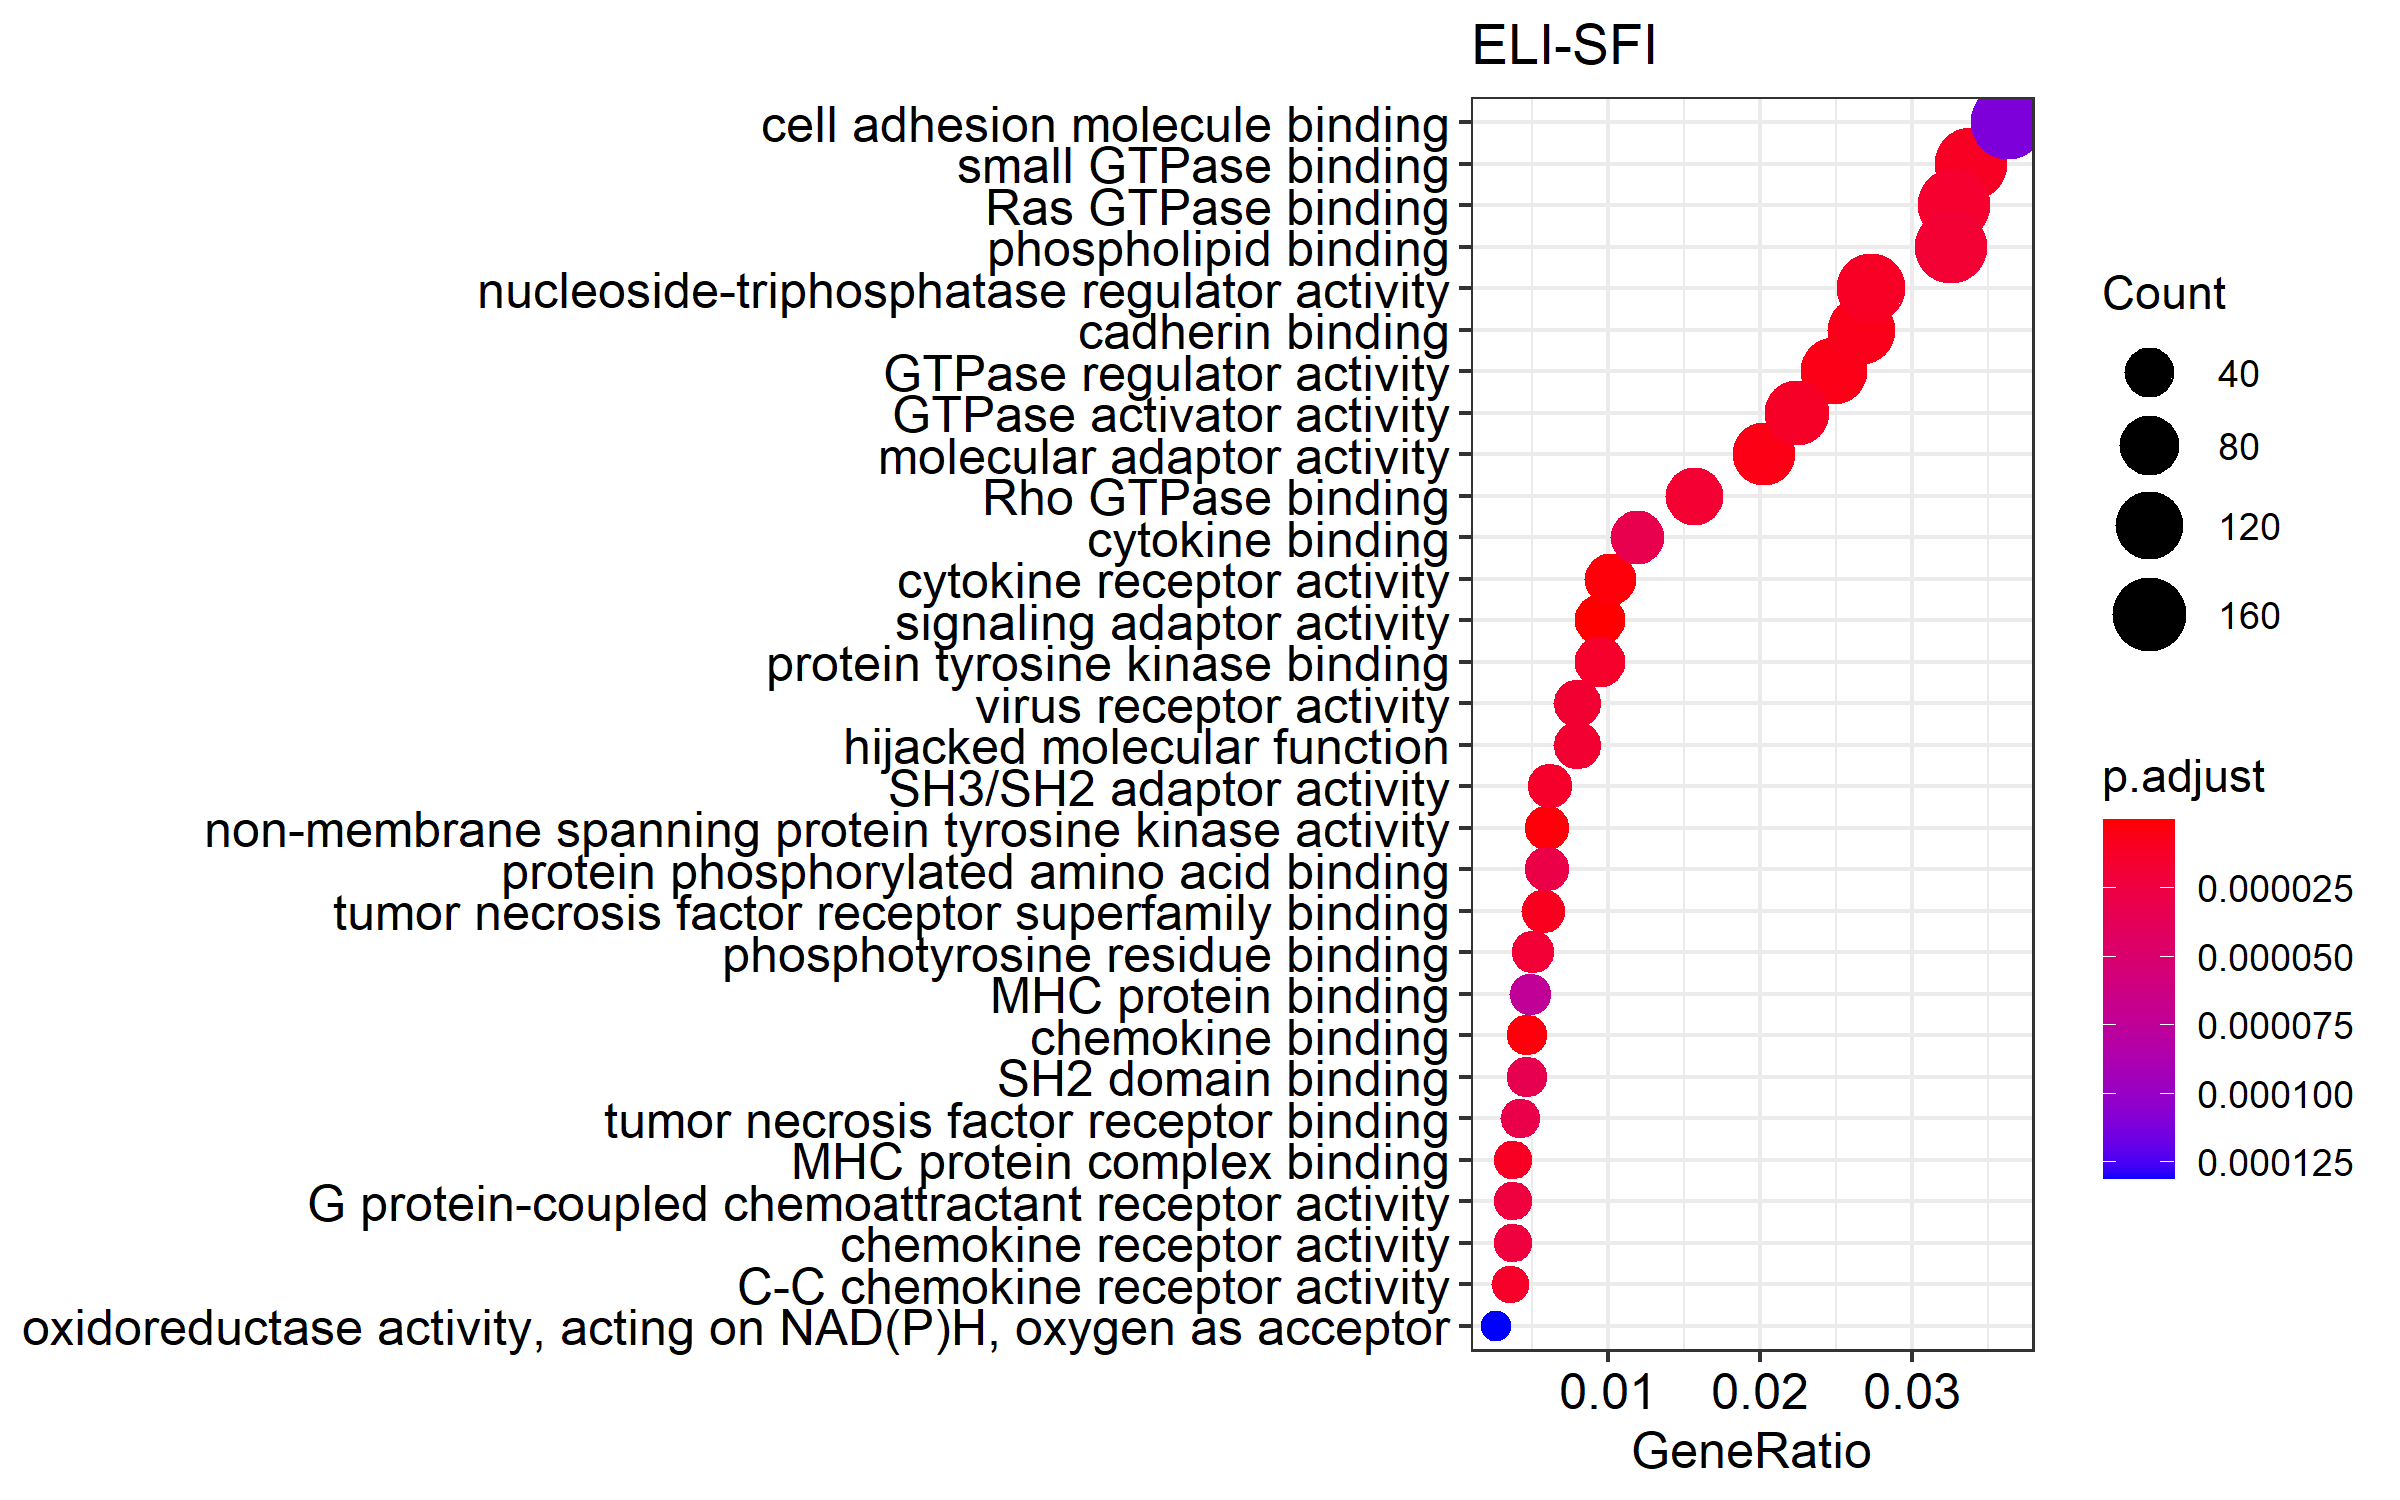
\includegraphics[width=0.8\linewidth]{results/6.GOterms/1.GOdots} 

}

\caption{Términos GO más abundantes entre los genes expresados diferencialmente entre ELI y SFI según su abundáncia y p-valor del enriquecimiento.}\label{fig:Fig16}
\end{figure}

Quizás una forma más interesante de interpretar estas relaciones es a
través de la formación de redes que muestran la similitud entre diversos
términos GO enriquecidos en una comparación, como se muestra a
continuación para la comparación SFI-NIT (Figura \ref{fig:Fig17}). Esta
figura indica que los términos GO afectados por la presencia de
infiltraciones SFI al compararla con muestras sin infiltración (NIT) se
podrían agrupar en grupos de actividad similar. El grupo con mayor
número de términos GO tiene que ver con cambios en los transportadores
de componentes metabolicos, indicando un posible cambio de metabolismo
con la aparición de infiltraciónes SFI. Otro grupo prevalente tiene que
ver con la actividad de unión de RNA polimerasa, indicando cambios en la
expresión génica entre las dos muestras. Es interesante ver que se
incluye el término GO con relación a unión a p53, que es un marcador
cancerígeno, puesto que se compara una muestra cancerígena (SFI) con una
que no lo es (NIT).

\begin{figure}

{\centering 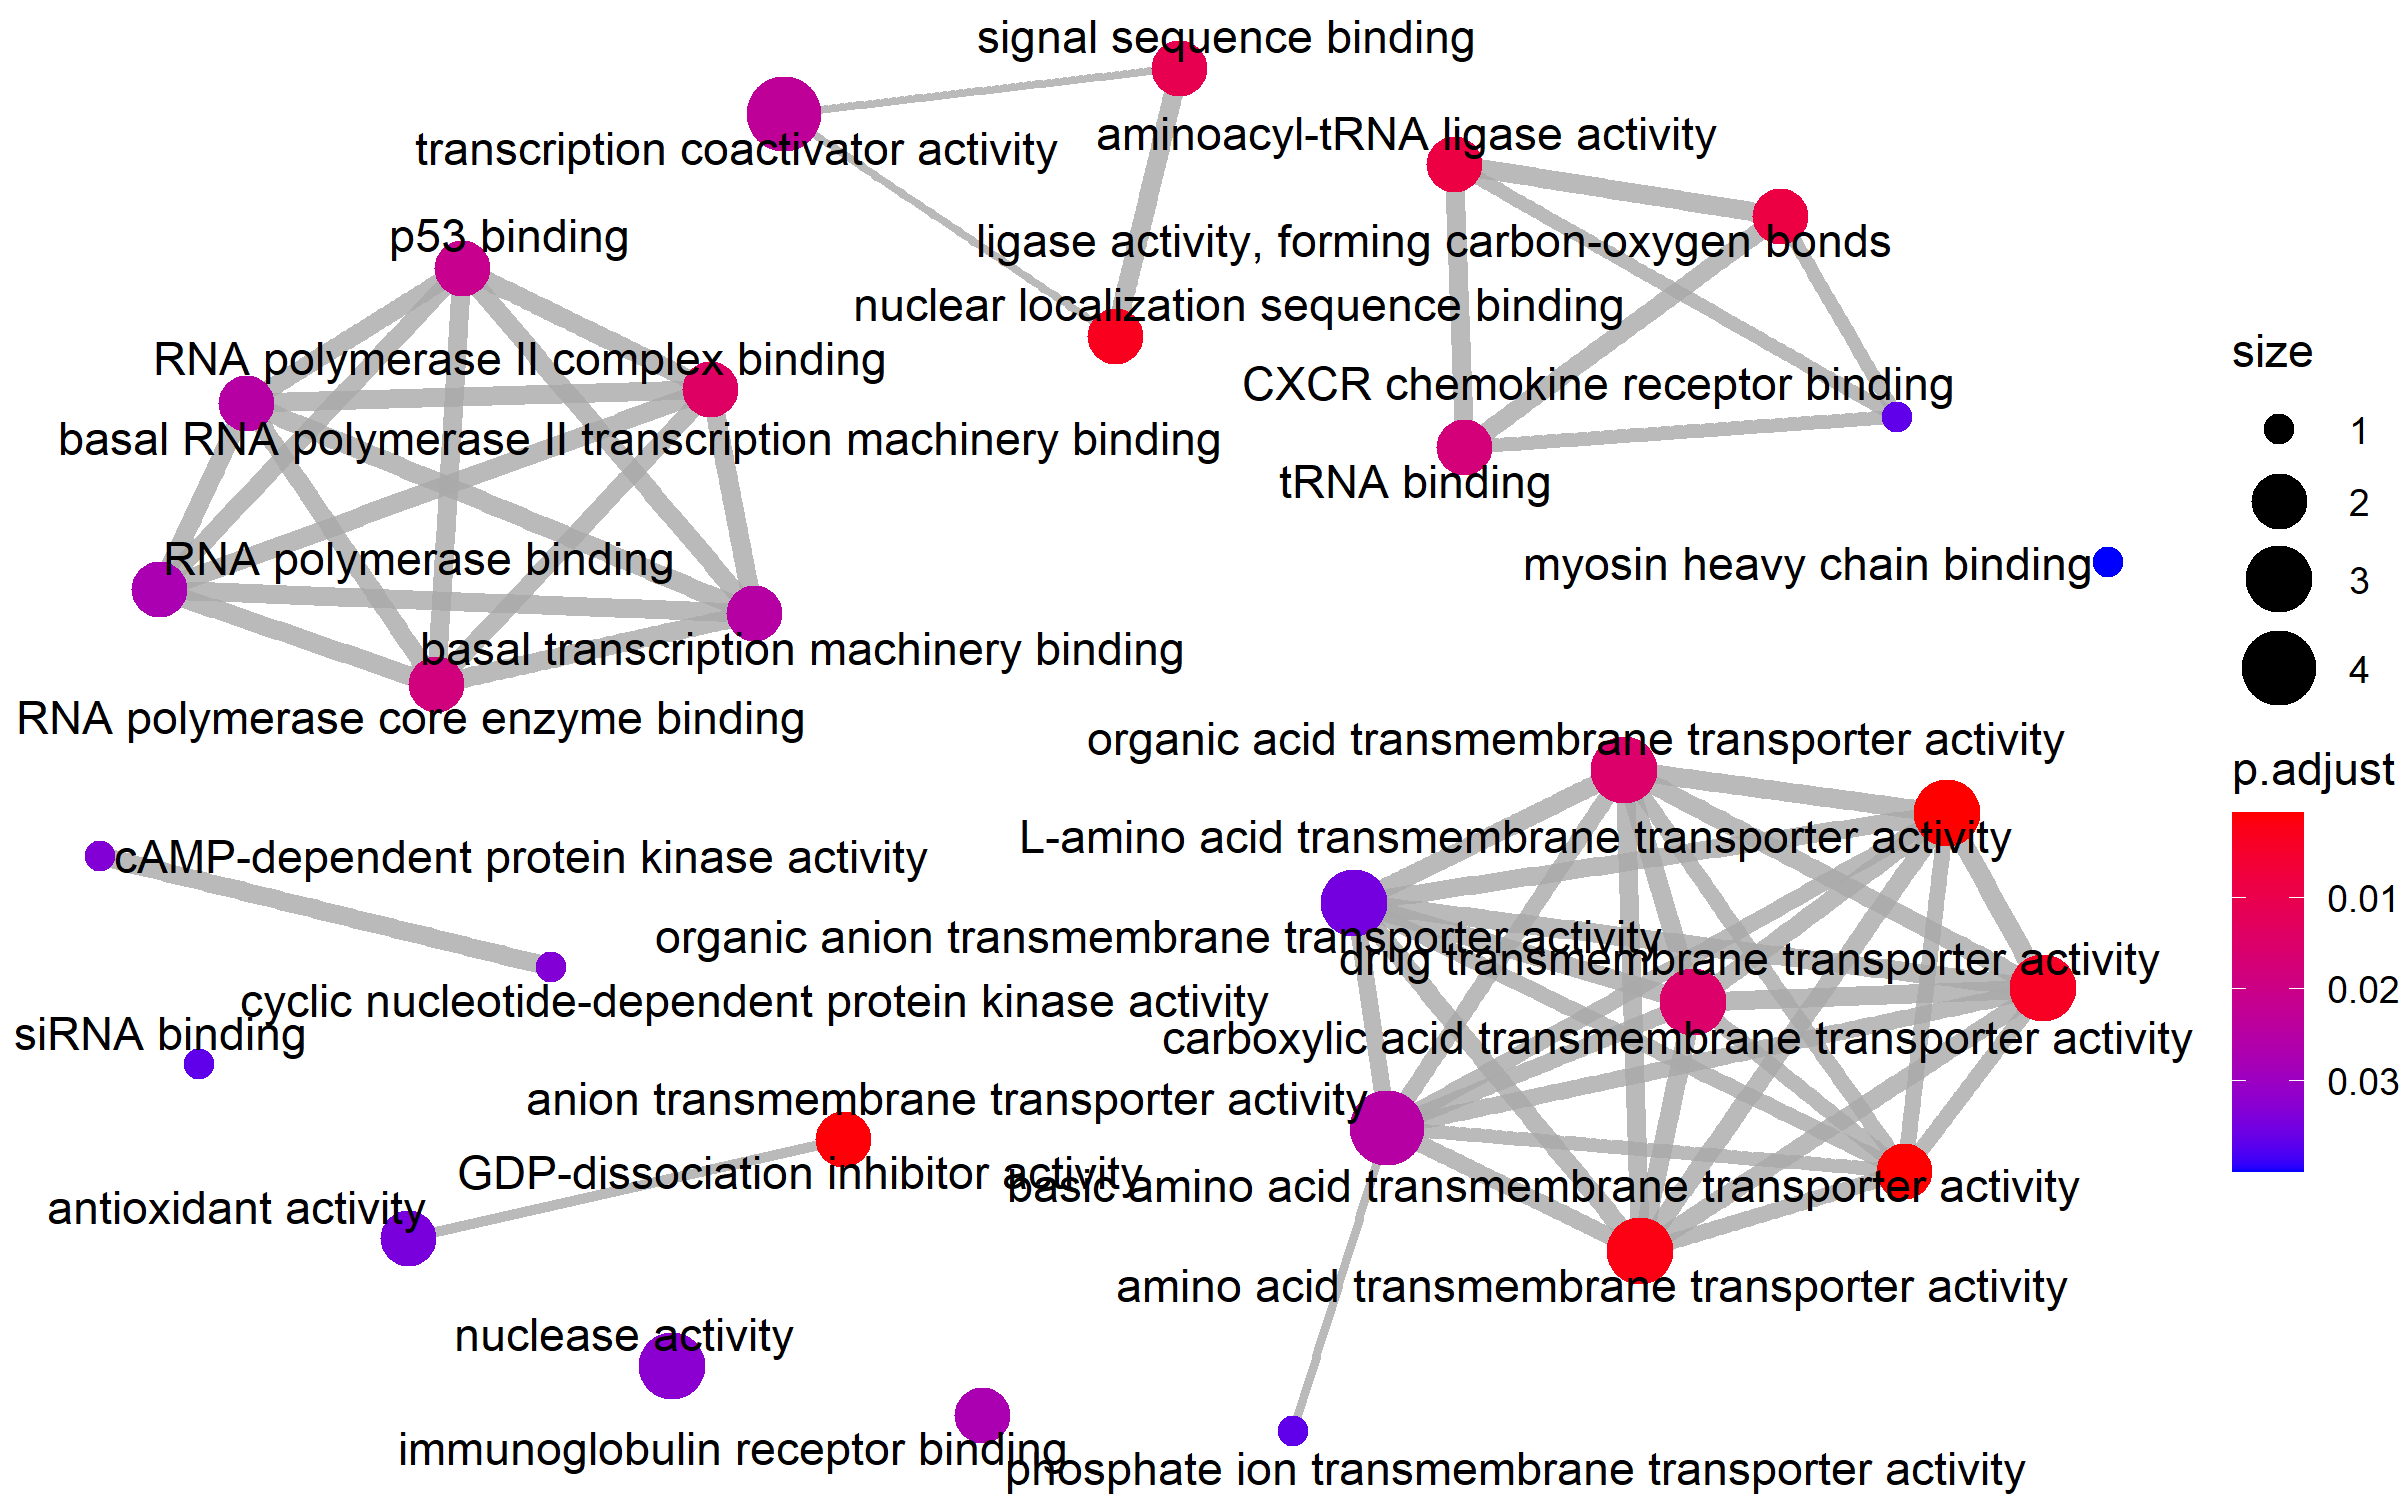
\includegraphics[width=0.8\linewidth]{results/6.GOterms/2.GOnet} 

}

\caption{Términos GO más abundantes entre los genes expresados diferencialmente entre SFI y NIT, agrupados en redes según su similitud de actividad biológica.}\label{fig:Fig17}
\end{figure}

Los términos GO se clasifican a varios niveles. Una clasificación
general es si indican un \emph{Biological Process} (BP), una
\emph{Molecular Function} (MF), o el \emph{Cellular Component} (CC) con
el que están involucrados. Así mismo, hay distintos niveles de detalle.
Utilizando estos para filtrar los términos GO de interés, se puede ver
que la mayoría de términos GO enriquecidos en el contraste ELI-SFI
tienen que ver con cambios metabólicos a distintos niveles (Tabla 12).

\begin{table}

\caption{\label{tab:unnamed-chunk-7}Términos GO de nivel 2 de Biological Process en la comparación entre ELI y SFI.}
\centering
\begin{tabular}[t]{llr}
\toprule
  & Description & Count\\
\midrule
GO:0050789 & regulation of biological process & 3109\\
GO:0071704 & organic substance metabolic process & 2942\\
GO:0050794 & regulation of cellular process & 2936\\
GO:0044237 & cellular metabolic process & 2874\\
GO:0044238 & primary metabolic process & 2840\\
\addlinespace
GO:0006807 & nitrogen compound metabolic process & 2724\\
\bottomrule
\end{tabular}
\end{table}

En los análisis anteriores solamente se tenía en cuenta la abundancia de
los términos GO, pero no la magnitud ni sentido (sobre- o infra-
expresión) de su efecto. Esta información se puede incorporar al
análisis de significación biologica realizando el \emph{Gene Enrichment
Analysis} (GEA). Para simplificar los resultados, se muestran solamente
los resultados para la comparación ELI-SFI en adelante. Los resultados
del GEA permiten representar las actividades biologicas afectadas en la
comparación ELI-SFI según si han sido activadas o suprimidas (Figura
\ref{fig:Fig18}). El resultado indica que procesos metabólicos
relacionados con el ciclo de Krebs son inhibidos mientras que se activa
el sistema immune con la aparición de infiltraciones.

\begin{figure}

{\centering 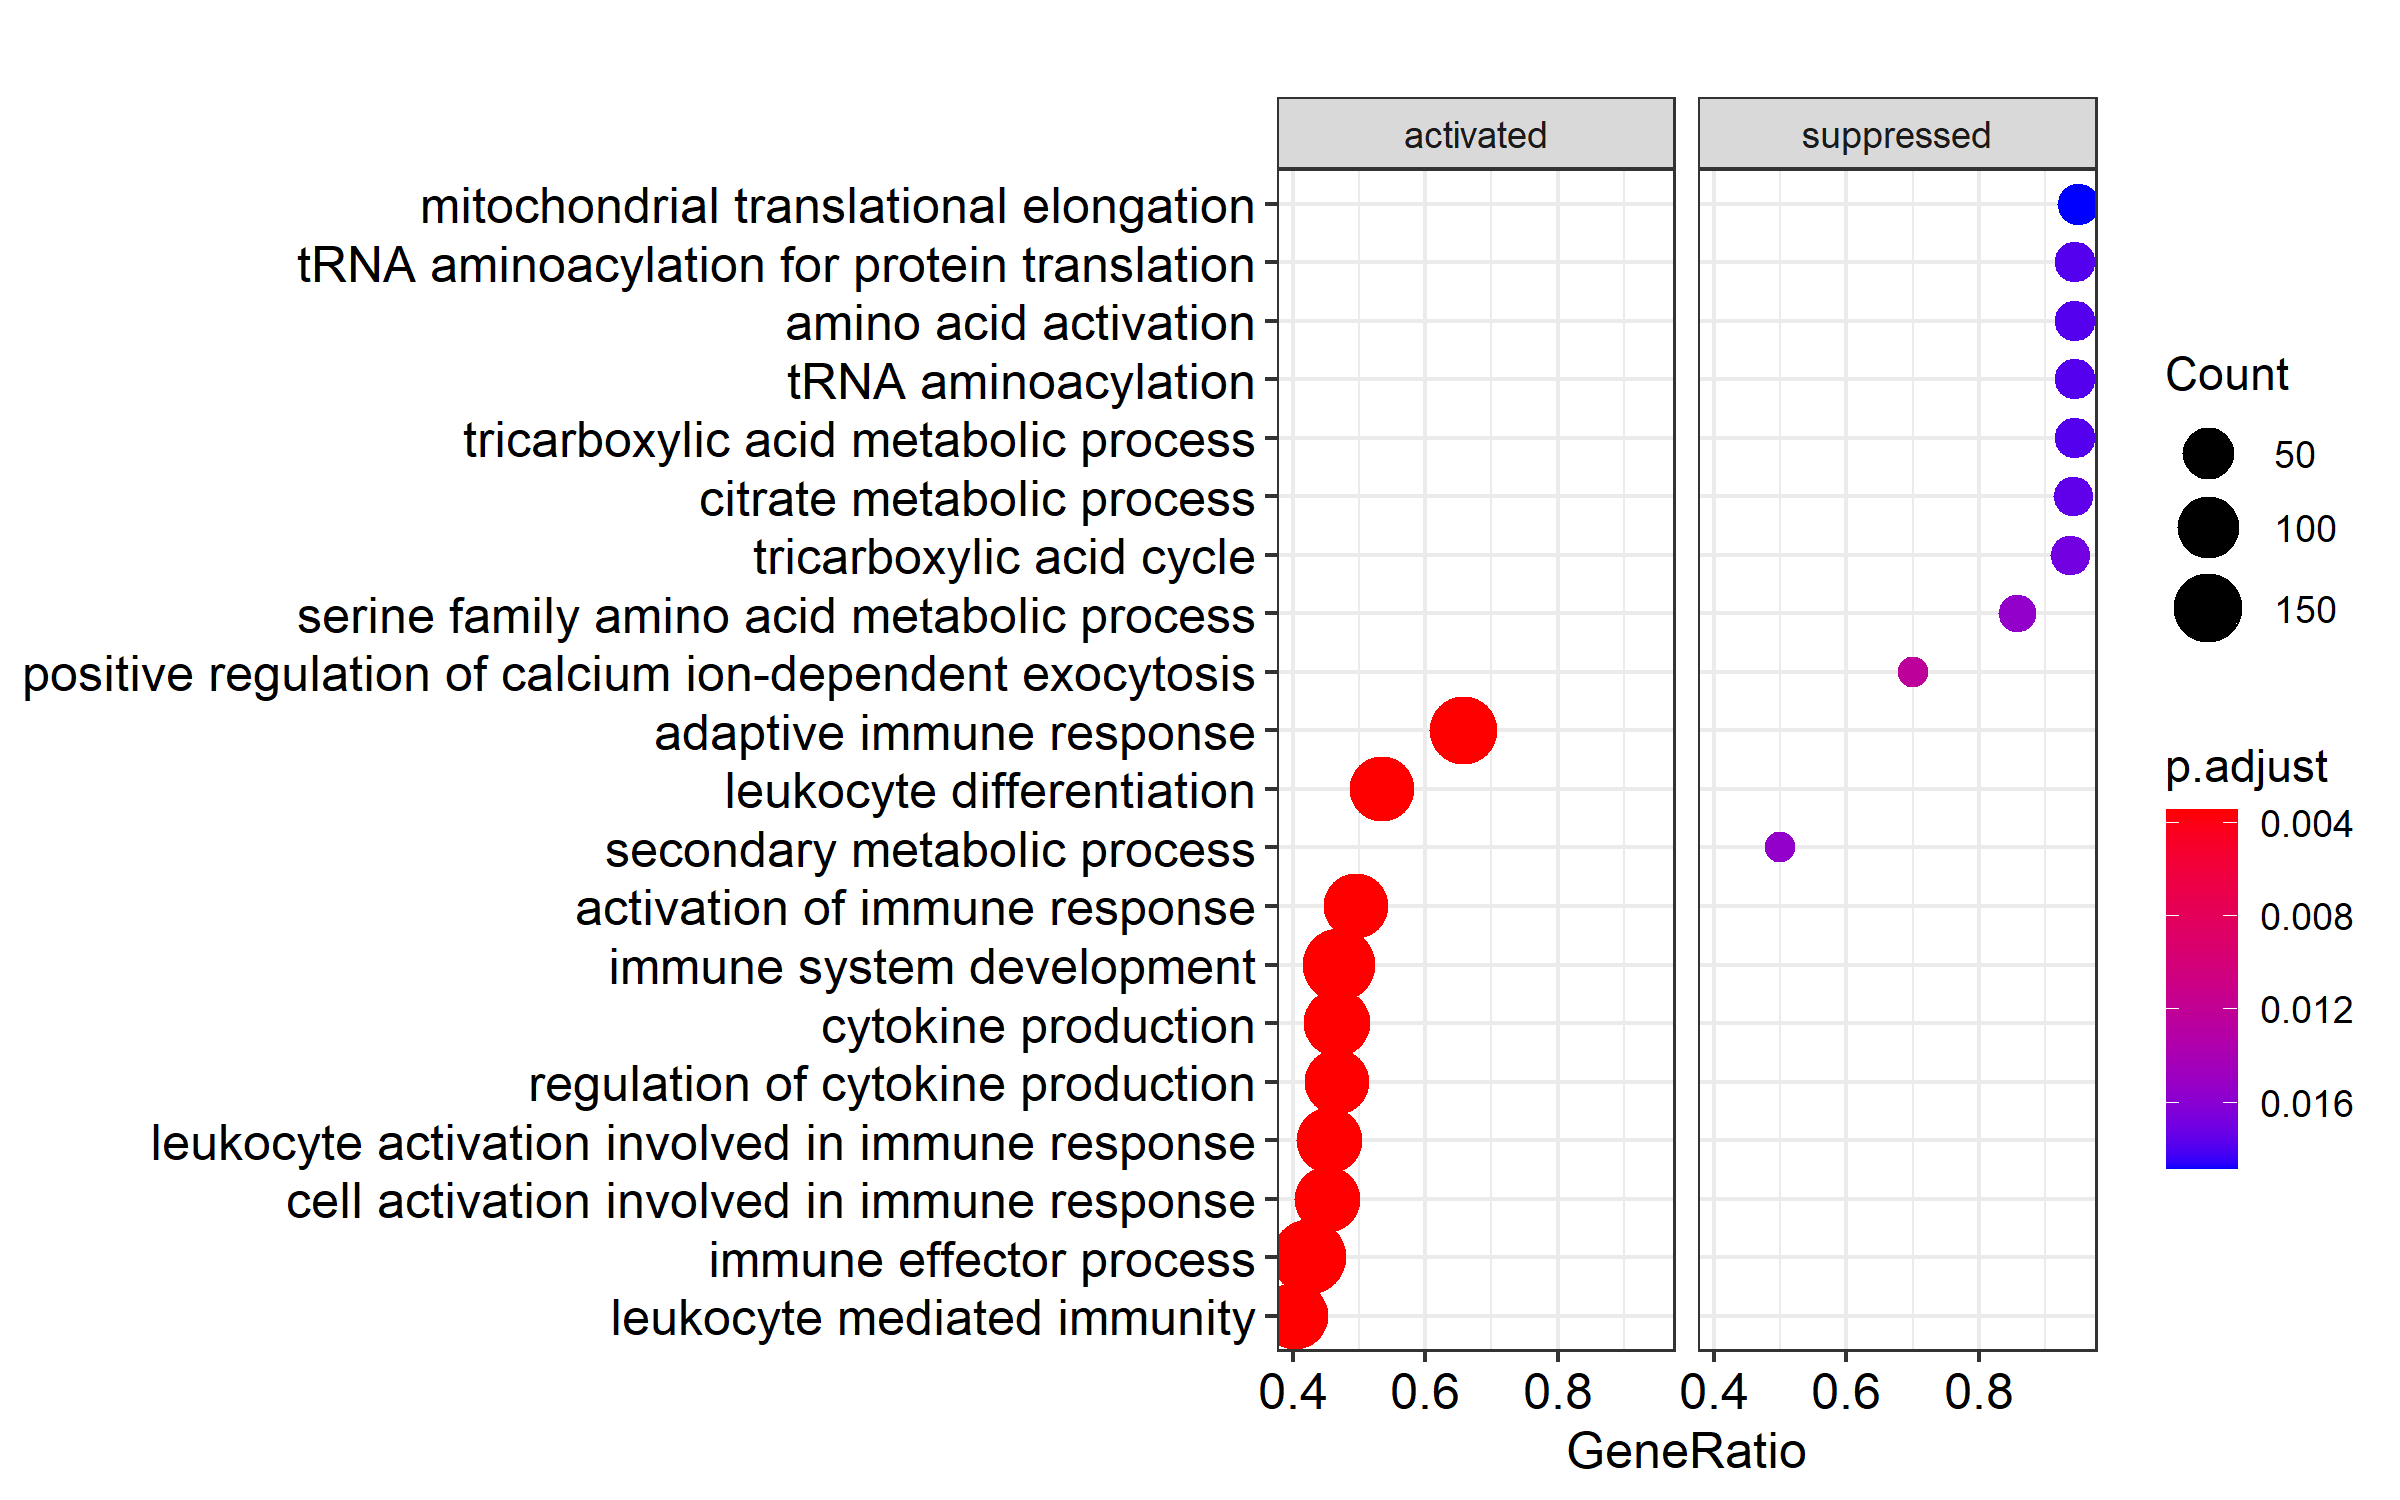
\includegraphics[width=0.8\linewidth]{results/6.GOterms/3.GOupDwn} 

}

\caption{Primeros 30 términos GO más enriquecidos en el contraste ELI-SFI según el efecto.}\label{fig:Fig18}
\end{figure}

Incluso es posible obtener información sobre los tejidos afectados por
el cambio de expresión. En este caso se observan solamente de
\texttt{lymphoma}, lo que encaja con que la comparación entre ELI-SFI
refleja cambios en la infiltración del limfoma y por lo tanto los genes
afectados tienen que ver con el limfoma (Figura \ref{fig:Fig19}).

\begin{figure}

{\centering 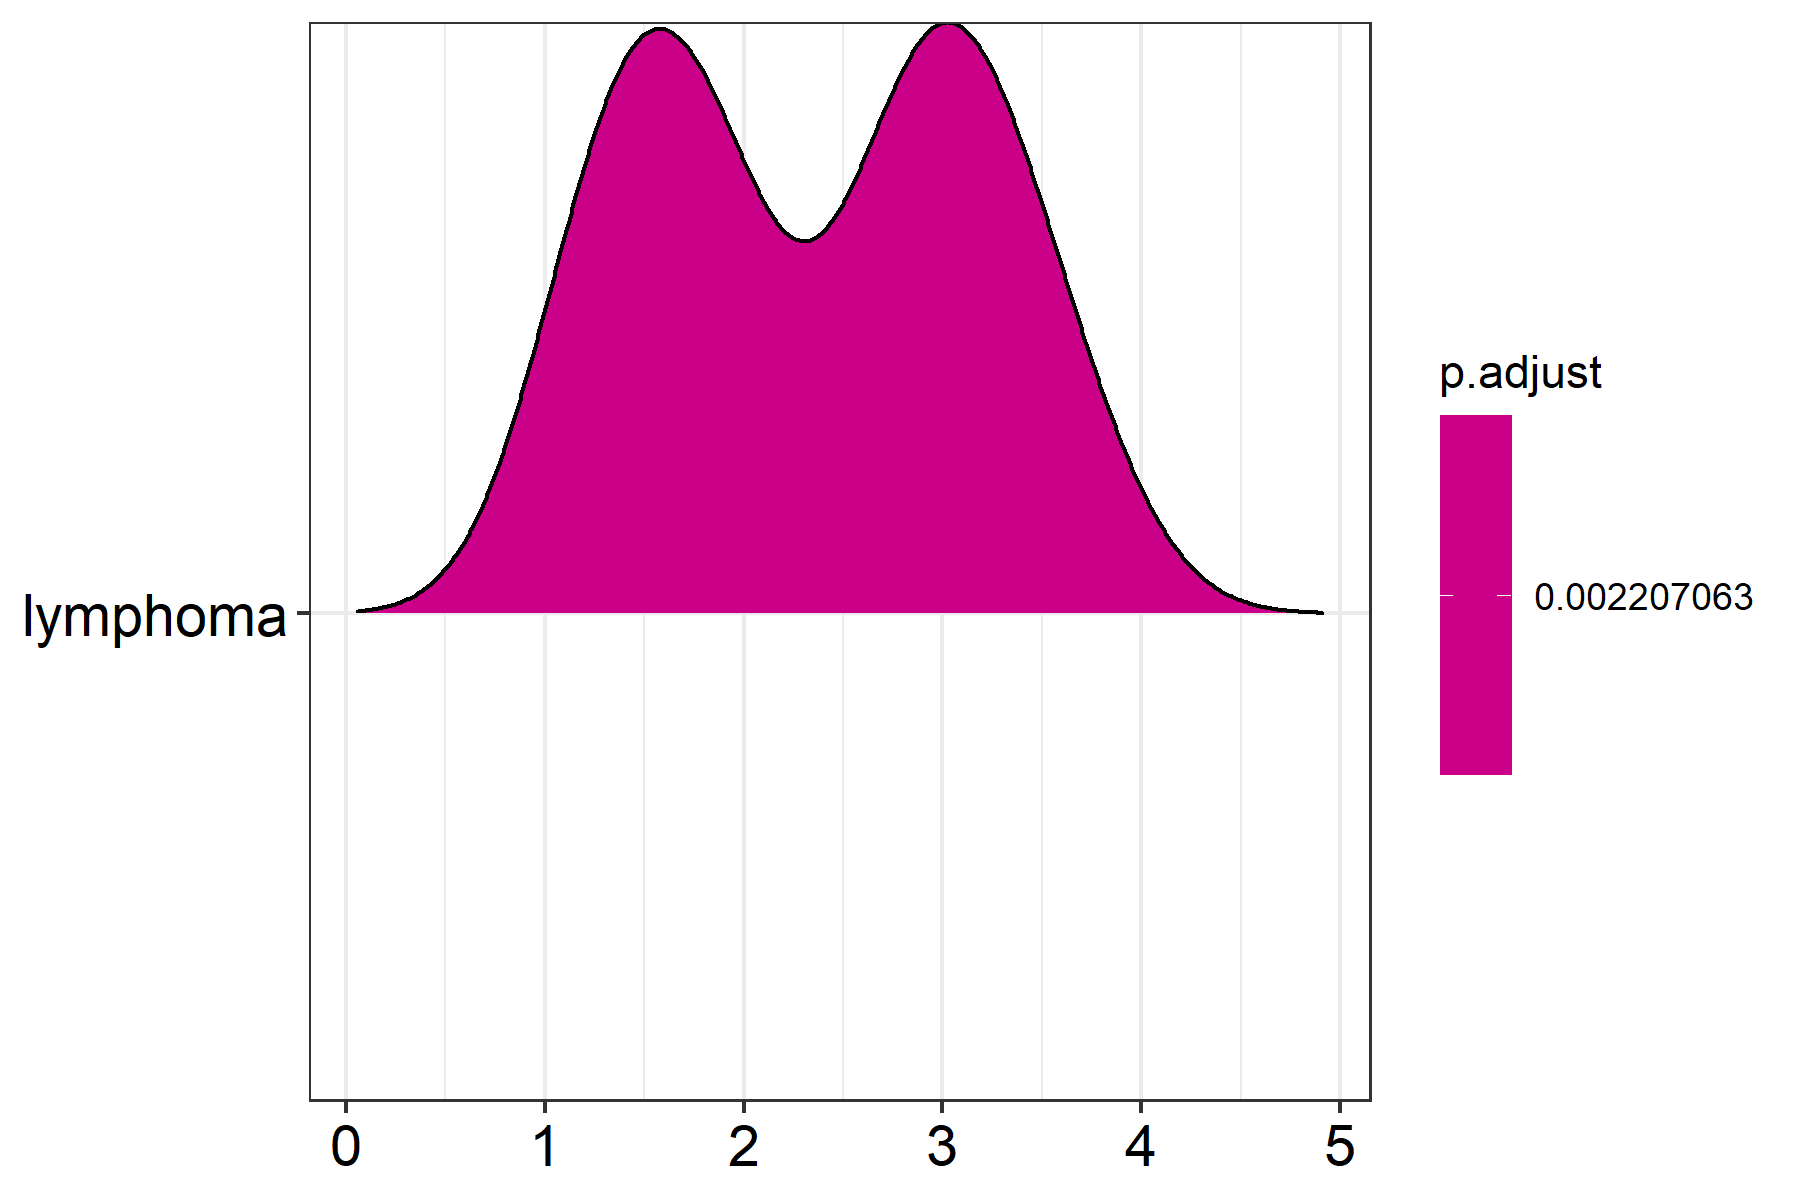
\includegraphics[width=0.8\linewidth]{results/6.GOterms/4.GOtiss} 

}

\caption{Distribución de los términos GO afectados significativamente en el contraste ELI-SFI según el tejido que afectan.}\label{fig:Fig19}
\end{figure}

Finalmente, tiniendo en cuenta el efecto de cada tránscript, puede
visualizarse con detalle las redes biologicas más afectadas al comparar
las muestras. Combinando la información de la base de redes biologicas
KEGG es posible ver las redes más afectadas por el cambio del tipo de
infiltración. Comparando ELI-SFI (Tabla 13) se puede ver que las vías
afectadas tienen relación con las el sistema immune.

\begin{table}

\caption{\label{tab:unnamed-chunk-8}Redes biológicas de KEGG más afectadas el comparar las muestrasa ELI y SFI. Se incluye el KEGG ID y nombre completo de cada red, junto con la magnitud de su enriquecimiento.}
\centering
\begin{tabular}[t]{llrr}
\toprule
  & Description & setSize & enrichmentScore\\
\midrule
hsa04060 & Cytokine-cytokine receptor interaction & 96 & 0.5955451\\
hsa04062 & Chemokine signaling pathway & 70 & 0.6122853\\
hsa04650 & Natural killer cell mediated cytotoxicity & 59 & 0.6241345\\
hsa04640 & Hematopoietic cell lineage & 54 & 0.6599108\\
hsa04660 & T cell receptor signaling pathway & 49 & 0.6823465\\
\addlinespace
hsa04061 & Viral protein interaction with cytokine and cytokine receptor & 39 & 0.6618534\\
\bottomrule
\end{tabular}
\end{table}

A partir de la información de las vias biológicas afectadas, se elige
visualizar con más detalle la vía \emph{Natural killer cell mediated
cytotoxicity} con KEGG ID \texttt{hsa04650}. La representación tiene en
cuenta si los componentes biológicos involucrados son sobre-expresados
(verde) o infra-expresados (rojo), dando una imagen detallada y completa
de como se modifica una actividad biológica en concreto. En este caso,
hay múltiples componentes de la via que se encuentran sobre-expresados
(Figura \ref{fig:Fig20}). Esto permite confirmar que la via de
citotoxicidad de las células Natural Killer se estimula al incrementar
el tamaño de infiltración de SFI a ELI. De modo similar, se podria
identificar al detalle qué funciones biológicas están involucradas con
el cambio de tipo de infiltración a partir de los datos obtenidos por
\emph{RNA-Seq}.

\begin{figure}

{\centering 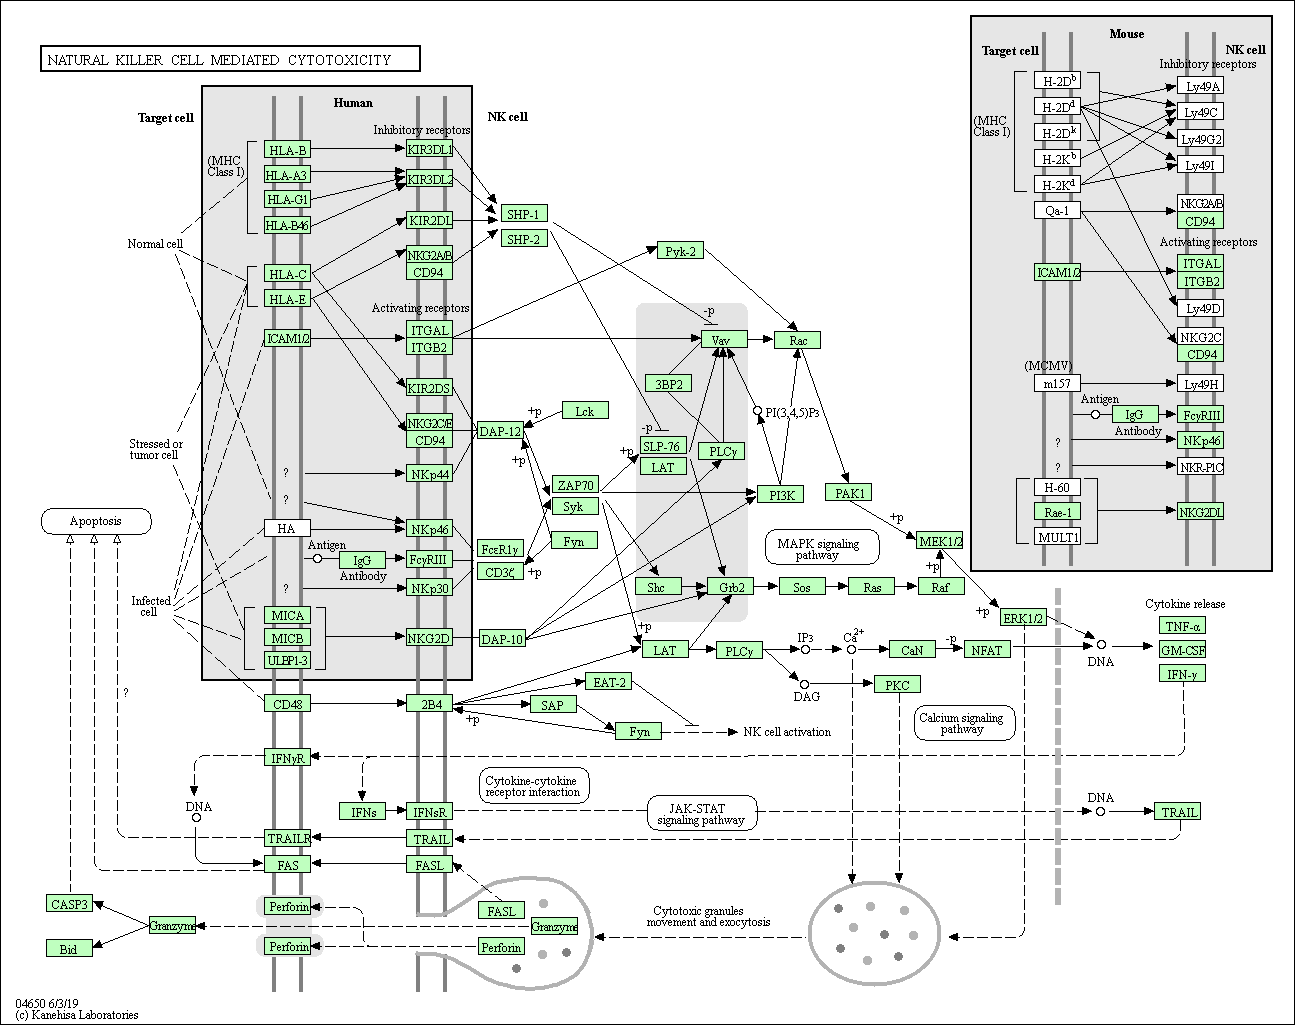
\includegraphics[width=0.8\linewidth]{results/7.KeggPathway/hsa04650} 

}

\caption{Cambios en los componentes biológicos implicados en la citotoxicidad de las células natural killer (KEGG ID: hsa04650) al comparar muestras ELI y SFI. Los componentes de color verde son sobre-expresados en ELI, mientras que los componentes rojos son infra-expresados. }\label{fig:Fig20}
\end{figure}

\newpage

\hypertarget{discusiuxf3n}{%
\section{5. Discusión}\label{discusiuxf3n}}

Los datos de \emph{RNA-Seq} de las muestras analizadas han permitido
obtener varios tránscripts con expresión diferencial entre los tipos de
infiltración comparados. A partir de la anotación de estos tránscripts,
se han obtenido distintas funciones biológicas que podrían estar
afectadas por el cambio de tipo de infiltración. En general, los
resultados concuerdan con lo que se esperaría a priori, ya que se
observa cierta tendencia a cambiar el metabolismo y activar la respuesta
immune al incrementar el tamaño de infiltración cancerígena.

Aún así, hay varios factores que es importante destacar que quizás han
afectado al análisis. En primer lugar, cabe tener en cuenta que con más
detalles de la función biológica a buscar o objetivo a conseguir se
podría haber elegido un filtrado más estricto. Aunque el \emph{p-valor}
de los contrastes se ajuste por BH, seguramente el filtrado más estricto
reduciria de forma más apropiada el error de tipo I, reduciendo así la
presencia de falsos positivos en el análisis de expresión diferencial.

En segundo lugar, tanto el análisis de similitud entre las muestras,
como el análisis de componentes principales o la visualización de
\emph{counts} para tránscripts individuales, dejan claro que la
agrupación de todas las muestras según tipo de infiltración no es del
todo claro a partir de los datos de los tránscripts. Por lo tanto, es
posible que si se selecionara un conjunto aleatorio de muestras
distinto, algunos de los resultados cambiaran. Sería interesante
intentar tomar un conjunto de muestras superior (más de 10 de cada
clase) para ver si los resultados se ven afectados. También podría ser
interesante tener en cuenta el sexo biologico del individuo, porqué
aunque solamente explique aproximadamente un \(10\%\) de la varianza
según el análisis de componentes principales, podría obtenerse unos
resultados más acurados.

Finalmente, también cabe destacar que casi la mitad de los tránscripts
no se pueden anotar. Así pues, es posible que haya un sesgo en el
análisis de significación biológica al obviar la actividad de un número
alto de tránscripts. Este análisis de significación biologica también
podría cambiar si se estudiaran solamente aquellos tránscripts con un
mínimo de efecto (por ejemplo, se podría aplicar el límite
\texttt{log2FoldChage\textgreater{}1} para estudiar aquellos tránscripts
cuya expresión fuera el doble entre condiciones).

En resumen, el estudio ha permitido relacionar los datos de
\emph{RNA-Seq} con cambios en la actividad biologica en función del tipo
de infiltración, pero se debería tener en cuenta que la seleción de
muestras, el filtrado de los datos, y la falta de anotaciones podría
afectar el resultado del análisis.

\newpage

\hypertarget{bibliografuxeda}{%
\section{6. Bibliografía}\label{bibliografuxeda}}

\hypertarget{refs}{}
\leavevmode\hypertarget{ref-hanzelmann2013gsva}{}%
Hänzelmann, Sonja, Robert Castelo, and Justin Guinney. 2013. ``GSVA:
Gene Set Variation Analysis for Microarray and Rna-Seq Data.'' \emph{BMC
Bioinformatics} 14 (1): 7.

\leavevmode\hypertarget{ref-lonsdale2013genotype}{}%
Lonsdale, John, Jeffrey Thomas, Mike Salvatore, Rebecca Phillips, Edmund
Lo, Saboor Shad, Richard Hasz, et al. 2013. ``The Genotype-Tissue
Expression (Gtex) Project.'' \emph{Nature Genetics} 45 (6): 580.

\leavevmode\hypertarget{ref-love2019analyzing}{}%
Love, Michael I, Simon Anders, and Wolfgang Huber. 2019. ``Analyzing
Rna-Seq Data with Deseq2.''

\leavevmode\hypertarget{ref-love2015rna}{}%
Love, Michael I, Simon Anders, Vladislav Kim, and Wolfgang Huber. 2015.
``RNA-Seq Workflow: Gene-Level Exploratory Analysis and Differential
Expression.'' \emph{F1000Research} 4.

\leavevmode\hypertarget{ref-morgan2017summarizedexperiment}{}%
Morgan, Martin, Valerie Obenchain, Jim Hester, and Hervé Pagès. 2017.
``SummarizedExperiment: SummarizedExperiment Container.'' \emph{R
Package Version} 1 (0).

\leavevmode\hypertarget{ref-phipson2016}{}%
Phipson, Belinda, Anna Trigos, Matt Ritchie, Maria Doyle, Harriet
Dashnow, and Charity Law. 2016. ``RNA-Seq Analysis in R: Differential
Expression Analysis.''
\url{https://combine-australia.github.io/RNAseq-R/06-rnaseq-day1.html}.

\leavevmode\hypertarget{ref-yu2012statistical}{}%
Yu, Guangchuang. 2012. ``Statistical Analysis and Visualization of
Functional Profiles for Genes and Gene Clusters.'' \emph{Journal of
Integrative Biology} 16 (5): 284--87.

\leavevmode\hypertarget{ref-yu2012clusterprofiler}{}%
Yu, Guangchuang, Li-Gen Wang, Yanyan Han, and Qing-Yu He. 2012.
``ClusterProfiler: An R Package for Comparing Biological Themes Among
Gene Clusters.'' \emph{Omics: A Journal of Integrative Biology} 16 (5):
284--87.

\leavevmode\hypertarget{ref-zhu2019heavy}{}%
Zhu, Anqi, Joseph G Ibrahim, and Michael I Love. 2019. ``Heavy-Tailed
Prior Distributions for Sequence Count Data: Removing the Noise and
Preserving Large Differences.'' \emph{Bioinformatics} 35 (12): 2084--92.

\newpage

\hypertarget{apuxe9ndice-cuxf3digo-de-r-y-obtenciuxf3n-de-resultados}{%
\section{7. Apéndice: Código de R y obtención de
resultados}\label{apuxe9ndice-cuxf3digo-de-r-y-obtenciuxf3n-de-resultados}}

\hypertarget{importar-y-preparar-los-datos}{%
\subsection{7.1. Importar y preparar los
datos}\label{importar-y-preparar-los-datos}}

Para recrear este trabajo será necesario un conjunto de librerías y
paquetes, para ello puede utilizarse el script adjunto
\texttt{InstallPackages.R}.

Para empezar, definimos el directorio de trabajo (que depende para cada
usuario) y creamos carpetas para guardar los datos y los resultados
producidos del análisis.

\begin{Shaded}
\begin{Highlighting}[]
\KeywordTok{setwd}\NormalTok{(}\StringTok{"C:/Users/Usuario/Documents/0.UOC/AnalisisOmicas/PEC2/exposit_marc_ADO_PEC2_MBio"}\NormalTok{)}
\KeywordTok{dir.create}\NormalTok{(}\StringTok{"data"}\NormalTok{)}
\KeywordTok{dir.create}\NormalTok{(}\StringTok{"results"}\NormalTok{)}
\end{Highlighting}
\end{Shaded}

A continuación, se descargan los datos del ejercicio y se descomprimen
en la carpeta \texttt{data}, para obtener los ficheros
\texttt{counts.csv} y \texttt{targets.csv} dentro de esta carpeta. Se
importan los dos ficheros completos como \texttt{data.frames} utilizando
\texttt{read.csv}.

\begin{Shaded}
\begin{Highlighting}[]
\NormalTok{counts <-}\StringTok{  }\KeywordTok{read.csv}\NormalTok{(}\StringTok{"./data/counts.csv"}\NormalTok{,}\DataTypeTok{header=}\NormalTok{T,}\DataTypeTok{sep=}\StringTok{";"}\NormalTok{, }\DataTypeTok{row.names=}\DecValTok{1}\NormalTok{)}
\NormalTok{targets <-}\StringTok{ }\KeywordTok{read.csv}\NormalTok{(}\StringTok{"./data/targets.csv"}\NormalTok{,}\DataTypeTok{header=}\NormalTok{T)}
\end{Highlighting}
\end{Shaded}

Para el análisis se utilizan solamente 10 muestras de cada uno de los
tres tipos (\texttt{NIT},\texttt{ELI},\texttt{SFI}). Para obtener el
subset podrían definirse conjuntos de cada una de las matrices
\texttt{counts} y \texttt{targets} y luego fusionarlas en un objeto
\texttt{DESeqDataSet} utilizando \texttt{DESeqDataSetFromMatrix}. Aún
así, siguiento esta aproximación hay riesgo de equivocarse al selecionar
\texttt{counts} y \texttt{targets} por separado y cruzar los
\texttt{counts} con la información de muestras distintas. Así pues, se
prefiere construir un objeto \texttt{SummarizedExperiment} con todos los
datos y después obtener un \texttt{subset} de indices para extraerlo del
objeto completo. Realizar subsets de \texttt{SummarizedExperiment}
resulta muy útil pues el objeto asegura que los counts y información de
cada muestra se mantienen correctamente.

Primero se construye el objeto \texttt{SummarizedExperiment} a partir de
los \texttt{data.frame} \texttt{counts} y \texttt{targets}. El objeto
\texttt{SummarizedExperiment} está construido por tres elementos
distintos. El objeto \texttt{colData} contiene información sobre las
muestras, el objeto \texttt{rowData} información sobre los genes, y el
objeto \texttt{assays} es la matriz de contajes obtenida al interceptar
\texttt{colData} con \texttt{rowData}. Esta matriz contiene el número de
\emph{reads} de cada gen (fila) en cada muestra (columna) obtenidos del
experimento de RNA-seq después de \emph{mapear} los \emph{reads}.

El objeto \texttt{counts} importado coincide con el objeto
\texttt{assays} del \texttt{SummarizedExperiment}, ya que cada columna
es una muestra distinta y cada fila un gen distinto, mientras que la
matriz tiene el número de \emph{reads} de cada gen en cada muestra. El
objeto \texttt{rowData} en este caso concuerda con la primera columna (o
identificador de fila) de la matriz de \texttt{counts}. Finalmente, el
objeto \texttt{targets} importado coincide con el objeto
\texttt{colData} de \texttt{SummarizedExperiment}, ya que cada fila
concuerda con las muestras de las columnas de la matriz de
\texttt{counts}.

Así se puede crear el objeto \texttt{SummarizedExperiment} a partir de
los datos importados. Hay 292 muestras y cada una tiene la información
de \texttt{counts} de 56202 genes. El objeto \texttt{rowData} solamente
contiene la información del ID del gen, mientras que \texttt{colData}
contiene información adicional de cada muestra, como un ID, el grupo de
la muestra o el tejido estudiado.

\begin{Shaded}
\begin{Highlighting}[]
\KeywordTok{library}\NormalTok{(}\StringTok{"BiocManager"}\NormalTok{)}
\KeywordTok{library}\NormalTok{(}\StringTok{"SummarizedExperiment"}\NormalTok{)}
\end{Highlighting}
\end{Shaded}

\begin{Shaded}
\begin{Highlighting}[]
\NormalTok{se <-}\StringTok{ }\KeywordTok{SummarizedExperiment}\NormalTok{(}\DataTypeTok{assays=}\KeywordTok{as.matrix}\NormalTok{(counts),}\DataTypeTok{colData=}\NormalTok{targets,}
                           \DataTypeTok{rowData=}\KeywordTok{list}\NormalTok{(}\DataTypeTok{gene_id=}\KeywordTok{row.names}\NormalTok{(counts)))}
\KeywordTok{assayNames}\NormalTok{(se) <-}\StringTok{ "counts"}
\NormalTok{se}
\end{Highlighting}
\end{Shaded}

\begin{verbatim}
## class: SummarizedExperiment 
## dim: 56202 292 
## metadata(0):
## assays(1): counts
## rownames(56202): ENSG00000223972.4 ENSG00000227232.4 ...
##   ENSG00000210195.2 ENSG00000210196.2
## rowData names(1): gene_id
## colnames(292): GTEX.111CU.0226.SM.5GZXC GTEX.111FC.1026.SM.5GZX1 ...
##   GTEX.ZZ64.0126.SM.5GZXA GTEX.ZZPU.1326.SM.5GZWS
## colData names(9): Experiment SRA_Sample ... Group ShortName
\end{verbatim}

Utilizando la información de \texttt{targets} puede verse que hay un
número distinto de muestras de cada clase. Para compararlas, se extraerá
solamente 10 muestras de cada grupo.

\begin{Shaded}
\begin{Highlighting}[]
\KeywordTok{table}\NormalTok{(targets}\OperatorTok{$}\NormalTok{Group)}
\end{Highlighting}
\end{Shaded}

\begin{verbatim}
## 
## ELI NIT SFI 
##  14 236  42
\end{verbatim}

Para ello, se deciden aleatoriamente 10 índices de la matriz cuyas
muestras pertenezcan a cada una de las clases. Se define una semilla
para que esta extracción sea aleatoria pero reproducible.

\begin{Shaded}
\begin{Highlighting}[]
\KeywordTok{set.seed}\NormalTok{(}\DecValTok{456}\NormalTok{)}
\NormalTok{id_nit <-}\StringTok{ }\KeywordTok{sample}\NormalTok{(}\KeywordTok{as.numeric}\NormalTok{(}\KeywordTok{row.names}\NormalTok{(targets[targets}\OperatorTok{$}\NormalTok{Group}\OperatorTok{==}\StringTok{"NIT"}\NormalTok{,])),}\DecValTok{10}\NormalTok{)}
\NormalTok{id_sfi <-}\StringTok{ }\KeywordTok{sample}\NormalTok{(}\KeywordTok{as.numeric}\NormalTok{(}\KeywordTok{row.names}\NormalTok{(targets[targets}\OperatorTok{$}\NormalTok{Group}\OperatorTok{==}\StringTok{"SFI"}\NormalTok{,])),}\DecValTok{10}\NormalTok{)}
\NormalTok{id_eli <-}\StringTok{ }\KeywordTok{sample}\NormalTok{(}\KeywordTok{as.numeric}\NormalTok{(}\KeywordTok{row.names}\NormalTok{(targets[targets}\OperatorTok{$}\NormalTok{Group}\OperatorTok{==}\StringTok{"ELI"}\NormalTok{,])),}\DecValTok{10}\NormalTok{)}
\end{Highlighting}
\end{Shaded}

Se comprueba que los índices obtenidos pertenezcan a muestras distintas
de cada una de las clases.

\begin{Shaded}
\begin{Highlighting}[]
\NormalTok{targets}\OperatorTok{$}\NormalTok{Group[id_nit]}
\end{Highlighting}
\end{Shaded}

\begin{verbatim}
##  [1] NIT NIT NIT NIT NIT NIT NIT NIT NIT NIT
## Levels: ELI NIT SFI
\end{verbatim}

\begin{Shaded}
\begin{Highlighting}[]
\NormalTok{targets}\OperatorTok{$}\NormalTok{Group[id_sfi]}
\end{Highlighting}
\end{Shaded}

\begin{verbatim}
##  [1] SFI SFI SFI SFI SFI SFI SFI SFI SFI SFI
## Levels: ELI NIT SFI
\end{verbatim}

\begin{Shaded}
\begin{Highlighting}[]
\NormalTok{targets}\OperatorTok{$}\NormalTok{Group[id_eli]}
\end{Highlighting}
\end{Shaded}

\begin{verbatim}
##  [1] ELI ELI ELI ELI ELI ELI ELI ELI ELI ELI
## Levels: ELI NIT SFI
\end{verbatim}

\begin{Shaded}
\begin{Highlighting}[]
\KeywordTok{dir.create}\NormalTok{(}\StringTok{"results/1.Filtraje"}\NormalTok{)}
\end{Highlighting}
\end{Shaded}

\begin{verbatim}
## Warning in dir.create("results/1.Filtraje"): 'results\1.Filtraje' already exists
\end{verbatim}

\begin{Shaded}
\begin{Highlighting}[]
\NormalTok{table_ids <-}\StringTok{ }\KeywordTok{matrix}\NormalTok{(}\OtherTok{NA}\NormalTok{,}\DataTypeTok{nrow=}\DecValTok{3}\NormalTok{,}\DataTypeTok{ncol=}\DecValTok{1}\NormalTok{)}
\NormalTok{table_ids[}\DecValTok{1}\NormalTok{] <-}\StringTok{ }\KeywordTok{paste}\NormalTok{(targets}\OperatorTok{$}\NormalTok{ShortName[id_nit],}\DataTypeTok{collapse=}\StringTok{", "}\NormalTok{)}
\NormalTok{table_ids[}\DecValTok{1}\NormalTok{] <-}\StringTok{ }\KeywordTok{paste0}\NormalTok{(}\KeywordTok{substr}\NormalTok{(table_ids[}\DecValTok{1}\NormalTok{],}\DecValTok{0}\NormalTok{,}\KeywordTok{nchar}\NormalTok{(table_ids[}\DecValTok{1}\NormalTok{])}\OperatorTok{/}\DecValTok{2}\NormalTok{),}\StringTok{"}\CharTok{\textbackslash{}n}\StringTok{"}\NormalTok{,}
                       \KeywordTok{substr}\NormalTok{(table_ids[}\DecValTok{1}\NormalTok{],}\KeywordTok{nchar}\NormalTok{(table_ids[}\DecValTok{1}\NormalTok{])}\OperatorTok{/}\DecValTok{2}\OperatorTok{+}\DecValTok{1}\NormalTok{,}\KeywordTok{nchar}\NormalTok{(table_ids[}\DecValTok{1}\NormalTok{])))}
\NormalTok{table_ids[}\DecValTok{2}\NormalTok{] <-}\StringTok{ }\KeywordTok{paste}\NormalTok{(targets}\OperatorTok{$}\NormalTok{ShortName[id_sfi],}\DataTypeTok{collapse=}\StringTok{", "}\NormalTok{)}
\NormalTok{table_ids[}\DecValTok{2}\NormalTok{] <-}\StringTok{ }\KeywordTok{paste0}\NormalTok{(}\KeywordTok{substr}\NormalTok{(table_ids[}\DecValTok{2}\NormalTok{],}\DecValTok{0}\NormalTok{,}\KeywordTok{nchar}\NormalTok{(table_ids[}\DecValTok{2}\NormalTok{])}\OperatorTok{/}\DecValTok{2}\NormalTok{),}\StringTok{"}\CharTok{\textbackslash{}n}\StringTok{"}\NormalTok{,}
                       \KeywordTok{substr}\NormalTok{(table_ids[}\DecValTok{2}\NormalTok{],}\KeywordTok{nchar}\NormalTok{(table_ids[}\DecValTok{2}\NormalTok{])}\OperatorTok{/}\DecValTok{2}\OperatorTok{+}\DecValTok{1}\NormalTok{,}\KeywordTok{nchar}\NormalTok{(table_ids[}\DecValTok{2}\NormalTok{])))}
\NormalTok{table_ids[}\DecValTok{3}\NormalTok{] <-}\StringTok{ }\KeywordTok{paste}\NormalTok{(targets}\OperatorTok{$}\NormalTok{ShortName[id_eli],}\DataTypeTok{collapse=}\StringTok{", "}\NormalTok{)}
\NormalTok{table_ids[}\DecValTok{3}\NormalTok{] <-}\StringTok{ }\KeywordTok{paste0}\NormalTok{(}\KeywordTok{substr}\NormalTok{(table_ids[}\DecValTok{3}\NormalTok{],}\DecValTok{0}\NormalTok{,}\KeywordTok{nchar}\NormalTok{(table_ids[}\DecValTok{3}\NormalTok{])}\OperatorTok{/}\DecValTok{2}\NormalTok{),}\StringTok{"}\CharTok{\textbackslash{}n}\StringTok{"}\NormalTok{,}
                       \KeywordTok{substr}\NormalTok{(table_ids[}\DecValTok{3}\NormalTok{],}\KeywordTok{nchar}\NormalTok{(table_ids[}\DecValTok{3}\NormalTok{])}\OperatorTok{/}\DecValTok{2}\OperatorTok{+}\DecValTok{1}\NormalTok{,}\KeywordTok{nchar}\NormalTok{(table_ids[}\DecValTok{3}\NormalTok{])))}
\KeywordTok{row.names}\NormalTok{(table_ids) <-}\StringTok{ }\KeywordTok{c}\NormalTok{(}\StringTok{"NIT"}\NormalTok{,}\StringTok{"SFI"}\NormalTok{,}\StringTok{"ELI"}\NormalTok{)}
\KeywordTok{save}\NormalTok{(table_ids, }\DataTypeTok{file=}\StringTok{"./results/1.Filtraje/SampInf.RDa"}\NormalTok{)}
\end{Highlighting}
\end{Shaded}

Finalmente, se extrae una subselección del objeto
\texttt{SummarizedExperiment} creado anteriormente a partir de los
índices definidos. La extracción de una subselección de
\texttt{SummarizedExperiment} es sencilla, pues la propia estructura del
objeto asegura que no se mezcla información de las muestras ni los
tránscritos. El objeto resultante contiene la información de todos los
tránscritos pero solamente con 10 muestras de cada grupo.

\begin{Shaded}
\begin{Highlighting}[]
\NormalTok{se_sub <-}\StringTok{ }\NormalTok{se[,}\KeywordTok{c}\NormalTok{(id_nit,id_sfi,id_eli)]}
\NormalTok{se_sub}
\end{Highlighting}
\end{Shaded}

\begin{verbatim}
## class: SummarizedExperiment 
## dim: 56202 30 
## metadata(0):
## assays(1): counts
## rownames(56202): ENSG00000223972.4 ENSG00000227232.4 ...
##   ENSG00000210195.2 ENSG00000210196.2
## rowData names(1): gene_id
## colnames(30): GTEX.ZY6K.0226.SM.5SIAY GTEX.T2IS.0626.SM.32QP6 ...
##   GTEX.11XUK.0226.SM.5EQLW GTEX.YFC4.2626.SM.5P9FQ
## colData names(9): Experiment SRA_Sample ... Group ShortName
\end{verbatim}

\begin{Shaded}
\begin{Highlighting}[]
\KeywordTok{table}\NormalTok{(se_sub}\OperatorTok{$}\NormalTok{Group)}
\end{Highlighting}
\end{Shaded}

\begin{verbatim}
## 
## ELI NIT SFI 
##  10  10  10
\end{verbatim}

Para realizar los análisis de \textbf{RNA-seq} se utilizarán las
funciones de la librería \texttt{DESeq2}, así que el objeto
\texttt{SummarizedExperiment} se transforma a \texttt{DESeqDataSet}. Se
especifica que los datos se analizarán según el grupo del experimento
(la condición utilizada). Nótese que para esto se reordena el orden de
los niveles del factor \texttt{Group}. Por defecto, en \texttt{R} el
valor númerico de los factores se asigna por orden alfabético, lo que
asignaría a \texttt{NIT} (la condición sin tratar) el nivel número 2,
mientras que por coherencia este debería ser el nivel 1. El nivel
\texttt{SFI} debería ser el segundo nivel por tener infiltración media y
el nivel \texttt{ELI} el tercero. Por esto, se recodifica la variable
\texttt{Group} indicando el orden de los factores (lo que no altera la
asignación de cada grupo)).

\begin{Shaded}
\begin{Highlighting}[]
\KeywordTok{library}\NormalTok{(}\StringTok{"DESeq2"}\NormalTok{)}
\end{Highlighting}
\end{Shaded}

\begin{Shaded}
\begin{Highlighting}[]
\NormalTok{se_sub}\OperatorTok{$}\NormalTok{Group <-}\StringTok{ }\KeywordTok{factor}\NormalTok{(se_sub}\OperatorTok{$}\NormalTok{Group,}\DataTypeTok{levels=}\KeywordTok{c}\NormalTok{(}\StringTok{"NIT"}\NormalTok{,}\StringTok{"SFI"}\NormalTok{,}\StringTok{"ELI"}\NormalTok{))}
\NormalTok{dds_unf <-}\StringTok{ }\KeywordTok{DESeqDataSet}\NormalTok{(se_sub, }\DataTypeTok{design =} \OperatorTok{~}\StringTok{ }\NormalTok{Group)}
\end{Highlighting}
\end{Shaded}

\hypertarget{control-de-calidad-y-filtraje}{%
\subsection{7.2. Control de calidad y
filtraje}\label{control-de-calidad-y-filtraje}}

El proceso de filtraje tiene por objetivo reducir el número de genes
contrastados estadísticamente, ya que el error de tipo I incrementa al
realizar un número elevado de comparaciones. Elegir el punto límite de
filtraje es delicado, ya que si se eliminaran demasiados genes podrían
perderse efectos importantes en el análisis.

Por este motivo, se prueba de aplicar distintos filtros para ver como
cambia el número de muestras estudiadas. Un filtrado básico es eliminar
aquellos genes cuyos tránscritos no se han identificado ni una sola vez
en ninguna de las 30 muestras comparadas (aquellos genes con
\texttt{counts=0}). También se suelen eliminar los genes con un solo
\texttt{count} ya que son igualmente poco importantes. Así, se puede ver
que hay 9950 genes sin ningún count y 2890 con un solo count entre todas
las muestras. Tras aplicar este filtrado básico el número de genes
comparados pasa de 56202 a 43362. A continuación, se prueba un filtrado
más \emph{agresivo}, que descartaría aquellos genes que no lleguen a 5
counts en almenos 10 muestras de las comparadas. Este filtro más
estricto o \texttt{strict} eliminaría 25229 genes del conjunto. Esto se
corresponde cerca del \(50\%\) de los datos.

En este caso, se toma \textbf{la decisión de mantener el filtro básico y
descartar aplicar un filtro que eliminaría el} \(50\%\) \textbf{de los
datos}. Seguramente, la información sobre el experimento y las preguntas
a responder permitiría saber si es preferible el error introducido al
comparar un elevado número de muestras o bien es preferible estudiar el
mayor número de genes posibles porqué es posible que haya interacciones.
Como no se dispone de esta información, se decide escoger la opción más
conservativa y menos riesgo de perder información. Aún así, el filtraje
realizado ya avanza que un gran número de los genes estudiados (cerca
del \(50\%\)) tiene un número de \texttt{counts} bajo (no llega ni a 5
counts en 10 de las muestras). Otro motivo por el que se ha optado por
un filtro suave es porqué al realizar el análisis de expresión
diferencial con \texttt{DESeq} esta función ya realiza un filtrado
simple.

\begin{Shaded}
\begin{Highlighting}[]
\KeywordTok{print}\NormalTok{(}\KeywordTok{paste0}\NormalTok{(}\StringTok{"Número de genes sin filtrar: "}\NormalTok{,}\KeywordTok{nrow}\NormalTok{(dds_unf)))}
\KeywordTok{print}\NormalTok{(}\KeywordTok{paste0}\NormalTok{(}\StringTok{"Número de genes con counts=0: "}\NormalTok{,}
             \KeywordTok{count}\NormalTok{(}\KeywordTok{rowSums}\NormalTok{(}\KeywordTok{counts}\NormalTok{(dds_unf))}\OperatorTok{==}\DecValTok{0}\NormalTok{)))}
\KeywordTok{print}\NormalTok{(}\KeywordTok{paste0}\NormalTok{(}\StringTok{"Número de genes con counts=1: "}\NormalTok{,}
             \KeywordTok{count}\NormalTok{(}\KeywordTok{rowSums}\NormalTok{(}\KeywordTok{counts}\NormalTok{(dds_unf))}\OperatorTok{==}\DecValTok{1}\NormalTok{)))}
\KeywordTok{print}\NormalTok{(}\KeywordTok{paste0}\NormalTok{(}\StringTok{"Número de genes con counts>=5 en >=10 muestras: "}\NormalTok{,}
             \KeywordTok{count}\NormalTok{(}\KeywordTok{rowSums}\NormalTok{(}\KeywordTok{counts}\NormalTok{(dds_unf) }\OperatorTok{>=}\StringTok{ }\DecValTok{5}\NormalTok{) }\OperatorTok{>=}\StringTok{ }\DecValTok{10}\NormalTok{)))}
\NormalTok{keep_sim <-}\StringTok{ }\KeywordTok{rowSums}\NormalTok{(}\KeywordTok{counts}\NormalTok{(dds_unf)) }\OperatorTok{>}\StringTok{ }\DecValTok{1}
\NormalTok{dds <-}\StringTok{ }\NormalTok{dds_unf[keep_sim,]}
\NormalTok{keep_str <-}\StringTok{ }\KeywordTok{rowSums}\NormalTok{(}\KeywordTok{counts}\NormalTok{(dds_unf) }\OperatorTok{>=}\StringTok{ }\DecValTok{5}\NormalTok{) }\OperatorTok{>=}\StringTok{ }\DecValTok{10}
\NormalTok{dds_str <-}\StringTok{ }\NormalTok{dds_unf[keep_str,]}
\KeywordTok{print}\NormalTok{(}\KeywordTok{paste0}\NormalTok{(}\StringTok{"Número de genes filtrando para counts>=1: "}\NormalTok{,}\KeywordTok{nrow}\NormalTok{(dds)))}
\end{Highlighting}
\end{Shaded}

\begin{verbatim}
## [1] "Número de genes sin filtrar: 56202"
## [1] "Número de genes con counts=0: 9950"
## [1] "Número de genes con counts=1: 2890"
## [1] "Número de genes con counts>=5 en >=10 muestras: 25229"
## [1] "Número de genes filtrando para counts>=1: 43362"
\end{verbatim}

El efecto de este filtro puede visualizarse observando como cambia la
distribución del número de contajes según las muestras. Para visualizar
la distribución del número de \emph{counts} se utiliza la transformación
VST, explicada más adelante. Así, se crean gráficos de densidad y
diagramas de caja que ilustran como se distribuyen los datos según el
filtraje aplicado. Aunque con el filtrado más agresivo se eliminen gran
parte de los datos con menor número de counts, se elige el más simple
para evitar perder efectos interesantes.

\begin{Shaded}
\begin{Highlighting}[]
\NormalTok{vsd_unf <-}\StringTok{ }\KeywordTok{vst}\NormalTok{(dds_unf, }\DataTypeTok{blind =} \OtherTok{FALSE}\NormalTok{)}
\NormalTok{vsd_sim <-}\StringTok{ }\KeywordTok{vst}\NormalTok{(dds, }\DataTypeTok{blind =} \OtherTok{FALSE}\NormalTok{)}
\NormalTok{vsd_str <-}\StringTok{ }\KeywordTok{vst}\NormalTok{(dds_str, }\DataTypeTok{blind =} \OtherTok{FALSE}\NormalTok{)}
\end{Highlighting}
\end{Shaded}

\begin{Shaded}
\begin{Highlighting}[]
\KeywordTok{png}\NormalTok{(}\StringTok{"results/1.Filtraje/1.FiltComp.png"}\NormalTok{,}\DataTypeTok{res =} \DecValTok{300}\NormalTok{,}\DataTypeTok{width =} \DecValTok{7}\NormalTok{,}\DataTypeTok{height =} \DecValTok{4}\NormalTok{, }\DataTypeTok{units =} \StringTok{'in'}\NormalTok{)}
\KeywordTok{par}\NormalTok{(}\DataTypeTok{mfrow=}\KeywordTok{c}\NormalTok{(}\DecValTok{1}\NormalTok{,}\DecValTok{3}\NormalTok{))}
\KeywordTok{boxplot}\NormalTok{(}\KeywordTok{assay}\NormalTok{(vsd_unf), }\DataTypeTok{xaxt=}\StringTok{'n'}\NormalTok{,}\DataTypeTok{xlab =} \StringTok{"Muestras"}\NormalTok{, }
        \DataTypeTok{ylab=}\StringTok{"Contaje normalizado por vst"}\NormalTok{, }\DataTypeTok{main=}\StringTok{"Sin filtrar"}\NormalTok{)}
\KeywordTok{axis}\NormalTok{(}\DecValTok{1}\NormalTok{, }\DataTypeTok{at=}\KeywordTok{seq}\NormalTok{(}\DecValTok{1}\NormalTok{,}\DecValTok{30}\NormalTok{))}
\KeywordTok{boxplot}\NormalTok{(}\KeywordTok{assay}\NormalTok{(vsd_sim), }\DataTypeTok{xaxt=}\StringTok{'n'}\NormalTok{,}\DataTypeTok{xlab =} \StringTok{"Muestras"}\NormalTok{, }
        \DataTypeTok{ylab=}\StringTok{"Contaje normalizado por vst"}\NormalTok{, }\DataTypeTok{main=}\StringTok{"Filtrado para counts>1"}\NormalTok{)}
\KeywordTok{axis}\NormalTok{(}\DecValTok{1}\NormalTok{, }\DataTypeTok{at=}\KeywordTok{seq}\NormalTok{(}\DecValTok{1}\NormalTok{,}\DecValTok{30}\NormalTok{))}
\KeywordTok{boxplot}\NormalTok{(}\KeywordTok{assay}\NormalTok{(vsd_str), }\DataTypeTok{xaxt=}\StringTok{'n'}\NormalTok{,}\DataTypeTok{xlab =} \StringTok{"Muestras"}\NormalTok{, }
        \DataTypeTok{ylab=}\StringTok{"Contaje normalizado por vst"}\NormalTok{, }\DataTypeTok{main=}\StringTok{"Flt. para cts>5 en 10 muestras"}\NormalTok{)}
\KeywordTok{axis}\NormalTok{(}\DecValTok{1}\NormalTok{, }\DataTypeTok{at=}\KeywordTok{seq}\NormalTok{(}\DecValTok{1}\NormalTok{,}\DecValTok{30}\NormalTok{))}
\KeywordTok{dev.off}\NormalTok{()}
\end{Highlighting}
\end{Shaded}

\begin{verbatim}
## pdf 
##   2
\end{verbatim}

\begin{Shaded}
\begin{Highlighting}[]
\KeywordTok{png}\NormalTok{(}\StringTok{"results/1.Filtraje/2.FiltDens.png"}\NormalTok{,}\DataTypeTok{res =} \DecValTok{300}\NormalTok{,}\DataTypeTok{width =} \DecValTok{7}\NormalTok{,}\DataTypeTok{height =} \DecValTok{4}\NormalTok{, }\DataTypeTok{units =} \StringTok{'in'}\NormalTok{)}
\KeywordTok{par}\NormalTok{(}\DataTypeTok{mfrow=}\KeywordTok{c}\NormalTok{(}\DecValTok{1}\NormalTok{,}\DecValTok{3}\NormalTok{))}
\KeywordTok{plot}\NormalTok{(}\KeywordTok{density}\NormalTok{(}\KeywordTok{assay}\NormalTok{(vsd_unf)[,}\DecValTok{1}\NormalTok{]), }\DataTypeTok{type =} \StringTok{"n"}\NormalTok{, }\DataTypeTok{main=}\StringTok{"Sin filtrar"}\NormalTok{,}
     \DataTypeTok{xlab=}\StringTok{"Counts normalizados"}\NormalTok{)}
\ControlFlowTok{for}\NormalTok{(i }\ControlFlowTok{in} \DecValTok{1}\OperatorTok{:}\NormalTok{(}\KeywordTok{dim}\NormalTok{(}\KeywordTok{assay}\NormalTok{(vsd_unf))[}\DecValTok{2}\NormalTok{]}\OperatorTok{-}\DecValTok{1}\NormalTok{))\{}
  \KeywordTok{lines}\NormalTok{(}\KeywordTok{density}\NormalTok{(}\KeywordTok{c}\NormalTok{(}\KeywordTok{assay}\NormalTok{(vsd_unf)[,i])))}
\NormalTok{\}}
\KeywordTok{plot}\NormalTok{(}\KeywordTok{density}\NormalTok{(}\KeywordTok{assay}\NormalTok{(vsd_sim)[,}\DecValTok{1}\NormalTok{]), }\DataTypeTok{type =} \StringTok{"n"}\NormalTok{, }\DataTypeTok{main=}\StringTok{"Filtrado para counts>1"}\NormalTok{,}
     \DataTypeTok{xlab=}\StringTok{"Counts normalizados"}\NormalTok{)}
\ControlFlowTok{for}\NormalTok{(i }\ControlFlowTok{in} \DecValTok{1}\OperatorTok{:}\NormalTok{(}\KeywordTok{dim}\NormalTok{(}\KeywordTok{assay}\NormalTok{(vsd_sim))[}\DecValTok{2}\NormalTok{]}\OperatorTok{-}\DecValTok{1}\NormalTok{))\{}
  \KeywordTok{lines}\NormalTok{(}\KeywordTok{density}\NormalTok{(}\KeywordTok{c}\NormalTok{(}\KeywordTok{assay}\NormalTok{(vsd_sim)[,i])))}
\NormalTok{\}}
\KeywordTok{plot}\NormalTok{(}\KeywordTok{density}\NormalTok{(}\KeywordTok{assay}\NormalTok{(vsd_str)[,}\DecValTok{1}\NormalTok{]), }\DataTypeTok{type =} \StringTok{"n"}\NormalTok{, }\DataTypeTok{main=}\StringTok{"Flt. para cts>5 en 10 muestras"}\NormalTok{,}
     \DataTypeTok{xlab=}\StringTok{"Counts normalizados"}\NormalTok{)}
\ControlFlowTok{for}\NormalTok{(i }\ControlFlowTok{in} \DecValTok{1}\OperatorTok{:}\NormalTok{(}\KeywordTok{dim}\NormalTok{(}\KeywordTok{assay}\NormalTok{(vsd_str))[}\DecValTok{2}\NormalTok{]}\OperatorTok{-}\DecValTok{1}\NormalTok{))\{}
  \KeywordTok{lines}\NormalTok{(}\KeywordTok{density}\NormalTok{(}\KeywordTok{c}\NormalTok{(}\KeywordTok{assay}\NormalTok{(vsd_str)[,i])))}
\NormalTok{\}}
\KeywordTok{dev.off}\NormalTok{()}
\end{Highlighting}
\end{Shaded}

\begin{verbatim}
## pdf 
##   2
\end{verbatim}

\hypertarget{exploraciuxf3n-descriptiva-de-las-muestras}{%
\subsection{7.3. Exploración descriptiva de las
muestras}\label{exploraciuxf3n-descriptiva-de-las-muestras}}

Para la exploración de datos multivariantes es importante asegurar la
homocedasticidad de los datos, es decir, que la varianza sea constante
independentmente de la media de las muestras. En el caso de los datos de
RNA-seq, la varianza incrementa con la media de cada muestra. Por esto,
para realizar análisis multivariantes con datos de RNA-seq es necesario
aplicar un proceso de normalización entre muestras que permita las
comparaciones.

Esta normalización se fundamenta en tomar el logaritmo de base 2
(\texttt{log2}) de los \emph{counts} al que se añade un pseudo-contaje
de 1 para evitar el caso \(log_2(0)=-\infty\). Aún así, esto incrementa
el peso que tienen los datos con bajos valores de \emph{counts} en estos
análisis multivariantes. Estos datos son precisamente aquellos con menos
separación entre señal y ruido y por lo tanto, podrían introduir ruido
en el análisis. Para solucionarlo, el paquete \texttt{DESeq} introduce
dos posibles transformaciones: la \emph{variance stabilizing
transformation} (VST) y la\emph{regularized-logarithm transformation}
(rlog).

Las dos transformaciones son prácticamente idénticas al \texttt{log2}
para valores altos, pero difieren en como tratan los valores pequeños.
Para muestras de tamaño medio y grande (n\textgreater=30) es más
adecuado utilizar \texttt{VST} ya que es más eficiente que
\texttt{rlog}, además es menos sensible a outliers de valores altos.
\textbf{Como en este caso hay 30 muestras, se utiliza la transformación
VST}.

\begin{Shaded}
\begin{Highlighting}[]
\NormalTok{vsd <-}\StringTok{ }\KeywordTok{vst}\NormalTok{(dds, }\DataTypeTok{blind =} \OtherTok{FALSE}\NormalTok{)}
\end{Highlighting}
\end{Shaded}

Con los datos transformados puede estudiarse la distribución de los
\emph{counts} según la muestra, tal y como se ha realizado anteriormente
en el proceso de filtraje. Aquí se reproducen el gráfico de densidad y
diagramas de cajas con los datos filtrados para counts\textgreater1, que
son los elegidos para el análisis.

\begin{Shaded}
\begin{Highlighting}[]
\KeywordTok{dir.create}\NormalTok{(}\StringTok{"results/2.AnaDescript"}\NormalTok{)}
\end{Highlighting}
\end{Shaded}

\begin{verbatim}
## Warning in dir.create("results/2.AnaDescript"): 'results\2.AnaDescript' already
## exists
\end{verbatim}

\begin{Shaded}
\begin{Highlighting}[]
\KeywordTok{png}\NormalTok{(}\StringTok{"results/2.AnaDescript/1.CountDist.png"}\NormalTok{,}\DataTypeTok{res =} \DecValTok{300}\NormalTok{,}\DataTypeTok{width=}\DecValTok{6}\NormalTok{,}\DataTypeTok{height=}\DecValTok{4}\NormalTok{,}\DataTypeTok{units=}\StringTok{'in'}\NormalTok{)}
\KeywordTok{par}\NormalTok{(}\DataTypeTok{mfrow=}\KeywordTok{c}\NormalTok{(}\DecValTok{1}\NormalTok{,}\DecValTok{2}\NormalTok{))}
\KeywordTok{boxplot}\NormalTok{(}\KeywordTok{assay}\NormalTok{(vsd), }\DataTypeTok{xaxt=}\StringTok{'n'}\NormalTok{,}\DataTypeTok{xlab=}\StringTok{"Muestras"}\NormalTok{, }\DataTypeTok{ylab=}\StringTok{"vst-normalized counts"}\NormalTok{,}
        \DataTypeTok{col =} \KeywordTok{c}\NormalTok{(}\KeywordTok{rep}\NormalTok{(}\StringTok{"red"}\NormalTok{, }\DecValTok{10}\NormalTok{), }\KeywordTok{rep}\NormalTok{(}\StringTok{"blue"}\NormalTok{, }\DecValTok{10}\NormalTok{), }\KeywordTok{rep}\NormalTok{(}\StringTok{"green"}\NormalTok{, }\DecValTok{10}\NormalTok{)))}
\KeywordTok{axis}\NormalTok{(}\DecValTok{1}\NormalTok{, }\DataTypeTok{at=}\KeywordTok{seq}\NormalTok{(}\DecValTok{1}\NormalTok{,}\DecValTok{30}\NormalTok{))}
\KeywordTok{plot}\NormalTok{(}\KeywordTok{density}\NormalTok{(}\KeywordTok{assay}\NormalTok{(vsd)[,}\DecValTok{1}\NormalTok{]), }\DataTypeTok{type =} \StringTok{"n"}\NormalTok{,}\DataTypeTok{xlab=}\StringTok{"vst-normalized counts"}\NormalTok{,}\DataTypeTok{main=}\StringTok{""}\NormalTok{)}
\ControlFlowTok{for}\NormalTok{(i }\ControlFlowTok{in} \DecValTok{1}\OperatorTok{:}\NormalTok{(}\KeywordTok{dim}\NormalTok{(}\KeywordTok{assay}\NormalTok{(vsd))[}\DecValTok{2}\NormalTok{]}\OperatorTok{-}\DecValTok{1}\NormalTok{))\{}
  \KeywordTok{lines}\NormalTok{(}\KeywordTok{density}\NormalTok{(}\KeywordTok{c}\NormalTok{(}\KeywordTok{assay}\NormalTok{(vsd)[,i])))}
\NormalTok{\}}
\KeywordTok{dev.off}\NormalTok{()}
\end{Highlighting}
\end{Shaded}

\begin{verbatim}
## pdf 
##   2
\end{verbatim}

Otras representaciones resultan más útiles para el estudio descriptivo
de las muestras. La primera de ellas es la representación de las
distancias entre las muestras estudiadas, que indica qué muestras son
similares entre ellas y cuales son distintas. Se espera observar las
muestras agrupadas en 3 grupos de 10 muestras según el tipo de
infiltración.

\begin{Shaded}
\begin{Highlighting}[]
\NormalTok{sampleDists <-}\StringTok{ }\KeywordTok{dist}\NormalTok{(}\KeywordTok{t}\NormalTok{(}\KeywordTok{assay}\NormalTok{(vsd)))}
\end{Highlighting}
\end{Shaded}

\begin{Shaded}
\begin{Highlighting}[]
\KeywordTok{library}\NormalTok{(}\StringTok{"pheatmap"}\NormalTok{)}
\KeywordTok{library}\NormalTok{(}\StringTok{"RColorBrewer"}\NormalTok{)}
\end{Highlighting}
\end{Shaded}

\begin{Shaded}
\begin{Highlighting}[]
\KeywordTok{png}\NormalTok{(}\StringTok{"results/2.AnaDescript/2.DistMuestras.png"}\NormalTok{,}\DataTypeTok{res=}\DecValTok{300}\NormalTok{,}\DataTypeTok{width=}\DecValTok{6}\NormalTok{,}\DataTypeTok{height=}\DecValTok{4}\NormalTok{,}\DataTypeTok{units=}\StringTok{'in'}\NormalTok{)}
\NormalTok{sampleDistMatrix <-}\StringTok{ }\KeywordTok{as.matrix}\NormalTok{(sampleDists)}
\KeywordTok{rownames}\NormalTok{(sampleDistMatrix) <-}\StringTok{ }\KeywordTok{paste}\NormalTok{(vsd}\OperatorTok{$}\NormalTok{Group,}\KeywordTok{colnames}\NormalTok{(vsd), }\DataTypeTok{sep=}\StringTok{" - "}\NormalTok{)}
\KeywordTok{colnames}\NormalTok{(sampleDistMatrix) <-}\StringTok{ }\OtherTok{NULL}
\NormalTok{colors <-}\StringTok{ }\KeywordTok{colorRampPalette}\NormalTok{(}\KeywordTok{rev}\NormalTok{(}\KeywordTok{brewer.pal}\NormalTok{(}\DecValTok{9}\NormalTok{, }\StringTok{"Blues"}\NormalTok{)) )(}\DecValTok{255}\NormalTok{)}
\KeywordTok{pheatmap}\NormalTok{(sampleDistMatrix,}
         \DataTypeTok{clustering_distance_rows =}\NormalTok{ sampleDists,}
         \DataTypeTok{clustering_distance_cols =}\NormalTok{ sampleDists,}
         \DataTypeTok{col =}\NormalTok{ colors, }\DataTypeTok{fontsize_row=}\DecValTok{7}\NormalTok{)}
\KeywordTok{dev.off}\NormalTok{()}
\end{Highlighting}
\end{Shaded}

\begin{verbatim}
## png 
##   3
\end{verbatim}

También es interesante estudiar la fuente de variabilidad de los datos a
través de un \emph{Principal Component Analysis} (PCA). Para ello, las
muestras se posicionan en un plano 2D en la dirección que explique la
mayor variabilidad en el eje X (dimensión 1) y en el eje Y la segunda
dimensión. Se elije visualizar el PCA de las muestras y representarlas
según el tipo de infiltración (\texttt{Group}) y sexo (\texttt{sex})
para añadir otra variable que podría ser de interés. Se utiliza
\texttt{ggplot} para poder distinguir las muestras con la forma para el
sexo y con el color para el grupo.

Se puede ver que el componentene principal explica un \(60\%\) de la
varianza y está bastante relacionado con el tipo de infiltración,
habiendo en un extremo \texttt{NIT} y en el otro \texttt{ELI}, con
\texttt{SFI} en medio, lo que concuerda con los tipos de infiltración.
La segunda componente explica una parte menor de la varianza, y tiene
que ver con el \texttt{sex} de los individuos ya que separa las muestras
en el eje vertical según esta variable.

\begin{Shaded}
\begin{Highlighting}[]
\NormalTok{pcaData <-}\StringTok{ }\KeywordTok{plotPCA}\NormalTok{(vsd, }\DataTypeTok{intgroup =} \KeywordTok{c}\NormalTok{( }\StringTok{"Group"}\NormalTok{, }\StringTok{"sex"}\NormalTok{), }\DataTypeTok{returnData =} \OtherTok{TRUE}\NormalTok{)}
\NormalTok{percentVar <-}\StringTok{ }\KeywordTok{round}\NormalTok{(}\DecValTok{100} \OperatorTok{*}\StringTok{ }\KeywordTok{attr}\NormalTok{(pcaData, }\StringTok{"percentVar"}\NormalTok{))}
\end{Highlighting}
\end{Shaded}

\begin{Shaded}
\begin{Highlighting}[]
\KeywordTok{library}\NormalTok{(ggplot2)}
\KeywordTok{png}\NormalTok{(}\StringTok{"results/2.AnaDescript/3.PCA.png"}\NormalTok{,}\DataTypeTok{res =} \DecValTok{300}\NormalTok{,}\DataTypeTok{width=}\DecValTok{6}\NormalTok{,}\DataTypeTok{height=}\DecValTok{4}\NormalTok{,}\DataTypeTok{units=}\StringTok{'in'}\NormalTok{)}
\KeywordTok{ggplot}\NormalTok{(pcaData, }\KeywordTok{aes}\NormalTok{(}\DataTypeTok{x =}\NormalTok{ PC1, }\DataTypeTok{y =}\NormalTok{ PC2, }\DataTypeTok{color =}\NormalTok{ Group, }\DataTypeTok{shape =}\NormalTok{ sex)) }\OperatorTok{+}
\StringTok{  }\KeywordTok{geom_point}\NormalTok{(}\DataTypeTok{size =}\DecValTok{3}\NormalTok{) }\OperatorTok{+}
\StringTok{  }\KeywordTok{xlab}\NormalTok{(}\KeywordTok{paste0}\NormalTok{(}\StringTok{"PC1: "}\NormalTok{, percentVar[}\DecValTok{1}\NormalTok{], }\StringTok{"% variance"}\NormalTok{)) }\OperatorTok{+}
\StringTok{  }\KeywordTok{ylab}\NormalTok{(}\KeywordTok{paste0}\NormalTok{(}\StringTok{"PC2: "}\NormalTok{, percentVar[}\DecValTok{2}\NormalTok{], }\StringTok{"% variance"}\NormalTok{)) }\OperatorTok{+}
\StringTok{  }\KeywordTok{coord_fixed}\NormalTok{() }\OperatorTok{+}
\StringTok{  }\KeywordTok{ggtitle}\NormalTok{(}\StringTok{"PCA con counts normalizados según sexo y grupo"}\NormalTok{)}
\KeywordTok{dev.off}\NormalTok{()}
\end{Highlighting}
\end{Shaded}

\begin{verbatim}
## pdf 
##   2
\end{verbatim}

\hypertarget{identificaciuxf3n-de-genes-diferencialmente-expresados}{%
\subsection{7.4. Identificación de genes diferencialmente
expresados}\label{identificaciuxf3n-de-genes-diferencialmente-expresados}}

La identificación de genes diferencialmente expresados
(\emph{differential expression analysis}) se realiza utilizando los
\emph{counts} sin normalizar por VST, ya que la función\texttt{DESeq}
tiene en cuenta el número de el tamaño de cada muestra y realiza una
normalización como paso inicial. Además, no es necesario especificar la
formula ya que se realizó al crear el objeto \texttt{DESeqDataSet},
indicando que se separaran las muestras según grupo (tipo de
infiltración).

\begin{Shaded}
\begin{Highlighting}[]
\NormalTok{dds <-}\StringTok{ }\KeywordTok{DESeq}\NormalTok{(dds)}
\end{Highlighting}
\end{Shaded}

\begin{verbatim}
## estimating size factors
\end{verbatim}

\begin{verbatim}
## estimating dispersions
\end{verbatim}

\begin{verbatim}
## gene-wise dispersion estimates
\end{verbatim}

\begin{verbatim}
## mean-dispersion relationship
\end{verbatim}

\begin{verbatim}
## final dispersion estimates
\end{verbatim}

\begin{verbatim}
## fitting model and testing
\end{verbatim}

\begin{verbatim}
## -- replacing outliers and refitting for 212 genes
## -- DESeq argument 'minReplicatesForReplace' = 7 
## -- original counts are preserved in counts(dds)
\end{verbatim}

\begin{verbatim}
## estimating dispersions
\end{verbatim}

\begin{verbatim}
## fitting model and testing
\end{verbatim}

El proceso indica que se han ajustado 212 genes que eran
\texttt{outliers}. Para verificar si alguna muestra contiene muchos
outliers y debería ser descartada para el análisis se utilizan las
distancias de Cook calculadas en el proceso de identificación de genes
diferencialmente expresados. A priori ya se informa que el número de
genes afectados es pequeño y por lo tanto no se debería ver ningúna
muestra que tenga un número tan alto de outliers que deba ser
descartada. El gráfico de las distancias de Cook indica que estas son
consistentes para todas las muestras, por lo que ninguna de las muestras
es consistentemente de valores diferentes a las otras, así que no hace
falta descartar ninguna.

\begin{Shaded}
\begin{Highlighting}[]
\KeywordTok{dir.create}\NormalTok{(}\StringTok{"results/3.ExpresionDiferencial"}\NormalTok{)}
\KeywordTok{png}\NormalTok{(}\StringTok{"results/3.ExpresionDiferencial/1.Outl.png"}\NormalTok{,}\DataTypeTok{res =} \DecValTok{300}\NormalTok{,}\DataTypeTok{width=}\DecValTok{6}\NormalTok{,}\DataTypeTok{height=}\DecValTok{4}\NormalTok{,}\DataTypeTok{units=}\StringTok{'in'}\NormalTok{)}
\KeywordTok{boxplot}\NormalTok{(}\KeywordTok{log10}\NormalTok{(}\KeywordTok{assays}\NormalTok{(dds)[[}\StringTok{"cooks"}\NormalTok{]]), }\DataTypeTok{range=}\DecValTok{0}\NormalTok{, }\DataTypeTok{las=}\DecValTok{2}\NormalTok{, }\DataTypeTok{xaxt=}\StringTok{'n'}\NormalTok{,}\DataTypeTok{xlab =} \StringTok{"Muestras"}\NormalTok{,}
        \DataTypeTok{ylab=}\StringTok{"Distancias de Cook"}\NormalTok{, }\DataTypeTok{col=}\KeywordTok{c}\NormalTok{(}\KeywordTok{rep}\NormalTok{(}\StringTok{"blue"}\NormalTok{,}\DecValTok{10}\NormalTok{),}\KeywordTok{rep}\NormalTok{(}\StringTok{"red"}\NormalTok{,}\DecValTok{10}\NormalTok{),}\KeywordTok{rep}\NormalTok{(}\StringTok{"green"}\NormalTok{,}\DecValTok{10}\NormalTok{)))}
\KeywordTok{axis}\NormalTok{(}\DecValTok{1}\NormalTok{, }\DataTypeTok{at=}\KeywordTok{seq}\NormalTok{(}\DecValTok{1}\NormalTok{,}\DecValTok{30}\NormalTok{))}
\KeywordTok{dev.off}\NormalTok{()}
\end{Highlighting}
\end{Shaded}

\begin{verbatim}
## pdf 
##   2
\end{verbatim}

Una vez se realiza el análisis de expresión diferencial, es necesario
extraer los resultados en tablas para cada comparación a realizar. En
este caso se realizan tres comparaciones: SFI-NIT, ELI-NIT, y ELI-SFI.

\begin{Shaded}
\begin{Highlighting}[]
\NormalTok{res_sfiNIT <-}\StringTok{ }\KeywordTok{results}\NormalTok{(dds, }\DataTypeTok{contrast=}\KeywordTok{c}\NormalTok{(}\StringTok{"Group"}\NormalTok{,}\StringTok{"SFI"}\NormalTok{,}\StringTok{"NIT"}\NormalTok{))}
\NormalTok{res_eliNIT <-}\StringTok{ }\KeywordTok{results}\NormalTok{(dds, }\DataTypeTok{contrast=}\KeywordTok{c}\NormalTok{(}\StringTok{"Group"}\NormalTok{,}\StringTok{"ELI"}\NormalTok{,}\StringTok{"NIT"}\NormalTok{))}
\NormalTok{res_eliSFI <-}\StringTok{ }\KeywordTok{results}\NormalTok{(dds, }\DataTypeTok{contrast=}\KeywordTok{c}\NormalTok{(}\StringTok{"Group"}\NormalTok{,}\StringTok{"ELI"}\NormalTok{,}\StringTok{"SFI"}\NormalTok{))}
\end{Highlighting}
\end{Shaded}

El objeto resultante contiene información en distintas columnas, como el
Fold Change de los genes en escala logarítmica de base 2 (tal y como se
hacía con los microarrays) y el p-valor de este efecto. Como se realizan
tantas comparaciones, se incluye un p-valor ajustado por
Benjamini-Hochberg (BH) para reducir el error de tipo I introducido al
comparar tantos genes. Los genes cuya expresión varie más entre muestras
son aquellos con mayor \texttt{log2FoldChange}, cambio que es
significante según el valor del \texttt{padj} que se asigna.

\begin{Shaded}
\begin{Highlighting}[]
\KeywordTok{mcols}\NormalTok{(res_sfiNIT)}
\end{Highlighting}
\end{Shaded}

\begin{verbatim}
## DataFrame with 6 rows and 2 columns
##                        type                               description
##                 <character>                               <character>
## baseMean       intermediate mean of normalized counts for all samples
## log2FoldChange      results  log2 fold change (MLE): Group SFI vs NIT
## lfcSE               results          standard error: Group SFI vs NIT
## stat                results          Wald statistic: Group SFI vs NIT
## pvalue              results       Wald test p-value: Group SFI vs NIT
## padj                results                      BH adjusted p-values
\end{verbatim}

El \texttt{summary} de cada tabla de resultados muestra datos
interesantes, como es el número de genes sobre-regulados o
infra-regulados con un \emph{p-value} ajustado menor de 0.1. En este
trabajo se consideran genes con expresión significativamente distinta
aceptando un \emph{False Discovery Rate} (FDR) del \(10\%\), así que se
consideran significativos aquellos que tienen un \emph{p-valor} ajustado
por Benjamini-Hochberg inferior a 0.1.

\begin{Shaded}
\begin{Highlighting}[]
\KeywordTok{summary}\NormalTok{(res_sfiNIT)}
\end{Highlighting}
\end{Shaded}

\begin{verbatim}
## 
## out of 43360 with nonzero total read count
## adjusted p-value < 0.1
## LFC > 0 (up)       : 158, 0.36%
## LFC < 0 (down)     : 39, 0.09%
## outliers [1]       : 0, 0%
## low counts [2]     : 18496, 43%
## (mean count < 4)
## [1] see 'cooksCutoff' argument of ?results
## [2] see 'independentFiltering' argument of ?results
\end{verbatim}

\begin{Shaded}
\begin{Highlighting}[]
\KeywordTok{summary}\NormalTok{(res_eliNIT)}
\end{Highlighting}
\end{Shaded}

\begin{verbatim}
## 
## out of 43360 with nonzero total read count
## adjusted p-value < 0.1
## LFC > 0 (up)       : 4597, 11%
## LFC < 0 (down)     : 2611, 6%
## outliers [1]       : 0, 0%
## low counts [2]     : 12612, 29%
## (mean count < 1)
## [1] see 'cooksCutoff' argument of ?results
## [2] see 'independentFiltering' argument of ?results
\end{verbatim}

\begin{Shaded}
\begin{Highlighting}[]
\KeywordTok{summary}\NormalTok{(res_eliSFI)}
\end{Highlighting}
\end{Shaded}

\begin{verbatim}
## 
## out of 43360 with nonzero total read count
## adjusted p-value < 0.1
## LFC > 0 (up)       : 4582, 11%
## LFC < 0 (down)     : 2732, 6.3%
## outliers [1]       : 0, 0%
## low counts [2]     : 13453, 31%
## (mean count < 1)
## [1] see 'cooksCutoff' argument of ?results
## [2] see 'independentFiltering' argument of ?results
\end{verbatim}

Se crea una tabla para visualizar estos datos para cada comparación.
Nótese que todos los datos parten del mismo número inicial de genes pero
se obtiene un número distinto de genes con expresión diferencial en cada
comparación.

\begin{Shaded}
\begin{Highlighting}[]
\NormalTok{tbl <-}\StringTok{ }\KeywordTok{data.frame}\NormalTok{(}\StringTok{"SFI-NIT"}\NormalTok{=}\OtherTok{NA}\NormalTok{,}\StringTok{"ELI-NIT"}\NormalTok{=}\OtherTok{NA}\NormalTok{,}\StringTok{"ELI-SFI"}\NormalTok{=}\OtherTok{NA}\NormalTok{)}
\NormalTok{tbl[}\DecValTok{1}\NormalTok{,}\DecValTok{1}\NormalTok{] <-}\StringTok{ }\KeywordTok{round}\NormalTok{(}\KeywordTok{sum}\NormalTok{(res_sfiNIT}\OperatorTok{$}\NormalTok{padj}\OperatorTok{<}\FloatTok{0.1} \OperatorTok{&}\StringTok{ }\NormalTok{res_sfiNIT}\OperatorTok{$}\NormalTok{log2FoldChange }\OperatorTok{>}\StringTok{ }\DecValTok{0}\NormalTok{,}\DataTypeTok{na.rm=}\NormalTok{T),}\DecValTok{0}\NormalTok{)}
\NormalTok{tbl[}\DecValTok{2}\NormalTok{,}\DecValTok{1}\NormalTok{] <-}\StringTok{ }\KeywordTok{paste}\NormalTok{(}\KeywordTok{round}\NormalTok{(}\KeywordTok{sum}\NormalTok{(res_sfiNIT}\OperatorTok{$}\NormalTok{padj}\OperatorTok{<}\FloatTok{0.1}\OperatorTok{&}\NormalTok{res_sfiNIT}\OperatorTok{$}\NormalTok{log2FoldChange }\OperatorTok{>}\StringTok{ }\DecValTok{0}\NormalTok{,}\DataTypeTok{na.rm=}\NormalTok{T)}
                        \OperatorTok{/}\KeywordTok{dim}\NormalTok{(res_sfiNIT)[}\DecValTok{1}\NormalTok{] }\OperatorTok{*}\DecValTok{100}\NormalTok{,}\DecValTok{2}\NormalTok{),}\StringTok{"%"}\NormalTok{,}\DataTypeTok{sep=}\StringTok{""}\NormalTok{)}
\NormalTok{tbl[}\DecValTok{3}\NormalTok{,}\DecValTok{1}\NormalTok{] <-}\StringTok{ }\KeywordTok{round}\NormalTok{(}\KeywordTok{sum}\NormalTok{(res_sfiNIT}\OperatorTok{$}\NormalTok{padj}\OperatorTok{<}\FloatTok{0.1} \OperatorTok{&}\StringTok{ }\NormalTok{res_sfiNIT}\OperatorTok{$}\NormalTok{log2FoldChange }\OperatorTok{<}\StringTok{ }\DecValTok{0}\NormalTok{,}\DataTypeTok{na.rm=}\NormalTok{T),}\DecValTok{0}\NormalTok{)}
\NormalTok{tbl[}\DecValTok{4}\NormalTok{,}\DecValTok{1}\NormalTok{] <-}\StringTok{ }\KeywordTok{paste}\NormalTok{(}\KeywordTok{round}\NormalTok{(}\KeywordTok{sum}\NormalTok{(res_sfiNIT}\OperatorTok{$}\NormalTok{padj}\OperatorTok{<}\FloatTok{0.1}\OperatorTok{&}\NormalTok{res_sfiNIT}\OperatorTok{$}\NormalTok{log2FoldChange}\OperatorTok{<}\DecValTok{0}\NormalTok{,}\DataTypeTok{na.rm=}\NormalTok{T)}
                        \OperatorTok{/}\KeywordTok{dim}\NormalTok{(res_sfiNIT)[}\DecValTok{1}\NormalTok{] }\OperatorTok{*}\DecValTok{100}\NormalTok{,}\DecValTok{2}\NormalTok{),}\StringTok{"%"}\NormalTok{,}\DataTypeTok{sep=}\StringTok{""}\NormalTok{)}
\NormalTok{tbl[}\DecValTok{1}\NormalTok{,}\DecValTok{2}\NormalTok{] <-}\StringTok{ }\KeywordTok{round}\NormalTok{(}\KeywordTok{sum}\NormalTok{(res_eliNIT}\OperatorTok{$}\NormalTok{padj}\OperatorTok{<}\FloatTok{0.1}\OperatorTok{&}\NormalTok{res_eliNIT}\OperatorTok{$}\NormalTok{log2FoldChange}\OperatorTok{>}\DecValTok{0}\NormalTok{,}\DataTypeTok{na.rm=}\NormalTok{T),}\DecValTok{0}\NormalTok{)}
\NormalTok{tbl[}\DecValTok{2}\NormalTok{,}\DecValTok{2}\NormalTok{] <-}\StringTok{ }\KeywordTok{paste}\NormalTok{(}\KeywordTok{round}\NormalTok{(}\KeywordTok{sum}\NormalTok{(res_eliNIT}\OperatorTok{$}\NormalTok{padj}\OperatorTok{<}\FloatTok{0.1} \OperatorTok{&}\StringTok{ }\NormalTok{res_eliNIT}\OperatorTok{$}\NormalTok{log2FoldChange}\OperatorTok{>}\DecValTok{0}\NormalTok{,}\DataTypeTok{na.rm=}\NormalTok{T)}
                        \OperatorTok{/}\KeywordTok{dim}\NormalTok{(res_eliNIT)[}\DecValTok{1}\NormalTok{] }\OperatorTok{*}\DecValTok{100}\NormalTok{,}\DecValTok{2}\NormalTok{),}\StringTok{"%"}\NormalTok{,}\DataTypeTok{sep=}\StringTok{""}\NormalTok{)}
\NormalTok{tbl[}\DecValTok{3}\NormalTok{,}\DecValTok{2}\NormalTok{] <-}\StringTok{ }\KeywordTok{round}\NormalTok{(}\KeywordTok{sum}\NormalTok{(res_eliNIT}\OperatorTok{$}\NormalTok{padj}\OperatorTok{<}\FloatTok{0.1} \OperatorTok{&}\StringTok{ }\NormalTok{res_eliNIT}\OperatorTok{$}\NormalTok{log2FoldChange }\OperatorTok{<}\StringTok{ }\DecValTok{0}\NormalTok{,}\DataTypeTok{na.rm=}\NormalTok{T),}\DecValTok{0}\NormalTok{)}
\NormalTok{tbl[}\DecValTok{4}\NormalTok{,}\DecValTok{2}\NormalTok{] <-}\StringTok{ }\KeywordTok{paste}\NormalTok{(}\KeywordTok{round}\NormalTok{(}\KeywordTok{sum}\NormalTok{(res_eliNIT}\OperatorTok{$}\NormalTok{padj}\OperatorTok{<}\FloatTok{0.1}\OperatorTok{&}\NormalTok{res_eliNIT}\OperatorTok{$}\NormalTok{log2FoldChange }\OperatorTok{<}\StringTok{ }\DecValTok{0}\NormalTok{,}\DataTypeTok{na.rm=}\NormalTok{T)}
                        \OperatorTok{/}\KeywordTok{dim}\NormalTok{(res_eliNIT)[}\DecValTok{1}\NormalTok{] }\OperatorTok{*}\DecValTok{100}\NormalTok{,}\DecValTok{2}\NormalTok{),}\StringTok{"%"}\NormalTok{,}\DataTypeTok{sep=}\StringTok{""}\NormalTok{)}
\NormalTok{tbl[}\DecValTok{1}\NormalTok{,}\DecValTok{3}\NormalTok{] <-}\StringTok{ }\KeywordTok{round}\NormalTok{(}\KeywordTok{sum}\NormalTok{(res_eliSFI}\OperatorTok{$}\NormalTok{padj}\OperatorTok{<}\FloatTok{0.1} \OperatorTok{&}\StringTok{ }\NormalTok{res_eliSFI}\OperatorTok{$}\NormalTok{log2FoldChange }\OperatorTok{>}\StringTok{ }\DecValTok{0}\NormalTok{,}\DataTypeTok{na.rm=}\NormalTok{T),}\DecValTok{0}\NormalTok{)}
\NormalTok{tbl[}\DecValTok{2}\NormalTok{,}\DecValTok{3}\NormalTok{] <-}\StringTok{ }\KeywordTok{paste}\NormalTok{(}\KeywordTok{round}\NormalTok{(}\KeywordTok{sum}\NormalTok{(res_eliSFI}\OperatorTok{$}\NormalTok{padj}\OperatorTok{<}\FloatTok{0.1} \OperatorTok{&}\StringTok{ }\NormalTok{res_eliSFI}\OperatorTok{$}\NormalTok{log2FoldChange}\OperatorTok{>}\DecValTok{0}\NormalTok{,}\DataTypeTok{na.rm=}\NormalTok{T)}
                        \OperatorTok{/}\KeywordTok{dim}\NormalTok{(res_eliSFI)[}\DecValTok{1}\NormalTok{] }\OperatorTok{*}\DecValTok{100}\NormalTok{,}\DecValTok{2}\NormalTok{),}\StringTok{"%"}\NormalTok{,}\DataTypeTok{sep=}\StringTok{""}\NormalTok{)}
\NormalTok{tbl[}\DecValTok{3}\NormalTok{,}\DecValTok{3}\NormalTok{] <-}\StringTok{ }\KeywordTok{round}\NormalTok{(}\KeywordTok{sum}\NormalTok{(res_eliSFI}\OperatorTok{$}\NormalTok{padj}\OperatorTok{<}\FloatTok{0.1} \OperatorTok{&}\StringTok{ }\NormalTok{res_eliSFI}\OperatorTok{$}\NormalTok{log2FoldChange}\OperatorTok{<}\DecValTok{0}\NormalTok{,}\DataTypeTok{na.rm=}\NormalTok{T),}\DecValTok{0}\NormalTok{)}
\NormalTok{tbl[}\DecValTok{4}\NormalTok{,}\DecValTok{3}\NormalTok{] <-}\StringTok{ }\KeywordTok{paste}\NormalTok{(}\KeywordTok{round}\NormalTok{(}\KeywordTok{sum}\NormalTok{(res_eliSFI}\OperatorTok{$}\NormalTok{padj}\OperatorTok{<}\FloatTok{0.1} \OperatorTok{&}\StringTok{ }\NormalTok{res_eliSFI}\OperatorTok{$}\NormalTok{log2FoldChange}\OperatorTok{<}\DecValTok{0}\NormalTok{,}\DataTypeTok{na.rm=}\NormalTok{T)}
                        \OperatorTok{/}\KeywordTok{dim}\NormalTok{(res_eliSFI)[}\DecValTok{1}\NormalTok{] }\OperatorTok{*}\DecValTok{100}\NormalTok{,}\DecValTok{2}\NormalTok{),}\StringTok{"%"}\NormalTok{,}\DataTypeTok{sep=}\StringTok{""}\NormalTok{)}

\KeywordTok{row.names}\NormalTok{(tbl) <-}\StringTok{ }\KeywordTok{c}\NormalTok{(}\StringTok{"Upregulated"}\NormalTok{,}\StringTok{"Upregulated (%)"}\NormalTok{,}\StringTok{"Downregulated"}\NormalTok{,}\StringTok{"Downregulated (%)"}\NormalTok{)}

\KeywordTok{save}\NormalTok{(tbl,}\DataTypeTok{file=}\StringTok{"./results/3.ExpresionDiferencial/Reslt_summary.Rda"}\NormalTok{)}
\end{Highlighting}
\end{Shaded}

\hypertarget{anotaciuxf3n-de-los-resultados-2}{%
\subsection{7.5. Anotación de los
resultados}\label{anotaciuxf3n-de-los-resultados-2}}

Antes de presentar la lista de los genes expresados diferencialmente, se
anotan a partir de sus identidades. La tabla de resultados tiene para
cada fila el identificador del gen estudiado siguiendo el codigo de
\texttt{Ensembl\ gene\ ID}, que indica el codigo de transcript. Nótese
que el código de cada ID tiene el codigo seguido por un punto y un
número que indica la versión. Para enlazarlos con los datos de anotación
se tiene en cuenta solamente el geneID sin la versión indicada tras el
punto. como los geneID tienen 15 carácteres se utilizan solamente los
primeros 15 carácteres de cada uno. El órden de los ID es el mismo en
todas las comparaciones, así que se crea un solo vector.

\begin{Shaded}
\begin{Highlighting}[]
\NormalTok{ens.str <-}\StringTok{ }\KeywordTok{substr}\NormalTok{(}\KeywordTok{rownames}\NormalTok{(res_eliNIT), }\DecValTok{1}\NormalTok{, }\DecValTok{15}\NormalTok{)}
\KeywordTok{head}\NormalTok{(}\KeywordTok{rownames}\NormalTok{(res_eliNIT))}
\end{Highlighting}
\end{Shaded}

\begin{verbatim}
## [1] "ENSG00000223972.4" "ENSG00000227232.4" "ENSG00000243485.2"
## [4] "ENSG00000237613.2" "ENSG00000268020.2" "ENSG00000240361.1"
\end{verbatim}

\begin{Shaded}
\begin{Highlighting}[]
\KeywordTok{head}\NormalTok{(ens.str)}
\end{Highlighting}
\end{Shaded}

\begin{verbatim}
## [1] "ENSG00000223972" "ENSG00000227232" "ENSG00000243485" "ENSG00000237613"
## [5] "ENSG00000268020" "ENSG00000240361"
\end{verbatim}

Para realizar las anotaciones se utiliza el paquete de anotaciones de
Ensembl de Bioconductor, \texttt{org.Hs.eg.db}. Para relacionar el
codigo de cada transcript en cada fila con el resto de sus datos se
utiliza la función \texttt{mapIds}. Se juntan a la tabla una columna con
el símbolo del gen (\texttt{symbol}) que es una abreviatura del nombre
del gen, el Enterez ID y el nombre completo del gen al que pertenece el
transcript. Nótese que casi la mitad de transcripts no se pueden anotar
con un gene ID, ya que no todos los transcripts están anotados en la
base de datos de Ensembl.

\begin{Shaded}
\begin{Highlighting}[]
\KeywordTok{library}\NormalTok{(}\StringTok{"AnnotationDbi"}\NormalTok{)}
\end{Highlighting}
\end{Shaded}

\begin{verbatim}
## 
## Attaching package: 'AnnotationDbi'
\end{verbatim}

\begin{verbatim}
## The following object is masked from 'package:dplyr':
## 
##     select
\end{verbatim}

\begin{Shaded}
\begin{Highlighting}[]
\KeywordTok{library}\NormalTok{(}\StringTok{"org.Hs.eg.db"}\NormalTok{)}
\end{Highlighting}
\end{Shaded}

\begin{verbatim}
## 
\end{verbatim}

\begin{Shaded}
\begin{Highlighting}[]
\NormalTok{res_eliNIT}\OperatorTok{$}\NormalTok{symbol <-}\StringTok{ }\KeywordTok{mapIds}\NormalTok{(org.Hs.eg.db,}\DataTypeTok{keys=}\NormalTok{ens.str,}
                     \DataTypeTok{column=}\StringTok{"SYMBOL"}\NormalTok{,}\DataTypeTok{keytype=}\StringTok{"ENSEMBL"}\NormalTok{,}\DataTypeTok{multiVals=}\StringTok{"first"}\NormalTok{)}
\NormalTok{res_eliNIT}\OperatorTok{$}\NormalTok{entrez <-}\StringTok{ }\KeywordTok{mapIds}\NormalTok{(org.Hs.eg.db,}\DataTypeTok{keys=}\NormalTok{ens.str,}
                     \DataTypeTok{column=}\StringTok{"ENTREZID"}\NormalTok{,}\DataTypeTok{keytype=}\StringTok{"ENSEMBL"}\NormalTok{,}\DataTypeTok{multiVals=}\StringTok{"first"}\NormalTok{)}
\NormalTok{res_eliNIT}\OperatorTok{$}\NormalTok{gname <-}\StringTok{ }\KeywordTok{mapIds}\NormalTok{(org.Hs.eg.db,}\DataTypeTok{keys=}\NormalTok{ens.str,}
                    \DataTypeTok{column=}\StringTok{"GENENAME"}\NormalTok{,}\DataTypeTok{keytype=}\StringTok{"ENSEMBL"}\NormalTok{,}\DataTypeTok{multiVals=}\StringTok{"first"}\NormalTok{)}

\NormalTok{res_eliSFI}\OperatorTok{$}\NormalTok{symbol <-}\StringTok{ }\KeywordTok{mapIds}\NormalTok{(org.Hs.eg.db,}\DataTypeTok{keys=}\NormalTok{ens.str,}
                     \DataTypeTok{column=}\StringTok{"SYMBOL"}\NormalTok{,}\DataTypeTok{keytype=}\StringTok{"ENSEMBL"}\NormalTok{,}\DataTypeTok{multiVals=}\StringTok{"first"}\NormalTok{)}
\NormalTok{res_eliSFI}\OperatorTok{$}\NormalTok{entrez <-}\StringTok{ }\KeywordTok{mapIds}\NormalTok{(org.Hs.eg.db,}\DataTypeTok{keys=}\NormalTok{ens.str,}
                     \DataTypeTok{column=}\StringTok{"ENTREZID"}\NormalTok{,}\DataTypeTok{keytype=}\StringTok{"ENSEMBL"}\NormalTok{,}\DataTypeTok{multiVals=}\StringTok{"first"}\NormalTok{)}
\NormalTok{res_eliSFI}\OperatorTok{$}\NormalTok{gname <-}\StringTok{ }\KeywordTok{mapIds}\NormalTok{(org.Hs.eg.db,}\DataTypeTok{keys=}\NormalTok{ens.str,}
                    \DataTypeTok{column=}\StringTok{"GENENAME"}\NormalTok{,}\DataTypeTok{keytype=}\StringTok{"ENSEMBL"}\NormalTok{,}\DataTypeTok{multiVals=}\StringTok{"first"}\NormalTok{)}

\NormalTok{res_sfiNIT}\OperatorTok{$}\NormalTok{symbol <-}\StringTok{ }\KeywordTok{mapIds}\NormalTok{(org.Hs.eg.db,}\DataTypeTok{keys=}\NormalTok{ens.str,}
                     \DataTypeTok{column=}\StringTok{"SYMBOL"}\NormalTok{,}\DataTypeTok{keytype=}\StringTok{"ENSEMBL"}\NormalTok{,}\DataTypeTok{multiVals=}\StringTok{"first"}\NormalTok{)}
\NormalTok{res_sfiNIT}\OperatorTok{$}\NormalTok{entrez <-}\StringTok{ }\KeywordTok{mapIds}\NormalTok{(org.Hs.eg.db,}\DataTypeTok{keys=}\NormalTok{ens.str,}
                     \DataTypeTok{column=}\StringTok{"ENTREZID"}\NormalTok{,}\DataTypeTok{keytype=}\StringTok{"ENSEMBL"}\NormalTok{,}\DataTypeTok{multiVals=}\StringTok{"first"}\NormalTok{)}
\NormalTok{res_sfiNIT}\OperatorTok{$}\NormalTok{gname <-}\StringTok{ }\KeywordTok{mapIds}\NormalTok{(org.Hs.eg.db,}\DataTypeTok{keys=}\NormalTok{ens.str,}
                    \DataTypeTok{column=}\StringTok{"GENENAME"}\NormalTok{,}\DataTypeTok{keytype=}\StringTok{"ENSEMBL"}\NormalTok{,}\DataTypeTok{multiVals=}\StringTok{"first"}\NormalTok{)}
\KeywordTok{sum}\NormalTok{(}\KeywordTok{is.na}\NormalTok{(res_eliNIT}\OperatorTok{$}\NormalTok{entrez))}
\end{Highlighting}
\end{Shaded}

\begin{verbatim}
## [1] 20860
\end{verbatim}

Con los datos anotados se crean tablas para mostrar los 6 tránscritos
más sobre- y infra- regulados de cada grupo con mayor cambio de
regulación (mayor \texttt{log2FoldChange}) y significancia al \(90\%\).
Se añade para cada tránscrito información el \texttt{log2FoldChange}
(efecto del gen), el p-valor ajustado (\texttt{padj}), el nombre
abreviado del gen al que pertenece y su entrez ID. Nótese que se
muestran los tránscritos significativos con mayor cambio de expresión,
que no es lo mismo que mostrar los tránscritos con mayor nivel de
significación. Para ello, se crea primero un objeto que contenga
solamente los tránscritos significativos, y luego se ordenan según el
\texttt{log2FoldChange}.

\begin{Shaded}
\begin{Highlighting}[]
\NormalTok{resSig_sfiNIT <-}\StringTok{ }\KeywordTok{subset}\NormalTok{(res_sfiNIT, padj }\OperatorTok{<}\StringTok{ }\FloatTok{0.1}\NormalTok{)}
\NormalTok{resSig_eliNIT <-}\StringTok{ }\KeywordTok{subset}\NormalTok{(res_eliNIT, padj }\OperatorTok{<}\StringTok{ }\FloatTok{0.1}\NormalTok{)}
\NormalTok{resSig_eliSFI <-}\StringTok{ }\KeywordTok{subset}\NormalTok{(res_eliSFI, padj }\OperatorTok{<}\StringTok{ }\FloatTok{0.1}\NormalTok{)}
\end{Highlighting}
\end{Shaded}

\begin{Shaded}
\begin{Highlighting}[]
\NormalTok{factorsToShow <-}\StringTok{ }\KeywordTok{c}\NormalTok{(}\StringTok{"log2FoldChange"}\NormalTok{,}\StringTok{"padj"}\NormalTok{,}\StringTok{"symbol"}\NormalTok{,}\StringTok{"entrez"}\NormalTok{,}\StringTok{"gname"}\NormalTok{)}

\NormalTok{SvNDwn <-}\StringTok{ }\KeywordTok{head}\NormalTok{(resSig_sfiNIT[}\KeywordTok{order}\NormalTok{(resSig_sfiNIT}\OperatorTok{$}\NormalTok{log2FoldChange),factorsToShow])}
\NormalTok{SvNUp <-}\StringTok{ }\KeywordTok{head}\NormalTok{(resSig_sfiNIT[}\KeywordTok{order}\NormalTok{(resSig_sfiNIT}\OperatorTok{$}\NormalTok{log2FoldChange,}\DataTypeTok{decreasing=}\NormalTok{T),}
\NormalTok{                            factorsToShow])}
\NormalTok{EvNDwn <-}\StringTok{ }\KeywordTok{head}\NormalTok{(resSig_eliNIT[}\KeywordTok{order}\NormalTok{(resSig_eliNIT}\OperatorTok{$}\NormalTok{log2FoldChange),factorsToShow])}
\NormalTok{EvNUp <-}\StringTok{ }\KeywordTok{head}\NormalTok{(resSig_eliNIT[}\KeywordTok{order}\NormalTok{(resSig_eliNIT}\OperatorTok{$}\NormalTok{log2FoldChange,}\DataTypeTok{decreasing=}\NormalTok{T),}
\NormalTok{                            factorsToShow])}
\NormalTok{EvSDwn <-}\StringTok{ }\KeywordTok{head}\NormalTok{(resSig_eliSFI[}\KeywordTok{order}\NormalTok{(resSig_eliSFI}\OperatorTok{$}\NormalTok{log2FoldChange),factorsToShow])}
\NormalTok{EvSUp <-}\StringTok{ }\KeywordTok{head}\NormalTok{(resSig_eliSFI[}\KeywordTok{order}\NormalTok{(resSig_eliSFI}\OperatorTok{$}\NormalTok{log2FoldChange,}\DataTypeTok{decreasing=}\NormalTok{T),}
\NormalTok{                            factorsToShow])}
\KeywordTok{save}\NormalTok{(SvNDwn,}\DataTypeTok{file=}\StringTok{"./results/3.ExpresionDiferencial/Reslt_SvNDwn.Rda"}\NormalTok{)}
\KeywordTok{save}\NormalTok{(SvNUp,}\DataTypeTok{file=}\StringTok{"./results/3.ExpresionDiferencial/Reslt_SvNUp.Rda"}\NormalTok{)}
\KeywordTok{save}\NormalTok{(EvNDwn,}\DataTypeTok{file=}\StringTok{"./results/3.ExpresionDiferencial/Reslt_EvNDwn.Rda"}\NormalTok{)}
\KeywordTok{save}\NormalTok{(EvNUp,}\DataTypeTok{file=}\StringTok{"./results/3.ExpresionDiferencial/Reslt_EvNUp.Rda"}\NormalTok{)}
\KeywordTok{save}\NormalTok{(EvSDwn,}\DataTypeTok{file=}\StringTok{"./results/3.ExpresionDiferencial/Reslt_EvSDwn.Rda"}\NormalTok{)}
\KeywordTok{save}\NormalTok{(EvSUp,}\DataTypeTok{file=}\StringTok{"./results/3.ExpresionDiferencial/Reslt_EvSUp.Rda"}\NormalTok{)}
\end{Highlighting}
\end{Shaded}

\hypertarget{visualizaciuxf3n-de-genes-diferencialmente-expresados}{%
\subsection{7.6. Visualización de genes diferencialmente
expresados}\label{visualizaciuxf3n-de-genes-diferencialmente-expresados}}

Con los resultados de expresión diferencial de genes anotados se pueden
crear múltiples visualizaciones. La más simple de ellas es la
visualización del número de contajes de un tránscript en concreto según
el grupo de la muestra. Para ello, seleccionamos dos tránscritos
distintos. El tránscript ENSG00000100721.6 se encuentra entre los 6
genes más sobre-regulados al comparar ELI-NIT o ELI-SFI, pero no para la
comparación SFI-NIT. El tránscript ENSG00000100604.8 se encuentra
infra-regulado al comparar EFI-SFI o EFI-NIT, pero no para SFI-NIT.

\begin{Shaded}
\begin{Highlighting}[]
\NormalTok{UpRGene <-}\StringTok{ }\KeywordTok{rownames}\NormalTok{(EvNUp)[}\DecValTok{2}\NormalTok{]}
\NormalTok{UpRGene }\OperatorTok\StringTok{ }\KeywordTok{rownames}\NormalTok{(EvSUp)}
\end{Highlighting}
\end{Shaded}

\begin{verbatim}
## [1] TRUE
\end{verbatim}

\begin{Shaded}
\begin{Highlighting}[]
\NormalTok{UpRGene }\OperatorTok\StringTok{ }\KeywordTok{rownames}\NormalTok{(SvNUp)}
\end{Highlighting}
\end{Shaded}

\begin{verbatim}
## [1] FALSE
\end{verbatim}

\begin{Shaded}
\begin{Highlighting}[]
\NormalTok{DwRGene <-}\StringTok{ }\KeywordTok{rownames}\NormalTok{(EvSDwn)[}\DecValTok{3}\NormalTok{]}
\NormalTok{DwRGene }\OperatorTok\StringTok{ }\KeywordTok{rownames}\NormalTok{(EvNDwn)}
\end{Highlighting}
\end{Shaded}

\begin{verbatim}
## [1] TRUE
\end{verbatim}

\begin{Shaded}
\begin{Highlighting}[]
\NormalTok{DwRGene }\OperatorTok\StringTok{ }\KeywordTok{rownames}\NormalTok{(SvNDwn)}
\end{Highlighting}
\end{Shaded}

\begin{verbatim}
## [1] FALSE
\end{verbatim}

La función \texttt{plotCounts} permite ver que efectivamente el
tránscript ENSG00000100721.6 está sobre-expresado en \texttt{EFI}
respeto las otras dos comparaciones, mientras que el tránscript
ENSG00000100604.8 está infra-expresado en \texttt{EFI} respeto las otras
dos comparaciones.

\begin{Shaded}
\begin{Highlighting}[]
\KeywordTok{dir.create}\NormalTok{(}\StringTok{"results/4.DEAnl"}\NormalTok{)}
\KeywordTok{png}\NormalTok{(}\StringTok{"results/4.DEAnl/1.CntsTOP.png"}\NormalTok{,}\DataTypeTok{res =} \DecValTok{300}\NormalTok{,}\DataTypeTok{width=}\DecValTok{7}\NormalTok{,}\DataTypeTok{height=}\DecValTok{4}\NormalTok{,}\DataTypeTok{units=}\StringTok{'in'}\NormalTok{)}
\KeywordTok{par}\NormalTok{(}\DataTypeTok{mfrow=}\KeywordTok{c}\NormalTok{(}\DecValTok{1}\NormalTok{,}\DecValTok{2}\NormalTok{))}
\KeywordTok{plotCounts}\NormalTok{(dds,}\DataTypeTok{gene =}\NormalTok{ UpRGene, }\DataTypeTok{intgroup =} \KeywordTok{c}\NormalTok{(}\StringTok{"Group"}\NormalTok{))}
\KeywordTok{plotCounts}\NormalTok{(dds,}\DataTypeTok{gene =}\NormalTok{ DwRGene, }\DataTypeTok{intgroup =} \KeywordTok{c}\NormalTok{(}\StringTok{"Group"}\NormalTok{))}
\KeywordTok{dev.off}\NormalTok{()}
\end{Highlighting}
\end{Shaded}

\begin{verbatim}
## pdf 
##   2
\end{verbatim}

Esta opción permite representar de forma simple los \texttt{counts} para
un conjunto de genes definido. A continuación, se muestra como ejemplo
la lista de los genes con mayor efecto de sobre-regulación en la
comparación entre ELI-NIT. Se puede ver que el nivel de SFI está en un
término intermedio entre los dos niveles \texttt{ELI} y \texttt{NIT} en
la mayoría de estos tránscripts.

\begin{Shaded}
\begin{Highlighting}[]
\KeywordTok{png}\NormalTok{(}\StringTok{"results/4.DEAnl/2.CntsEvN.png"}\NormalTok{,}\DataTypeTok{res =} \DecValTok{300}\NormalTok{,}\DataTypeTok{width=}\DecValTok{8}\NormalTok{,}\DataTypeTok{height=}\DecValTok{5}\NormalTok{,}\DataTypeTok{units=}\StringTok{'in'}\NormalTok{)}
\KeywordTok{par}\NormalTok{(}\DataTypeTok{mfrow=}\KeywordTok{c}\NormalTok{(}\DecValTok{2}\NormalTok{,}\DecValTok{3}\NormalTok{))}
\ControlFlowTok{for}\NormalTok{ (i }\ControlFlowTok{in} \KeywordTok{seq}\NormalTok{(}\DecValTok{1}\NormalTok{,}\DecValTok{6}\NormalTok{))\{}
  \KeywordTok{plotCounts}\NormalTok{(dds,}\DataTypeTok{gene =} \KeywordTok{rownames}\NormalTok{(EvNUp)[i], }\DataTypeTok{intgroup =} \KeywordTok{c}\NormalTok{(}\StringTok{"Group"}\NormalTok{))}
\NormalTok{\}}
\KeywordTok{dev.off}\NormalTok{()}
\end{Highlighting}
\end{Shaded}

\begin{verbatim}
## pdf 
##   2
\end{verbatim}

Otra opción son los gráficos MA para observar la distribución de los
coeficientes del modelo (el cambio de expresión, log2FC) según las
comparaciones realizadas. Los gráficos MA muestran los cambios del
log2FC atribuibles a cierta variable a lo largo de la media de los
counts normalizadas para todas las muestras. Para su correcta generación
se elimina el ruido de log2FC asociado a los genes con bajo número de
counts a través del estrechamiento o \emph{shrinkage} de los valores de
log2FC. Por esto, se utiliza la función \texttt{lfcShrink} y se genera
un nuevo objeto con los resultados.

\begin{Shaded}
\begin{Highlighting}[]
\KeywordTok{library}\NormalTok{(}\StringTok{"apeglm"}\NormalTok{)}
\end{Highlighting}
\end{Shaded}

\begin{Shaded}
\begin{Highlighting}[]
\NormalTok{resMAP_sfiNIT <-}\StringTok{ }\KeywordTok{lfcShrink}\NormalTok{(dds,}\DataTypeTok{coef=}\StringTok{"Group_SFI_vs_NIT"}\NormalTok{,}\DataTypeTok{type=}\StringTok{"apeglm"}\NormalTok{)}
\NormalTok{resMAP_eliNIT <-}\StringTok{ }\KeywordTok{lfcShrink}\NormalTok{(dds,}\DataTypeTok{coef=}\StringTok{"Group_ELI_vs_NIT"}\NormalTok{,}\DataTypeTok{type=}\StringTok{"apeglm"}\NormalTok{)}
\end{Highlighting}
\end{Shaded}

Con el ruido de log2FC eliminado, se representan los gráficos MA para
las comparaciones SFI-NIT y ELI-NIT. La comparación restante entre
SFI-ELI no se realiza, puesto que no está immediatamente disponible del
objeto \texttt{dds}, que solamente compara los dos grupos con el grupo
base definido aquí como \texttt{NIT}. Para realizarse debería aplicarse
una transformación \texttt{normal} o \texttt{ashr} en vez de
\texttt{apeglm}, ya que las otras funciones permiten añadir diseños
arbitrarios. Esto no se hace aquí para simplificar, puesto que los
valores de log2FC obtenidos serían diferentes a los de las otras dos
comparaciones.

\begin{Shaded}
\begin{Highlighting}[]
\KeywordTok{resultsNames}\NormalTok{(dds)}
\end{Highlighting}
\end{Shaded}

\begin{verbatim}
## [1] "Intercept"        "Group_SFI_vs_NIT" "Group_ELI_vs_NIT"
\end{verbatim}

La función \texttt{plotMA} se utiliza para representar los gráficos MA
de las comparaciones SFI-NIT y ELI-NIT. Para cada una de ellas, se
señaliza el gen con un mayor p-valor ajustado, que como puede verse en
el eje vertical no tiene porqué ser el gen con mayor FC. Nótese el
significado de los puntos, que son rojos si para este gen en concreto el
p-valor ajustado es significante al \(10\%\) de significancia. También
se indican con un tríangulo los valores que caen fuera del eje vertical
representado en el gráfico.

\begin{Shaded}
\begin{Highlighting}[]
\KeywordTok{png}\NormalTok{(}\StringTok{"results/4.DEAnl/3.MASvN.png"}\NormalTok{,}\DataTypeTok{res =} \DecValTok{300}\NormalTok{,}\DataTypeTok{width=}\FloatTok{4.5}\NormalTok{,}\DataTypeTok{height=}\DecValTok{4}\NormalTok{,}\DataTypeTok{units=}\StringTok{'in'}\NormalTok{)}
\KeywordTok{plotMA}\NormalTok{(resMAP_sfiNIT, }\DataTypeTok{ylim=}\KeywordTok{c}\NormalTok{(}\OperatorTok{-}\DecValTok{7}\NormalTok{,}\DecValTok{7}\NormalTok{),}\DataTypeTok{main=}\StringTok{"MA plot for SFI-NIT"}\NormalTok{)}
\NormalTok{topGene1 <-}\StringTok{ }\KeywordTok{rownames}\NormalTok{(res_sfiNIT)[}\KeywordTok{which.min}\NormalTok{(res_sfiNIT}\OperatorTok{$}\NormalTok{padj)]}
\KeywordTok{with}\NormalTok{(resMAP_sfiNIT[topGene1, ], \{}
  \KeywordTok{points}\NormalTok{(baseMean, log2FoldChange, }\DataTypeTok{col=}\StringTok{"dodgerblue"}\NormalTok{, }\DataTypeTok{cex=}\DecValTok{2}\NormalTok{, }\DataTypeTok{lwd=}\DecValTok{2}\NormalTok{)}
  \KeywordTok{text}\NormalTok{(baseMean, log2FoldChange, topGene1, }\DataTypeTok{pos=}\DecValTok{2}\NormalTok{, }\DataTypeTok{col=}\StringTok{"dodgerblue"}\NormalTok{)}
\NormalTok{\})}
\KeywordTok{dev.off}\NormalTok{()}
\end{Highlighting}
\end{Shaded}

\begin{verbatim}
## pdf 
##   2
\end{verbatim}

\begin{Shaded}
\begin{Highlighting}[]
\KeywordTok{png}\NormalTok{(}\StringTok{"results/4.DEAnl/4.MAEvN.png"}\NormalTok{,}\DataTypeTok{res =} \DecValTok{300}\NormalTok{,}\DataTypeTok{width=}\FloatTok{4.5}\NormalTok{,}\DataTypeTok{height=}\DecValTok{4}\NormalTok{,}\DataTypeTok{units=}\StringTok{'in'}\NormalTok{)}
\KeywordTok{plotMA}\NormalTok{(resMAP_eliNIT, }\DataTypeTok{ylim=}\KeywordTok{c}\NormalTok{(}\OperatorTok{-}\DecValTok{10}\NormalTok{,}\DecValTok{10}\NormalTok{),}\DataTypeTok{main=}\StringTok{"MA plot for ELI-NIT"}\NormalTok{)}
\NormalTok{topGene2 <-}\StringTok{ }\KeywordTok{rownames}\NormalTok{(res_eliNIT)[}\KeywordTok{which.min}\NormalTok{(res_eliNIT}\OperatorTok{$}\NormalTok{padj)]}
\KeywordTok{with}\NormalTok{(resMAP_eliNIT[topGene2, ], \{}
  \KeywordTok{points}\NormalTok{(baseMean, log2FoldChange, }\DataTypeTok{col=}\StringTok{"dodgerblue"}\NormalTok{, }\DataTypeTok{cex=}\DecValTok{2}\NormalTok{, }\DataTypeTok{lwd=}\DecValTok{2}\NormalTok{)}
  \KeywordTok{text}\NormalTok{(baseMean, log2FoldChange, topGene2, }\DataTypeTok{pos=}\DecValTok{3}\NormalTok{, }\DataTypeTok{col=}\StringTok{"dodgerblue"}\NormalTok{)}
\NormalTok{\})}
\KeywordTok{dev.off}\NormalTok{()}
\end{Highlighting}
\end{Shaded}

\begin{verbatim}
## pdf 
##   2
\end{verbatim}

Los resultados del análisis de expresión diferencial permiten agrupar
los tránscritos según su valor en cada muestra en función del grupo,
para visualizar relaciones interesantes. De forma similar a como se hizo
para agrupar las muestras según sus varianzas, se pueden agrupar las
muestras y sus genes expresados diferencialmente. Para ello, se
seleccionan los 20 genes con más expresión diferencial entre las
muestras estudiadas y se representan por grupos. Nótese que se trabaja
con los datos normalizados por VST. En el \emph{heatmap} resultante
puede verse como cambia el nivel de grupos de genes según el tipo de
infiltración de la muestra, lo que puede revelar algun tipo de relación
biológica entre las actividades de estos tránscripts relacionados.
También es interesante ver que el efecto del sexo es claro en las
relaciones.

\begin{Shaded}
\begin{Highlighting}[]
\KeywordTok{png}\NormalTok{(}\StringTok{"results/4.DEAnl/5.Heatmap.png"}\NormalTok{,}\DataTypeTok{res =} \DecValTok{300}\NormalTok{,}\DataTypeTok{width=}\DecValTok{7}\NormalTok{,}\DataTypeTok{height=}\DecValTok{4}\NormalTok{,}\DataTypeTok{units=}\StringTok{'in'}\NormalTok{)}
\NormalTok{topVarGenes <-}\StringTok{ }\KeywordTok{head}\NormalTok{(}\KeywordTok{order}\NormalTok{(}\KeywordTok{rowVars}\NormalTok{(}\KeywordTok{assay}\NormalTok{(vsd)), }\DataTypeTok{decreasing =} \OtherTok{TRUE}\NormalTok{), }\DecValTok{20}\NormalTok{)}
\NormalTok{topGenes <-}\StringTok{ }\KeywordTok{assay}\NormalTok{(vsd)[topVarGenes, ]}
\NormalTok{topGenes <-}\StringTok{ }\NormalTok{topGenes }\OperatorTok{-}\StringTok{ }\KeywordTok{rowMeans}\NormalTok{(topGenes)}
\NormalTok{annot <-}\StringTok{ }\KeywordTok{as.data.frame}\NormalTok{(}\KeywordTok{colData}\NormalTok{(vsd)[,}\KeywordTok{c}\NormalTok{(}\StringTok{"Group"}\NormalTok{,}\StringTok{"sex"}\NormalTok{)])}
\KeywordTok{pheatmap}\NormalTok{(topGenes, }\DataTypeTok{annotation_col =}\NormalTok{ annot,}\DataTypeTok{fontsize=}\DecValTok{5}\NormalTok{)}
\KeywordTok{dev.off}\NormalTok{()}
\end{Highlighting}
\end{Shaded}

\begin{verbatim}
## png 
##   3
\end{verbatim}

Finalmente, pueden representarse los datos en un \emph{Volcano Plot}, es
decir, según su \texttt{log2FoldChange} que indica el nivel del efecto y
si es sobre- o infra- expresión y según su \emph{p-valor} ajustado que
indica la significancia de este cambio. Como ejemplo se representan los
tránscripts de la comparación ELI-NIT, indicando aquellos con cambio
significativo (p-valor ajustado\textless0.1) en color azul y añadiendo
el nombre de los 5 tránscripts con un menor p-valor.

\begin{Shaded}
\begin{Highlighting}[]
\KeywordTok{library}\NormalTok{(ggrepel)}
\NormalTok{res_eliNIT}\OperatorTok{$}\NormalTok{threshold <-}\StringTok{ }\NormalTok{res_eliNIT}\OperatorTok{$}\NormalTok{padj }\OperatorTok{<}\StringTok{ }\FloatTok{0.1}
\NormalTok{res_eliNIT_ord <-}\StringTok{ }\NormalTok{res_eliNIT[}\KeywordTok{order}\NormalTok{(res_eliNIT}\OperatorTok{$}\NormalTok{padj),] }
\NormalTok{res_eliNIT_ord}\OperatorTok{$}\NormalTok{genelabels <-}\StringTok{ ""}
\NormalTok{res_eliNIT_ord}\OperatorTok{$}\NormalTok{genelabels[}\DecValTok{1}\OperatorTok{:}\DecValTok{5}\NormalTok{] <-}\StringTok{ }\KeywordTok{rownames}\NormalTok{(res_eliNIT_ord)[}\DecValTok{1}\OperatorTok{:}\DecValTok{5}\NormalTok{]}


\KeywordTok{png}\NormalTok{(}\StringTok{"results/4.DEAnl/6.VolcPl.png"}\NormalTok{,}\DataTypeTok{res =} \DecValTok{300}\NormalTok{,}\DataTypeTok{width=}\FloatTok{4.5}\NormalTok{,}\DataTypeTok{height=}\DecValTok{4}\NormalTok{,}\DataTypeTok{units=}\StringTok{'in'}\NormalTok{)}
\KeywordTok{ggplot}\NormalTok{(}\KeywordTok{na.omit}\NormalTok{(}\KeywordTok{as.data.frame}\NormalTok{(res_eliNIT_ord))) }\OperatorTok{+}
\StringTok{  }\KeywordTok{geom_point}\NormalTok{(}\KeywordTok{aes}\NormalTok{(}\DataTypeTok{x =}\NormalTok{ log2FoldChange, }\DataTypeTok{y =} \OperatorTok{-}\KeywordTok{log10}\NormalTok{(padj), }\DataTypeTok{colour =}\NormalTok{ threshold)) }\OperatorTok{+}\StringTok{ }
\StringTok{  }\KeywordTok{geom_text_repel}\NormalTok{(}\KeywordTok{aes}\NormalTok{(}\DataTypeTok{x =}\NormalTok{ log2FoldChange, }\DataTypeTok{y =} \OperatorTok{-}\KeywordTok{log10}\NormalTok{(padj),}
                      \DataTypeTok{label=}\KeywordTok{ifelse}\NormalTok{(genelabels}\OperatorTok{==}\StringTok{""}\NormalTok{,}\StringTok{""}\NormalTok{,}\KeywordTok{rownames}\NormalTok{(res_eliNIT_ord)))) }\OperatorTok{+}
\StringTok{  }\KeywordTok{ggtitle}\NormalTok{(}\StringTok{"Expresión diferencial en ELI-NIT"}\NormalTok{) }\OperatorTok{+}
\StringTok{  }\KeywordTok{xlab}\NormalTok{(}\StringTok{"log2 Fold Change"}\NormalTok{) }\OperatorTok{+}\StringTok{ }
\StringTok{  }\KeywordTok{ylab}\NormalTok{(}\StringTok{"-log10 p-valor ajustado"}\NormalTok{) }\OperatorTok{+}
\StringTok{  }\KeywordTok{theme}\NormalTok{(}\DataTypeTok{legend.position =} \StringTok{"none"}\NormalTok{,}
        \DataTypeTok{plot.title =} \KeywordTok{element_text}\NormalTok{(}\DataTypeTok{size =} \KeywordTok{rel}\NormalTok{(}\FloatTok{1.5}\NormalTok{), }\DataTypeTok{hjust =} \FloatTok{0.5}\NormalTok{),}
        \DataTypeTok{axis.title =} \KeywordTok{element_text}\NormalTok{(}\DataTypeTok{size =} \KeywordTok{rel}\NormalTok{(}\FloatTok{1.25}\NormalTok{))) }
\KeywordTok{dev.off}\NormalTok{()}
\end{Highlighting}
\end{Shaded}

\begin{verbatim}
## pdf 
##   2
\end{verbatim}

\hypertarget{agrupaciuxf3n-de-las-comparaciones}{%
\subsection{7.7. Agrupación de las
comparaciones}\label{agrupaciuxf3n-de-las-comparaciones}}

No hay suficiente con comparar muestras a pares para entender totalmente
los datos. Para ello, es necesario comparar distintas comparaciones
entre ellas y ver qué genes se encuentra expresados diferencialmente en
común entre estos grupos, tiniendo en cuenta si están sobre- o infra-
regulados. Para esta visualización se utiliza un diagrama de Venn.

Para aprovechar la función \texttt{vennDiagram} del paquete
\texttt{limma} se construye \emph{manualmente} una matriz que indica si
un gen es significativo al \(10\%\) y sobre-expresado (+1) o
infra-expresado (-1) o bien si no es significativo y/o expresado
diferencialmente (0), para cada comparación.

\begin{Shaded}
\begin{Highlighting}[]
\KeywordTok{dir.create}\NormalTok{(}\StringTok{"results/5.CompComp"}\NormalTok{)}
\NormalTok{vennreslt <-}\StringTok{ }\KeywordTok{matrix}\NormalTok{(}\OtherTok{NA}\NormalTok{,}\DataTypeTok{nrow =} \KeywordTok{nrow}\NormalTok{(res_eliNIT), }\DataTypeTok{ncol=}\DecValTok{3}\NormalTok{)}

\NormalTok{nonSig <-}\StringTok{ }\NormalTok{(res_sfiNIT[,}\StringTok{"padj"}\NormalTok{] }\OperatorTok{>=}\StringTok{ }\FloatTok{0.1} \OperatorTok{|}\StringTok{ }\KeywordTok{is.na}\NormalTok{(res_sfiNIT[,}\StringTok{"padj"}\NormalTok{]))}
\NormalTok{UpReg <-}\StringTok{ }\OperatorTok{!}\NormalTok{nonSig }\OperatorTok{&}\StringTok{ }\NormalTok{res_sfiNIT[,}\StringTok{"log2FoldChange"}\NormalTok{] }\OperatorTok{>}\StringTok{ }\DecValTok{0}
\NormalTok{DwReg <-}\StringTok{ }\OperatorTok{!}\NormalTok{nonSig }\OperatorTok{&}\StringTok{ }\NormalTok{res_sfiNIT[,}\StringTok{"log2FoldChange"}\NormalTok{] }\OperatorTok{<}\StringTok{ }\DecValTok{0}
\NormalTok{vennreslt[nonSig,}\DecValTok{1}\NormalTok{] <-}\StringTok{ }\DecValTok{0} 
\NormalTok{vennreslt[UpReg,}\DecValTok{1}\NormalTok{] <-}\StringTok{ }\OperatorTok{+}\DecValTok{1}
\NormalTok{vennreslt[DwReg,}\DecValTok{1}\NormalTok{] <-}\StringTok{ }\DecValTok{-1}

\NormalTok{nonSig <-}\StringTok{ }\NormalTok{(res_eliNIT[,}\StringTok{"padj"}\NormalTok{] }\OperatorTok{>=}\StringTok{ }\FloatTok{0.1} \OperatorTok{|}\StringTok{ }\KeywordTok{is.na}\NormalTok{(res_eliNIT[,}\StringTok{"padj"}\NormalTok{]))}
\NormalTok{UpReg <-}\StringTok{ }\OperatorTok{!}\NormalTok{nonSig }\OperatorTok{&}\StringTok{ }\NormalTok{res_eliNIT[,}\StringTok{"log2FoldChange"}\NormalTok{] }\OperatorTok{>}\StringTok{ }\DecValTok{0}
\NormalTok{DwReg <-}\StringTok{ }\OperatorTok{!}\NormalTok{nonSig }\OperatorTok{&}\StringTok{ }\NormalTok{res_eliNIT[,}\StringTok{"log2FoldChange"}\NormalTok{] }\OperatorTok{<}\StringTok{ }\DecValTok{0}
\NormalTok{vennreslt[nonSig,}\DecValTok{2}\NormalTok{] <-}\StringTok{ }\DecValTok{0} 
\NormalTok{vennreslt[UpReg,}\DecValTok{2}\NormalTok{] <-}\StringTok{ }\OperatorTok{+}\DecValTok{1}
\NormalTok{vennreslt[DwReg,}\DecValTok{2}\NormalTok{] <-}\StringTok{ }\DecValTok{-1}

\NormalTok{nonSig <-}\StringTok{ }\NormalTok{(res_eliSFI[,}\StringTok{"padj"}\NormalTok{] }\OperatorTok{>=}\StringTok{ }\FloatTok{0.1} \OperatorTok{|}\StringTok{ }\KeywordTok{is.na}\NormalTok{(res_eliSFI[,}\StringTok{"padj"}\NormalTok{]))}
\NormalTok{UpReg <-}\StringTok{ }\OperatorTok{!}\NormalTok{nonSig }\OperatorTok{&}\StringTok{ }\NormalTok{res_eliSFI[,}\StringTok{"log2FoldChange"}\NormalTok{] }\OperatorTok{>}\StringTok{ }\DecValTok{0}
\NormalTok{DwReg <-}\StringTok{ }\OperatorTok{!}\NormalTok{nonSig }\OperatorTok{&}\StringTok{ }\NormalTok{res_eliSFI[,}\StringTok{"log2FoldChange"}\NormalTok{] }\OperatorTok{<}\StringTok{ }\DecValTok{0}
\NormalTok{vennreslt[nonSig,}\DecValTok{3}\NormalTok{] <-}\StringTok{ }\DecValTok{0} 
\NormalTok{vennreslt[UpReg,}\DecValTok{3}\NormalTok{] <-}\StringTok{ }\OperatorTok{+}\DecValTok{1}
\NormalTok{vennreslt[DwReg,}\DecValTok{3}\NormalTok{] <-}\StringTok{ }\DecValTok{-1}

\KeywordTok{colnames}\NormalTok{(vennreslt) <-}\StringTok{ }\KeywordTok{c}\NormalTok{(}\StringTok{"SFI-NIT"}\NormalTok{,}\StringTok{"ELI-NIT"}\NormalTok{,}\StringTok{"ELI-SFI"}\NormalTok{)}
\end{Highlighting}
\end{Shaded}

Con la matriz puede representarse el diagrama de Venn, que compara las
distintas comparaciones entre ellas.

\begin{Shaded}
\begin{Highlighting}[]
\KeywordTok{library}\NormalTok{(limma)}
\end{Highlighting}
\end{Shaded}

\begin{verbatim}
## 
## Attaching package: 'limma'
\end{verbatim}

\begin{verbatim}
## The following object is masked from 'package:DESeq2':
## 
##     plotMA
\end{verbatim}

\begin{verbatim}
## The following object is masked from 'package:BiocGenerics':
## 
##     plotMA
\end{verbatim}

\begin{Shaded}
\begin{Highlighting}[]
\KeywordTok{png}\NormalTok{(}\StringTok{"results/5.CompComp/1.Venn.png"}\NormalTok{,}\DataTypeTok{res =} \DecValTok{300}\NormalTok{,}\DataTypeTok{width=}\FloatTok{4.5}\NormalTok{,}\DataTypeTok{height=}\DecValTok{4}\NormalTok{,}\DataTypeTok{units=}\StringTok{'in'}\NormalTok{)}
\KeywordTok{vennDiagram}\NormalTok{(vennreslt, }\DataTypeTok{include=}\KeywordTok{c}\NormalTok{(}\StringTok{"up"}\NormalTok{,}\StringTok{"down"}\NormalTok{),}\DataTypeTok{counts.col=}\KeywordTok{c}\NormalTok{(}\StringTok{"red"}\NormalTok{, }\StringTok{"blue"}\NormalTok{),}
            \DataTypeTok{circle.col =} \KeywordTok{c}\NormalTok{(}\StringTok{"red"}\NormalTok{, }\StringTok{"blue"}\NormalTok{, }\StringTok{"green3"}\NormalTok{),}\DataTypeTok{cex=}\FloatTok{0.9}\NormalTok{)}
\KeywordTok{dev.off}\NormalTok{()}
\end{Highlighting}
\end{Shaded}

\begin{verbatim}
## pdf 
##   2
\end{verbatim}

A partir de los datos mostrados en el diagrama de Venn pueden
selecionarse grupos de interés. Por ejemplo, podría ser interesante
estudiar los 7 genes que se encuentran infra-expresados al comparar
SFI-NIT y ELI-NIT pero no se encuentran diferencialmente expresados al
comparar ELI-SFI. A partir del objeto utilizado para crear el diagrama
de Venn pueden sacarse los genes de interés, que en este caso son los
que tienen -1 en SFI-NIT y ELI-NIT (infra-expresados en estas
comparaciones). Reutilizando los gráficos de \texttt{counts} puede
compararse como cambian los contajes para estos genes en cada
comparación. Los gráficos muestran que este conjunto de 7 genes está más
expresado en las muestras NIT que en las muestras SFI y ELI, pero son
los contrastes estadísticos realizados los que indican que las
diferencias entre NIT y cada uno de los dos grupos són significativas,
mientras que las diferencias entre SFI y ELI no son significativas.

\begin{Shaded}
\begin{Highlighting}[]
\KeywordTok{png}\NormalTok{(}\StringTok{"results/5.CompComp/2.VennCts.png"}\NormalTok{,}\DataTypeTok{res =} \DecValTok{300}\NormalTok{,}\DataTypeTok{width=}\DecValTok{8}\NormalTok{,}\DataTypeTok{height=}\DecValTok{5}\NormalTok{,}\DataTypeTok{units=}\StringTok{'in'}\NormalTok{)}
\NormalTok{DwnSEvN <-}\StringTok{ }\NormalTok{vennreslt[,}\StringTok{"SFI-NIT"}\NormalTok{] }\OperatorTok{==}\StringTok{ }\DecValTok{-1} \OperatorTok{&}\StringTok{ }\NormalTok{vennreslt[,}\StringTok{"ELI-NIT"}\NormalTok{] }\OperatorTok{==}\StringTok{ }\DecValTok{-1} 
\KeywordTok{par}\NormalTok{(}\DataTypeTok{mfrow=}\KeywordTok{c}\NormalTok{(}\DecValTok{2}\NormalTok{,}\DecValTok{4}\NormalTok{))}
\ControlFlowTok{for}\NormalTok{ (genename }\ControlFlowTok{in} \KeywordTok{rownames}\NormalTok{(dds[DwnSEvN,]))\{}
  \KeywordTok{plotCounts}\NormalTok{(dds,}\DataTypeTok{gene =}\NormalTok{ genename, }\DataTypeTok{intgroup =} \KeywordTok{c}\NormalTok{(}\StringTok{"Group"}\NormalTok{))}
\NormalTok{\}}
\KeywordTok{dev.off}\NormalTok{()}
\end{Highlighting}
\end{Shaded}

\begin{verbatim}
## pdf 
##   2
\end{verbatim}

Otro ejemplo interesante es el conjunto de 30 genes que se encuentran
sobre-expresados en las tres comparaciones. Graficando los 6 primeros
resultados de este conjunto puede verse que efectivamente se encuentran
sobre expresados al comparar ELI-SFI, SFI-NIT, y ELI-NIT. Por lo tanto,
estos genes tienen un nivel de expresión que incrementa
significativamente con el grado de infiltración (ya que ELI es más
infiltrado que SFI y SFI más infiltrado que NIT). Identificarlos no
sería posible si no se estudiaran las 3 comparaciones a la vez como se
realiza aquí. De forma similar, podrían obtenerse los genes cuya
expresión cambie siguiendo un patrón de interés.

\begin{Shaded}
\begin{Highlighting}[]
\KeywordTok{png}\NormalTok{(}\StringTok{"results/5.CompComp/3.VennCts2.png"}\NormalTok{,}\DataTypeTok{res =} \DecValTok{300}\NormalTok{,}\DataTypeTok{width=}\DecValTok{7}\NormalTok{,}\DataTypeTok{height=}\FloatTok{4.5}\NormalTok{,}\DataTypeTok{units=}\StringTok{'in'}\NormalTok{)}
\NormalTok{UpSEN <-}\StringTok{ }\NormalTok{vennreslt[,}\StringTok{"SFI-NIT"}\NormalTok{] }\OperatorTok{==}\StringTok{ }\DecValTok{1} \OperatorTok{&}\StringTok{ }\NormalTok{vennreslt[,}\StringTok{"ELI-NIT"}\NormalTok{] }\OperatorTok{==}\StringTok{ }\DecValTok{1} \OperatorTok{&}
\StringTok{  }\NormalTok{vennreslt[,}\StringTok{"ELI-SFI"}\NormalTok{] }\OperatorTok{==}\StringTok{ }\DecValTok{1}  
\KeywordTok{par}\NormalTok{(}\DataTypeTok{mfrow=}\KeywordTok{c}\NormalTok{(}\DecValTok{2}\NormalTok{,}\DecValTok{3}\NormalTok{))}
\ControlFlowTok{for}\NormalTok{ (genename }\ControlFlowTok{in} \KeywordTok{head}\NormalTok{(}\KeywordTok{rownames}\NormalTok{(dds[UpSEN,])))\{}
  \KeywordTok{plotCounts}\NormalTok{(dds,}\DataTypeTok{gene =}\NormalTok{ genename, }\DataTypeTok{intgroup =} \KeywordTok{c}\NormalTok{(}\StringTok{"Group"}\NormalTok{))}
\NormalTok{\}}
\KeywordTok{dev.off}\NormalTok{()}
\end{Highlighting}
\end{Shaded}

\begin{verbatim}
## pdf 
##   2
\end{verbatim}

\hypertarget{anuxe1lisis-de-significaciuxf3n-bioluxf3gica-2}{%
\subsection{7.8. Análisis de significación
biológica}\label{anuxe1lisis-de-significaciuxf3n-bioluxf3gica-2}}

Para completar el análisis resulta útil identificar posibles relaciones
entre los genes que siguen un patrón de interés. Para ello, se
relacionan los genes con su actividad biológica a través de los términos
GO.

Se parte de las listas de genes significantes para cada comparación
creadas anteriormente, que definen significante igual que antes
(\emph{p-valor} ajustado menor de 0.1, log2FoldChange distinto de cero).
Podría especificarse un mínimo de Fold Change, pero aquí se permite
cualquier tipo de cambio. Primero, los genes con expresión diferencial
significativa se ordenan de mayor a menor \texttt{log2FoldChange} y se
obtiene su \texttt{ENTREZID} para relacionarlos con los términos GO. A
continuación, se eliminan aquellos tránscripts no anotados (que tienen
\texttt{NA} en \texttt{ENTEREZID}) del conjunto.

\begin{Shaded}
\begin{Highlighting}[]
\KeywordTok{library}\NormalTok{(}\StringTok{"clusterProfiler"}\NormalTok{)}
\NormalTok{SNSig <-}\StringTok{ }\NormalTok{resSig_sfiNIT}\OperatorTok{$}\NormalTok{entrez[}\KeywordTok{order}\NormalTok{(resSig_sfiNIT}\OperatorTok{$}\NormalTok{log2FoldChange,}\DataTypeTok{decreasing =}\NormalTok{ T)]}
\NormalTok{ENSig <-}\StringTok{ }\NormalTok{resSig_eliNIT}\OperatorTok{$}\NormalTok{entrez[}\KeywordTok{order}\NormalTok{(resSig_eliNIT}\OperatorTok{$}\NormalTok{log2FoldChange,}\DataTypeTok{decreasing =}\NormalTok{ T)]}
\NormalTok{ESSig <-}\StringTok{ }\NormalTok{resSig_eliSFI}\OperatorTok{$}\NormalTok{entrez[}\KeywordTok{order}\NormalTok{(resSig_eliSFI}\OperatorTok{$}\NormalTok{log2FoldChange,}\DataTypeTok{decreasing =}\NormalTok{ T)]}
\NormalTok{SNSig <-}\StringTok{ }\KeywordTok{as.vector}\NormalTok{(SNSig[}\OperatorTok{!}\KeywordTok{is.na}\NormalTok{(SNSig)])}
\NormalTok{ENSig <-}\StringTok{ }\KeywordTok{as.vector}\NormalTok{(ENSig[}\OperatorTok{!}\KeywordTok{is.na}\NormalTok{(ENSig)])}
\NormalTok{ESSig <-}\StringTok{ }\KeywordTok{as.vector}\NormalTok{(ESSig[}\OperatorTok{!}\KeywordTok{is.na}\NormalTok{(ESSig)])}
\end{Highlighting}
\end{Shaded}

A partir de la lista de \texttt{ENTREZID} de genes significativos se
pueden extraer aquellos términos GO que están enriquecidos para cada
comparación. Los 6 términos más presentes en los genes significativos de
cada comparación se exportan para representarlos en una tabla.

\begin{Shaded}
\begin{Highlighting}[]
\NormalTok{ego_SN <-}\StringTok{ }\KeywordTok{enrichGO}\NormalTok{(SNSig, }\DataTypeTok{keyType =} \StringTok{"ENTREZID"}\NormalTok{, }\DataTypeTok{pvalueCutoff =} \DecValTok{1}\NormalTok{, }
                   \DataTypeTok{OrgDb =} \StringTok{"org.Hs.eg.db"}\NormalTok{, }\DataTypeTok{pAdjustMethod =} \StringTok{"none"}\NormalTok{, }\DataTypeTok{qvalueCutoff=}\DecValTok{1}\NormalTok{)}
\NormalTok{ego_EN <-}\StringTok{ }\KeywordTok{enrichGO}\NormalTok{(ENSig, }\DataTypeTok{keyType =} \StringTok{"ENTREZID"}\NormalTok{, }\DataTypeTok{pvalueCutoff =} \DecValTok{1}\NormalTok{, }
                   \DataTypeTok{OrgDb =} \StringTok{"org.Hs.eg.db"}\NormalTok{, }\DataTypeTok{pAdjustMethod =} \StringTok{"none"}\NormalTok{, }\DataTypeTok{qvalueCutoff=}\DecValTok{1}\NormalTok{)}
\NormalTok{ego_ES <-}\StringTok{ }\KeywordTok{enrichGO}\NormalTok{(ESSig, }\DataTypeTok{keyType =} \StringTok{"ENTREZID"}\NormalTok{, }\DataTypeTok{pvalueCutoff =} \DecValTok{1}\NormalTok{, }
                   \DataTypeTok{OrgDb =} \StringTok{"org.Hs.eg.db"}\NormalTok{, }\DataTypeTok{pAdjustMethod =} \StringTok{"none"}\NormalTok{, }\DataTypeTok{qvalueCutoff=}\DecValTok{1}\NormalTok{)}
\end{Highlighting}
\end{Shaded}

\begin{Shaded}
\begin{Highlighting}[]
\KeywordTok{dir.create}\NormalTok{(}\StringTok{"results/6.GOterms"}\NormalTok{)}
\end{Highlighting}
\end{Shaded}

\begin{verbatim}
## Warning in dir.create("results/6.GOterms"): 'results\6.GOterms' already exists
\end{verbatim}

\begin{Shaded}
\begin{Highlighting}[]
\NormalTok{GO_SvN <-}\StringTok{ }\KeywordTok{head}\NormalTok{(}\KeywordTok{as.data.frame}\NormalTok{(ego_SN)[}\KeywordTok{order}\NormalTok{(ego_SN}\OperatorTok{$}\NormalTok{Count,}\DataTypeTok{decreasing =}\NormalTok{ T),}\KeywordTok{c}\NormalTok{(}\DecValTok{2}\NormalTok{,}\DecValTok{3}\NormalTok{,}\DecValTok{6}\NormalTok{)])}
\NormalTok{GO_EvN <-}\StringTok{ }\KeywordTok{head}\NormalTok{(}\KeywordTok{as.data.frame}\NormalTok{(ego_EN)[}\KeywordTok{order}\NormalTok{(ego_EN}\OperatorTok{$}\NormalTok{Count,}\DataTypeTok{decreasing =}\NormalTok{ T),}\KeywordTok{c}\NormalTok{(}\DecValTok{2}\NormalTok{,}\DecValTok{3}\NormalTok{,}\DecValTok{6}\NormalTok{)])}
\NormalTok{GO_EvS <-}\StringTok{ }\KeywordTok{head}\NormalTok{(}\KeywordTok{as.data.frame}\NormalTok{(ego_ES)[}\KeywordTok{order}\NormalTok{(ego_ES}\OperatorTok{$}\NormalTok{Count,}\DataTypeTok{decreasing =}\NormalTok{ T),}\KeywordTok{c}\NormalTok{(}\DecValTok{2}\NormalTok{,}\DecValTok{3}\NormalTok{,}\DecValTok{6}\NormalTok{)])}
\KeywordTok{save}\NormalTok{(GO_SvN,}\DataTypeTok{file=}\StringTok{"./results/6.GOterms/GO_SvN.Rda"}\NormalTok{)}
\KeywordTok{save}\NormalTok{(GO_EvN,}\DataTypeTok{file=}\StringTok{"./results/6.GOterms/GO_EvN.Rda"}\NormalTok{)}
\KeywordTok{save}\NormalTok{(GO_EvS,}\DataTypeTok{file=}\StringTok{"./results/6.GOterms/GO_EvS.Rda"}\NormalTok{)}
\end{Highlighting}
\end{Shaded}

Estos datos pueden representarse visualmente utilizando la función
\texttt{dotplot}, que muestra los 30 términos GO presentes en más genes
del conjunto significativo según su presencia y el p-valor de cada uno.
Aquí se utiliza solamente para representar la comparación ELI-SFI y
puede verse que los 6 primeros términos corresponden a los presentados
en la Tabla anterior.

\begin{Shaded}
\begin{Highlighting}[]
\KeywordTok{png}\NormalTok{(}\StringTok{"results/6.GOterms/1.GOdots.png"}\NormalTok{,}\DataTypeTok{res =} \DecValTok{300}\NormalTok{,}\DataTypeTok{width=}\DecValTok{8}\NormalTok{,}\DataTypeTok{height=}\DecValTok{5}\NormalTok{,}\DataTypeTok{units=}\StringTok{'in'}\NormalTok{)}
\NormalTok{p1 <-}\StringTok{ }\KeywordTok{dotplot}\NormalTok{(ego_ES, }\DataTypeTok{showCategory=}\DecValTok{30}\NormalTok{) }\OperatorTok{+}\StringTok{ }\KeywordTok{ggtitle}\NormalTok{(}\StringTok{"ELI-SFI"}\NormalTok{)}
\NormalTok{p1}
\KeywordTok{dev.off}\NormalTok{()}
\end{Highlighting}
\end{Shaded}

\begin{verbatim}
## pdf 
##   2
\end{verbatim}

La utilización de \texttt{ClustrProfiler} permite utilizar
visualizaciones distintas para unos mismos datos. Así, por ejemplo, los
términos GO de la comparación SFI-NIT pueden representarse como una red
que muestre las relaciones entre ellos, en lugar de utilizar los puntos
como se ha hecho para la comparación ELI-SFI.

\begin{Shaded}
\begin{Highlighting}[]
\KeywordTok{png}\NormalTok{(}\StringTok{"results/6.GOterms/2.GOnet.png"}\NormalTok{,}\DataTypeTok{res =} \DecValTok{300}\NormalTok{,}\DataTypeTok{width=}\DecValTok{8}\NormalTok{,}\DataTypeTok{height=}\DecValTok{5}\NormalTok{,}\DataTypeTok{units=}\StringTok{'in'}\NormalTok{)}
\KeywordTok{emapplot}\NormalTok{(ego_SN)}
\KeywordTok{dev.off}\NormalTok{()}
\end{Highlighting}
\end{Shaded}

\begin{verbatim}
## pdf 
##   2
\end{verbatim}

Los términos GO se clasifican de distintas formas. Una clasificación
general es si indican un \emph{Biological Process} (BP), una
\emph{Molecular Function} (MF), o el \emph{Cellular Component} (CC) con
el que están involucrados. Así mismo, hay distintos niveles de detalle.
La función \texttt{groupGO} se puede utilizar para extraer los términos
GO y agruparlos según estos parámetros. Para ejemplificarlo, se utiliza
la función para buscar en la comparación \texttt{ESSig} los términos GO
más abundantes según el \texttt{Biological\ Process} involucrado y el
nivel 2. Así, se puede concluir que el término GO más abundante dentro
de los genes significativos para la comparación ESI-SFI está involucrado
con la regulación de procesos biológicos.

\begin{Shaded}
\begin{Highlighting}[]
\NormalTok{ggo <-}\StringTok{ }\KeywordTok{groupGO}\NormalTok{(}\DataTypeTok{gene =}\NormalTok{ ESSig,}\DataTypeTok{OrgDb=}\StringTok{"org.Hs.eg.db"}\NormalTok{, }\DataTypeTok{ont =} \StringTok{"BP"}\NormalTok{,}\DataTypeTok{level =} \DecValTok{3}\NormalTok{,}\DataTypeTok{readable =} \OtherTok{TRUE}\NormalTok{)}
\NormalTok{ggo_rlt <-}\StringTok{ }\KeywordTok{as.data.frame}\NormalTok{(ggo)[}\DecValTok{2}\OperatorTok{:}\DecValTok{3}\NormalTok{]}
\end{Highlighting}
\end{Shaded}

\begin{Shaded}
\begin{Highlighting}[]
\NormalTok{GOgseEvS <-}\StringTok{ }\KeywordTok{head}\NormalTok{(ggo_rlt[}\KeywordTok{order}\NormalTok{(ggo_rlt}\OperatorTok{$}\NormalTok{Count, }\DataTypeTok{decreasing =}\NormalTok{ T),])}
\KeywordTok{save}\NormalTok{(GOgseEvS,}\DataTypeTok{file=}\StringTok{"./results/6.GOterms/GOgseEvS.RDa"}\NormalTok{)}
\end{Highlighting}
\end{Shaded}

Hasta este punto se han valorado las descripciones de términos GO del
conjunto de genes con expresión diferencial significativa, pero no se ha
realizado tiniendo en cuenta la magnitud de la sobre-expresión de estos
genes. A continuación se muestran métodos que permiten analizar los
términos GO tiniendo en cuenta la magnitud del \emph{Fold-Change} de los
tránscripts que los componenen, lo que aporta información diferencial ya
que indica si incrementa o disminuye la actividad del término GO en
cuestión. \textbf{Para esta sección solamente se muestran los resultados
de la comparación ELI-SFI}.

De forma similar, se construyen vectores con la lista de genes
significativos, pero se incluye también como información el
\texttt{log2FoldChange}. Nótese que se eliminan los \texttt{NA} y los
\texttt{ENTREZID} duplicados (solamente hay 2). Se utiliza la función
\texttt{gseGO} para realizar el análisis de términos GO tiniendo en
cuenta la expresión diferencial de genes.

\begin{Shaded}
\begin{Highlighting}[]
\NormalTok{ESSig_gs <-}\StringTok{ }\KeywordTok{na.omit}\NormalTok{(resSig_eliSFI[}\KeywordTok{order}\NormalTok{(resSig_eliSFI}\OperatorTok{$}\NormalTok{log2FoldChange,}\DataTypeTok{decreasing=}\NormalTok{T),}
                                  \KeywordTok{c}\NormalTok{(}\StringTok{"entrez"}\NormalTok{,}\StringTok{"log2FoldChange"}\NormalTok{)])}
\NormalTok{ESSig_gsa <-}\StringTok{ }\NormalTok{ESSig_gs[}\OperatorTok{!}\KeywordTok{duplicated}\NormalTok{(ESSig_gs}\OperatorTok{$}\NormalTok{entrez),}\DecValTok{2}\NormalTok{]}
\KeywordTok{names}\NormalTok{(ESSig_gsa) <-}\StringTok{ }\NormalTok{ESSig_gs}\OperatorTok{$}\NormalTok{entrez[}\OperatorTok{!}\KeywordTok{duplicated}\NormalTok{(ESSig_gs}\OperatorTok{$}\NormalTok{entrez)]}
\NormalTok{ES_gsef <-}\StringTok{ }\KeywordTok{gseGO}\NormalTok{(ESSig_gsa, }\DataTypeTok{nPerm=}\DecValTok{10000}\NormalTok{,}\DataTypeTok{OrgDb=}\StringTok{"org.Hs.eg.db"}\NormalTok{)}
\end{Highlighting}
\end{Shaded}

Con estos datos, pueden representarse gráficos de puntos igual que antes
(que muestran los 30 términos GO más comunes entre los genes
diferenciales), pero ahora se indica si la actividad de los términos GO
se ve sobre-activada o infra-activada.

\begin{Shaded}
\begin{Highlighting}[]
\KeywordTok{png}\NormalTok{(}\StringTok{"results/6.GOterms/3.GOupDwn.png"}\NormalTok{,}\DataTypeTok{res =} \DecValTok{300}\NormalTok{,}\DataTypeTok{width=}\DecValTok{8}\NormalTok{,}\DataTypeTok{height=}\DecValTok{5}\NormalTok{,}\DataTypeTok{units=}\StringTok{'in'}\NormalTok{)}
\KeywordTok{dotplot}\NormalTok{(ES_gsef, }\DataTypeTok{showCategory=}\DecValTok{10}\NormalTok{, }\DataTypeTok{split=}\StringTok{".sign"}\NormalTok{) }\OperatorTok{+}\StringTok{ }\KeywordTok{facet_grid}\NormalTok{(.}\OperatorTok{~}\NormalTok{.sign)}
\KeywordTok{dev.off}\NormalTok{()}
\end{Highlighting}
\end{Shaded}

\begin{verbatim}
## pdf 
##   2
\end{verbatim}

Utilizando los mismos datos, con la función \texttt{gseNCG} puede
obtenerse una representación de los tejidos relacionados con los
términos GO de los genes expresados diferencialmente. En este caso se
observan solamente de \texttt{lymphoma}, lo que encaja con que la
comparación entre EFI-NIT refleja cambios en la infiltración del limfoma
y por lo tanto los genes afectados tienen que ver con el limfoma.

\begin{Shaded}
\begin{Highlighting}[]
\NormalTok{ES_gsea <-}\StringTok{ }\KeywordTok{gseNCG}\NormalTok{(ESSig_gsa, }\DataTypeTok{nPerm=}\DecValTok{10000}\NormalTok{)}
\NormalTok{p2 <-}\StringTok{ }\KeywordTok{ridgeplot}\NormalTok{(ES_gsea)}
\end{Highlighting}
\end{Shaded}

\begin{Shaded}
\begin{Highlighting}[]
\KeywordTok{png}\NormalTok{(}\StringTok{"results/6.GOterms/4.GOtiss.png"}\NormalTok{,}\DataTypeTok{res =} \DecValTok{300}\NormalTok{,}\DataTypeTok{width=}\DecValTok{6}\NormalTok{,}\DataTypeTok{height=}\DecValTok{4}\NormalTok{,}\DataTypeTok{units=}\StringTok{'in'}\NormalTok{)}
\NormalTok{p2}
\end{Highlighting}
\end{Shaded}

\begin{verbatim}
## Picking joint bandwidth of 0.382
\end{verbatim}

\begin{Shaded}
\begin{Highlighting}[]
\KeywordTok{dev.off}\NormalTok{()}
\end{Highlighting}
\end{Shaded}

\begin{verbatim}
## pdf 
##   2
\end{verbatim}

Finalmente, la función \texttt{gseKEGG} aporta información sobre las
vias metabólicas de los genes expresados diferencialmente. Además, tiene
en cuenta si hay sobre- o infra- expresión de estos genes para predecir
si la via se encuentra activada o inhibida y en qué puntos.

\begin{Shaded}
\begin{Highlighting}[]
\NormalTok{kk2 <-}\StringTok{ }\KeywordTok{gseKEGG}\NormalTok{(}\DataTypeTok{geneList =}\NormalTok{ ESSig_gsa, }\DataTypeTok{organism =} \StringTok{"hsa"}\NormalTok{, }\DataTypeTok{nPerm =} \DecValTok{10000}\NormalTok{,}
               \DataTypeTok{minGSSize =} \DecValTok{3}\NormalTok{, }\DataTypeTok{maxGSSize =} \DecValTok{800}\NormalTok{, }\DataTypeTok{pvalueCutoff =} \FloatTok{0.05}\NormalTok{,}
               \DataTypeTok{pAdjustMethod =} \StringTok{"none"}\NormalTok{, }\DataTypeTok{keyType =} \StringTok{"ncbi-geneid"}\NormalTok{)}
\end{Highlighting}
\end{Shaded}

\begin{verbatim}
## Warning in fgsea(pathways = geneSets, stats = geneList, nperm = nPerm, minSize
## = minGSSize, : There were 1 pathways for which P-values were not calculated
## properly due to unbalanced gene-level statistic values
\end{verbatim}

\begin{Shaded}
\begin{Highlighting}[]
\NormalTok{keggtbl <-}\StringTok{ }\KeywordTok{head}\NormalTok{(kk2[,}\KeywordTok{c}\NormalTok{(}\DecValTok{2}\NormalTok{,}\DecValTok{3}\NormalTok{,}\DecValTok{4}\NormalTok{)])}
\KeywordTok{save}\NormalTok{(keggtbl,}\DataTypeTok{file=}\StringTok{"./results/6.GOterms/keggtbl.RDa"}\NormalTok{)}
\end{Highlighting}
\end{Shaded}

Para visualizar los datos y como las vias metabolicas se ven afectadas
puede crearse una imagen de una via metabolica según su identificador
KEGG. En este caso se ha seleccionado la vía \emph{Natural killer cell
mediated cytotoxicity} con KEGG ID \texttt{hsa04650}, ya que está entre
las vías enriquidas anteriormente. Esta representación tiene en cuenta
las enzimas que hay implicadas en la vía y si se encuentran
sobre-expresadas (verde) o infra-expresadas (rojo), lo que puede dar una
imagen completa y detallada de la significación biológica o cambio de
función en respuesta a una de las comparaciones estudiadas.

\begin{Shaded}
\begin{Highlighting}[]
\KeywordTok{library}\NormalTok{(pathview)}
\end{Highlighting}
\end{Shaded}

\begin{Shaded}
\begin{Highlighting}[]
\KeywordTok{dir.create}\NormalTok{(}\StringTok{"results/7.KeggPathway"}\NormalTok{)}
\KeywordTok{pathview}\NormalTok{(}\DataTypeTok{gene.data=}\NormalTok{ESSig_gsa, }\DataTypeTok{pathway.id=}\StringTok{"hsa04650"}\NormalTok{, }\DataTypeTok{species =} \StringTok{"hsa"}\NormalTok{,}
         \DataTypeTok{kegg.dir=}\StringTok{"./results/7.KeggPathway"}\NormalTok{)}
\end{Highlighting}
\end{Shaded}

\end{document}
